%!TEX root = ../chapter3.tex
%******************************
%	 Results 
%*****************************

\section{Droplet based single-cell RNA sequencing of mouse testis}
\label{sec3:clustering}

The completion of one cycle takes 8.6 days in the mouse, and the overall differentiation process from spermatogonia to mature spermatozoa requires approximately 35 days \citep{Oakberg1956a}

Spermatogenesis is a recurrent differentiation process that produces male gametes within testicular seminiferous tubules \textbf{(Fig.~\ref{fig3:cell_staging}A)}. The seminiferous epithelium in the mouse is classified into twelve distinct stages, based on the combination of cell types present \textbf{(Fig.~\ref{fig3:cell_staging}B)}. Tubules cycle asynchronously and continuously through these stages and adult testis contain tubules in every possible epithelial stage \textbf{(Fig.~\ref{fig3:cell_staging}}. \\

\begin{figure}[!h]
\centering
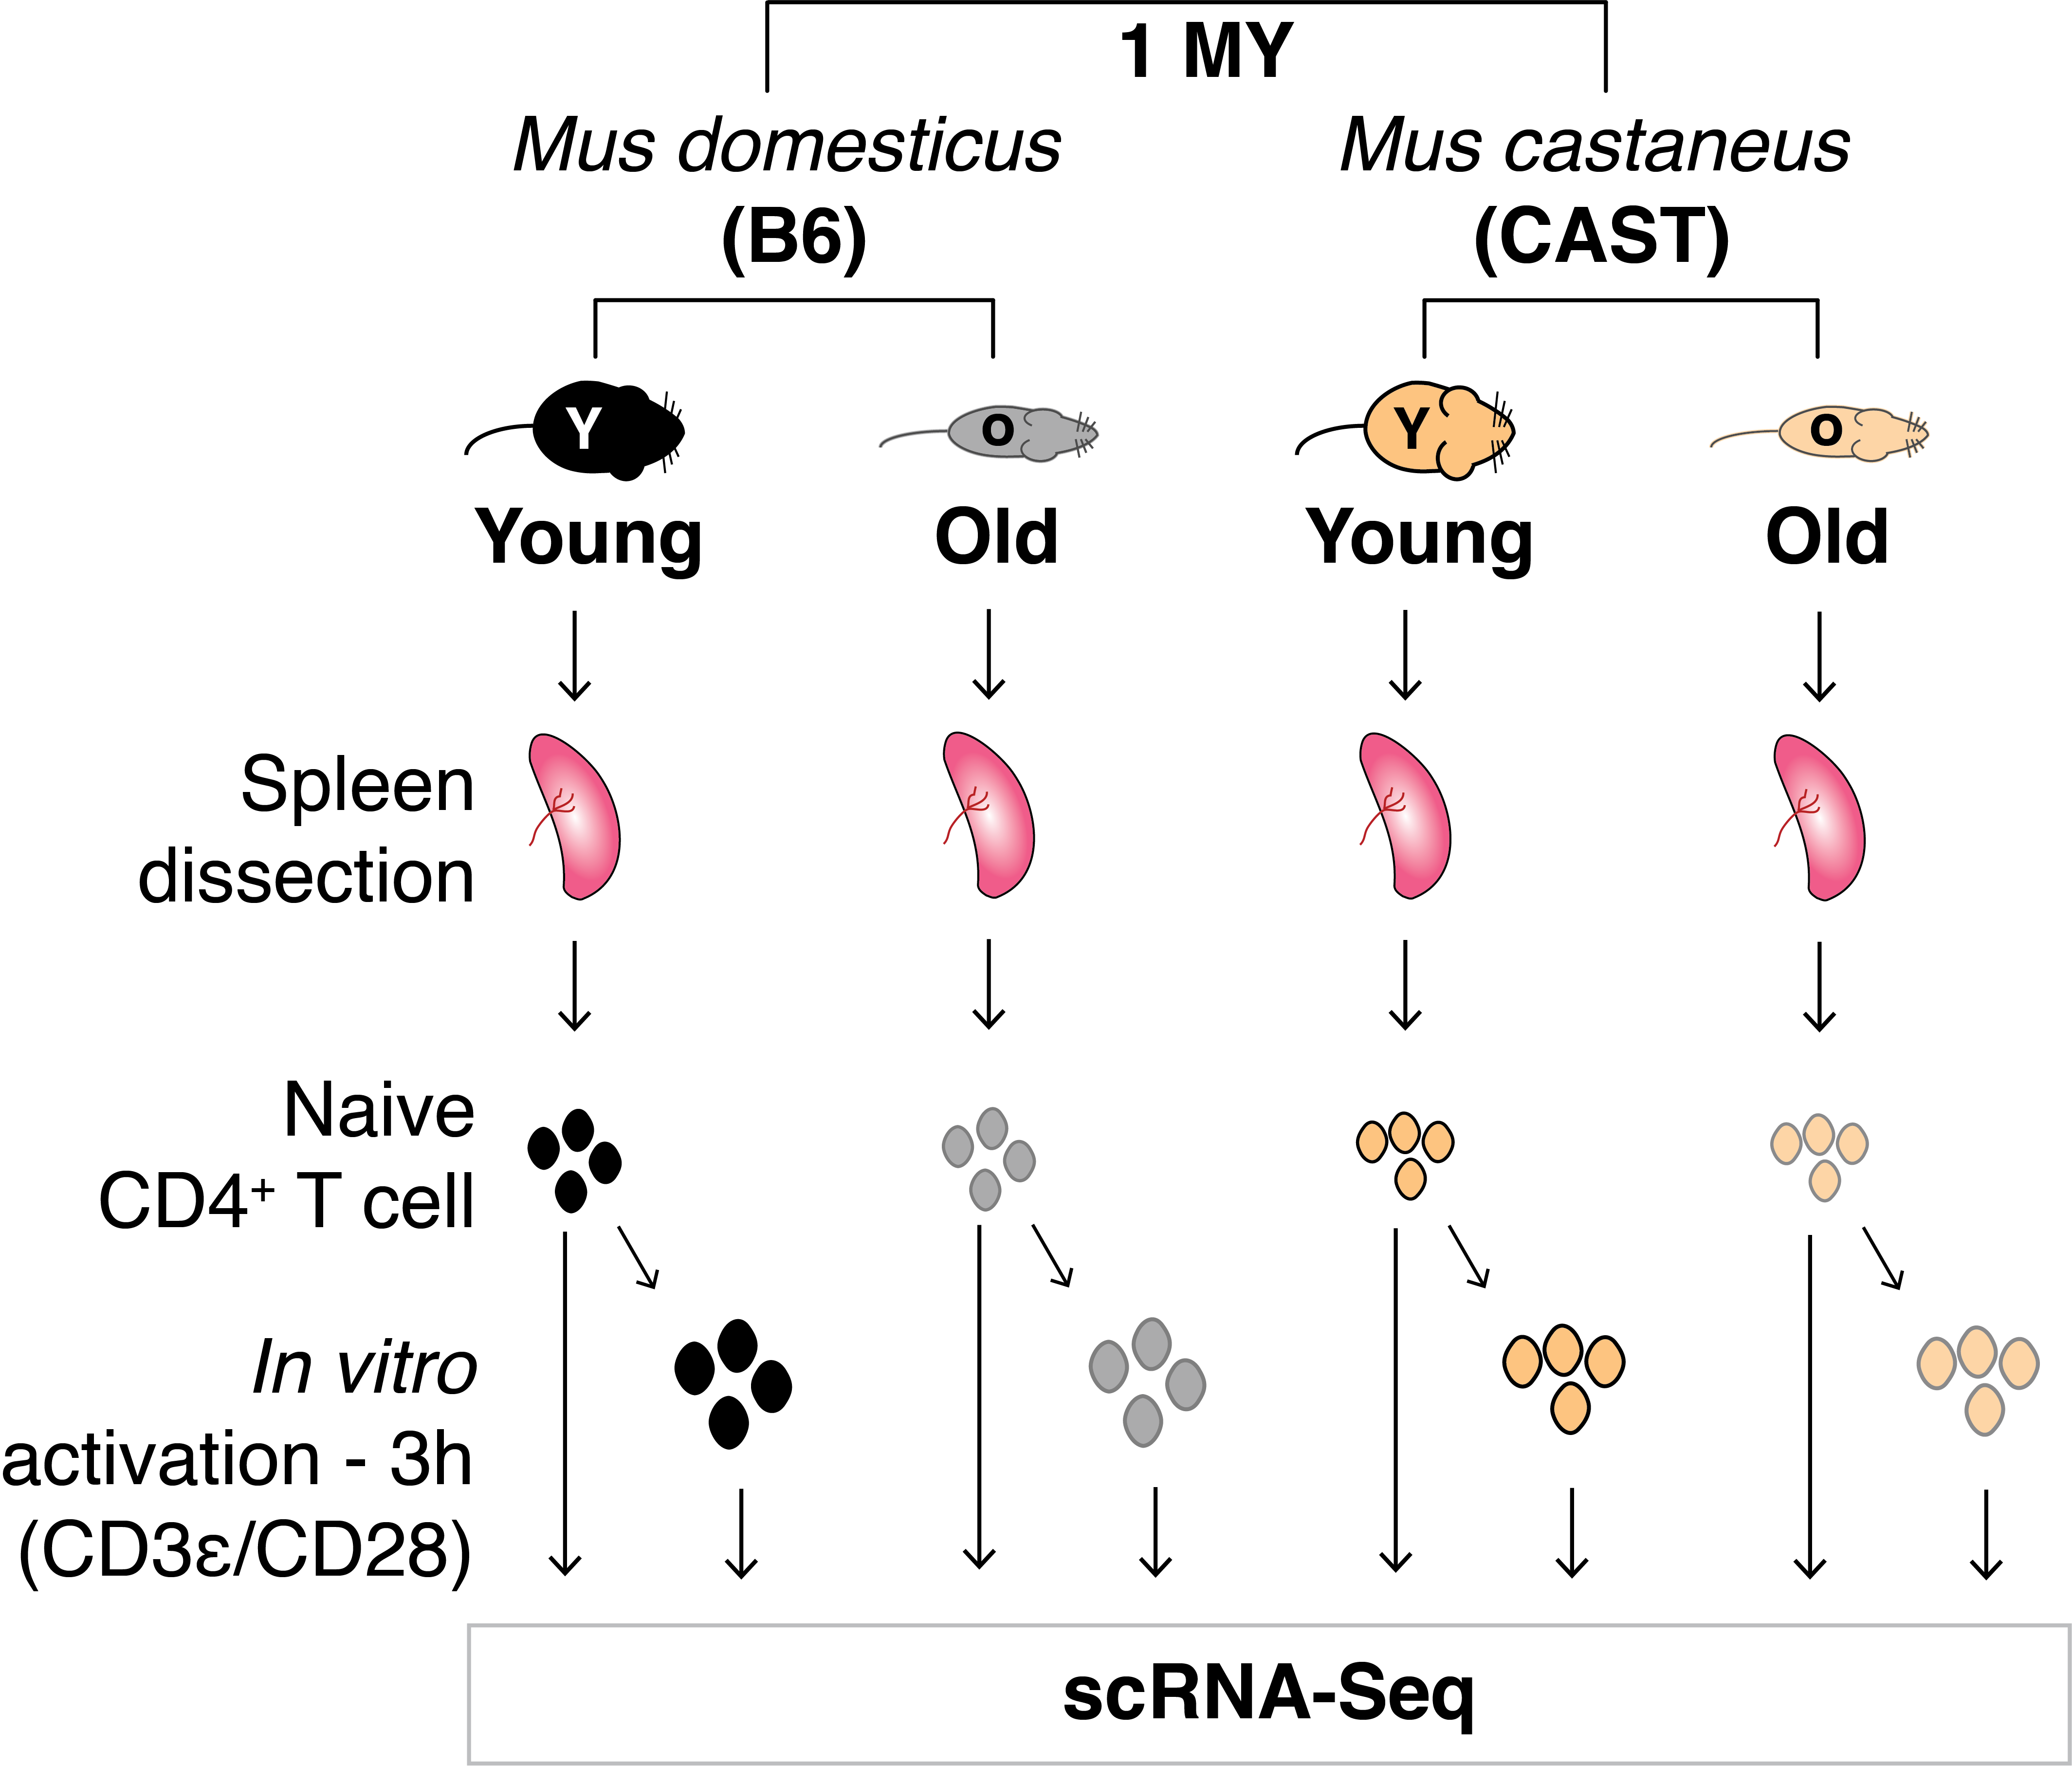
\includegraphics[width=\textwidth]{Fig_1.png}
\caption[Staging of the testicular seminiferous epithelium]{\textbf{Staging of the testicular seminiferous epithelium (full legend on next page).}\\}
\label{fig3:cell_staging}
\end{figure}

\newpage

\captionsetup[figure]{list=no}
\addtocounter{figure}{-1}   
\captionof{figure}{\textbf{Staging of the testicular seminiferous epithelium (continued).}\\
\textbf{(A)} Periodic Acid Schiff (PAS)-stained testis cross-section showing a number of seminiferous tubules at different epithelial stages (displayed as Roman numerals). Within each tubule, the inset circle refers to the corresponding section in (B). Scale bar represents 100 µm; original magnification 200X. \textbf{(B)} Schematic representation of the 12 stages of the seminiferous epithelium in mice. The colour gradient within the circle indicates the differentiation path of germ cells with the layers corresponding to individual cycles of the epithelium. The circle is divided into 12 section, each corresponding to one epithelial stage displaying the characteristic germ cells. Within each section, cells are positioned across the different layers according to their emergence during consecutive cycles, each being 8.6 days apart with more mature cells moving towards the centre.  Cell types are labelled as: A – type A spermatogonia (SG), In – intermediate SG, B – type B SG, Pl – preleptotene spermatocytes (SCs), L – leptotene SCs, Z – zygotene SCs, P – pachytene SCs, D – diplotene SCs, M – metaphase I and II, 1-8 round spermatids, 9-16 elongating spermatids. \textbf{(C)} Higher magnification of two tubules depicted in (A). The PAS-stained cross-sections depict tubules in Stage VII and Stage X, with the different cell layers indicated by coloured lines. Stage VII tubules contain 4 different layers with germ cells from different generations that are approximately 8.6 days apart, whereas Stage X tubules only contain three layers. Each layer contains a certain set of germ cells depending on the epithelial stage. Stage VII contains preleptotene spermatocytes (Pl) in the first layer, pachytene spermatocytes (P) in the second layer, S7 round spermatids (7) in the third layer and S16 elongating spermatids in the fourth innermost layer. Stage X tubules contain leptotene spermatocytes (L) in the first layer, pachytene spermatocytes (P) in the the second layer and only one generation of round-to-elongating spermatids at S10 (10) in the innermost layer. Original magnification 400X.  \\}
\captionsetup[figure]{list=yes}

\todo{Add full experimental methods to appendix}

To fully dissect mouse spermatogenesis, we primarily analysed droplet based single-cell RNA sequencing using the 10X Chromium technology \citep{Zheng2017}. For this, mouse testes were enzymatically dissociated and single-cell suspensions at a concentration of ~300,000 cells/ml was loaded into one channel of the ChromiumTM Single Cell A Chip (10X Genomics), aiming for a recovery of 4000-5000 high-quality cells. Cells were isolated from specifically staged juvenile (between postnatal days 6 and 35) and adult (8-9 weeks) C57BL/6J (B6) mice \textbf{(Table \ref{tab3:QC_scRNAseq})}. To obtain gene-specific transcript counts for droplet based scRNA-Seq, the Cell Ranger \emph{count} function with default settings was used to align and count unique molecular identifiers (UMIs) per sample. This software retains cells with similar UMI distributions \citep{Zheng2017} which we label as "high-quality" transcriptomes. We use this default threshold to obtain high-quality cells with large numbers of UMIs. After merging all samples, we filtered out cells that express less than 1000 genes. Furthermore, we exclude cells with more than 10\% of reads mapping to the mitochondrial genome. \\
Using the Cell Ranger default threshold leads to the exclusion of cells with lower transcriptional complexity. We therefore used the emptyDrops function provided in the \emph{DropletUtils} Bioconductor package \citep{Lun2018} to statistically distinguish empty droplets from genuine cells (controlling the FDR to 1\%). After merging true cells across all samples, we filtered out cells with less than 500 genes expressed. Furthermore, we excluded cells with more than 10\% or mitochondrial genes expressed \textbf{(Table \ref{tab3:QC_scRNAseq})}. The transcriptomes of quality filtered cells were normalized using the scran package \citep{Lun2016pooling}. After quality control and filtering, we retained more than 20,000 high-quality single cells and over 46,000 cells including the once with lower transcriptional complexity \textbf{(Table \ref{tab3:QC_scRNAseq})}. \\
This two-way approach allows us to (i) dissect molecular processes using high-quality cells and capture all testicular cell types, even cells with low transcriptional complexity.\\

Additionally, for juvenile samples, we generated whole-tissue bulk RNA sequencing, as well as mapping chromatin state in purified cell populations using CUT\&{}RUN (Cleavage Under Targets \& Release Using Nuclease) \citep{Skene2018}. With this, we additionally generated 30 bulk RNA-Seq libraries and 8 CUT\&{}RUN libraries.The full experimental set-up can be seen in \textbf{Fig.~\ref{fig3:experimental_design}}.

\begin{figure}[!h]
\centering
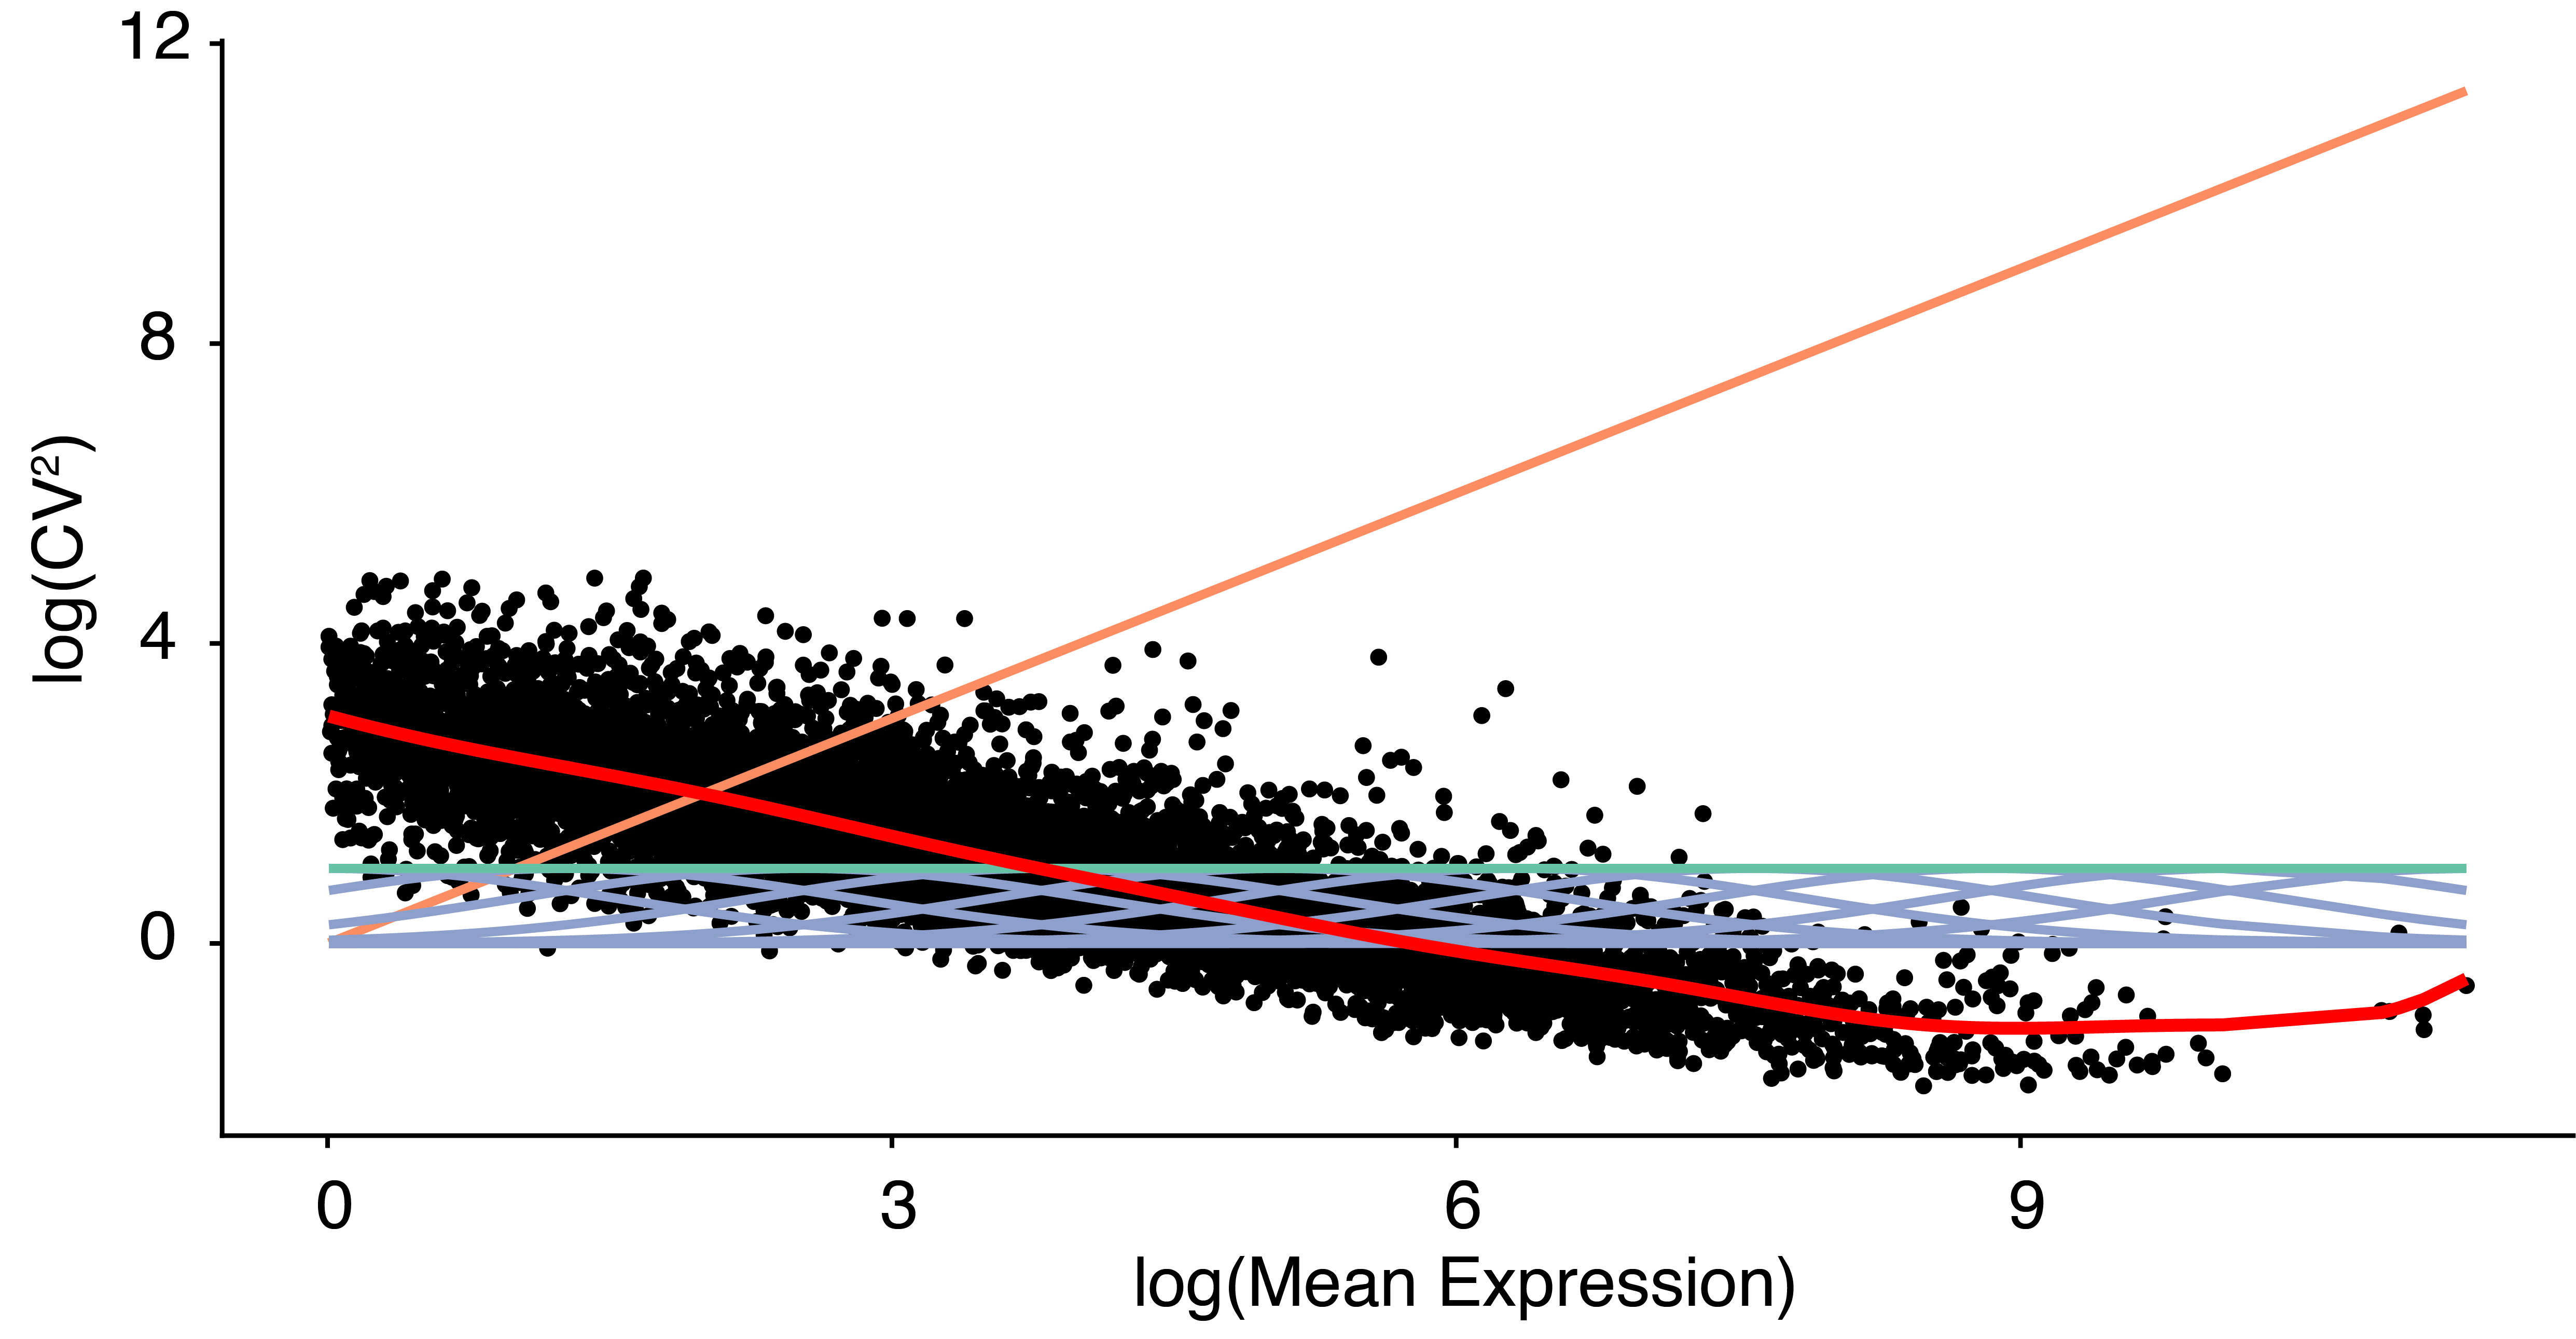
\includegraphics[width=\textwidth]{Fig_2.png}
\caption[Experimental design to dissect mouse spermatogenesis]{\textbf{Experimental design to dissect mouse spermatogenesis.}\\
Overview of the experimental design yielding bulk RNA-Seq, droplet-based scRNA-Seq and chromatin profiling on FACS-purified cells using CUT\&{}RUN from one testis while using the contralateral testis for matched histology.}
\label{fig3:experimental_design}
\end{figure}

To remove batch-specific effects that arise when samples are prepared and sequenced in different experiments \textbf{(Tables \ref{tab3:QC_scRNAseq})}, we used the \emph{mnnCorrect} function implemented in the \emph{scran} package \citep{Haghverdi2018}. We used the top 1000 genes with highest biological variation across all samples as informative genes for batch correction. The \emph{mnnCorrect} function takes transcriptional profiles of cells isolated from adult B6 mice as first input and uses this dataset as reference for cell mapping. This approach maps the juvenile samples onto the adult B6 \textbf{(Fig.~\ref{fig3:cell_types}A)}

\begin{table}[ht	]
\centering
\caption[Quality filtering of scRNAseq data]{\textbf{Quality filtering of scRNAseq data.} \\
Quality metrics of droplet-based scRNA-Seq. Sample: Stage and genotype information for all samples. Library: sample identifier. CellRanger filter: Number of retained cells after default thresholding using the CellRanger counts function.  After quality control: Number of cells obtained after quality control. Assigned Cell Type: Number of cells that fall into annotated clusters (removing outlying cells). EmptyDrops filter: Number of cells retained after using the emptyDrops function controling the FDR to 1\%. EmptyDrops quality control: Number of cells obtained after quality control of the \emph{emptyDrops} filtered cells.}
\label{tab3:QC_scRNAseq}
\begin{tabular}{lllllll}
\toprule
\textbf{Sample} & \textbf{Library} & \textbf{CellRanger} & \textbf{After} & \textbf{Assigned} & \textbf{EmptyDrops} & \textbf{EmptyDrops} \\
& & \textbf{filter} & \textbf{QC} & \textbf{Cell Type} & \textbf{filter} & \textbf{QC} \\
\midrule
B6     & do17815 & 1157              & 1157                  & 1123               & 4467              & 3400                       \\
\midrule
B6     & do17816 & 2198              & 2198                  & 2092               & 6145              & 4603                       \\
\midrule
P10    & do17821 & 3229              & 3213                  & 3212               & 4976              & 4202                       \\
\midrule
P15    & do18195 & 4258              & 4258                  & 4014               & 14050             & 13168                      \\
\midrule
P20    & do17824 & 1775              & 1775                  & 1662               & 9400              & 7491                       \\
\midrule
P25    & do18196 & 4334              & 4334                  & 4130               & 8038              & 6802                       \\
\midrule
P30    & do17825 & 2278              & 2278                  & 2211               & 5393              & 4958                       \\
\midrule
P35    & do17827 & 3160              & 3160                  & 3004               & 49002             & 10683                      \\                 
\bottomrule   
\end{tabular}
\end{table}

To identify cell types across all samples, batch corrected transcriptomes were clustered using a graph-based approach. A shared nearest-neighbour (SNN) graph \citep{Xu2015} was constructed considering 3 shared nearest neighbours using the \emph{buildSNNGraph} function in scran. In the next step, a multi-level modularity optimization algorithm was used to find community structure in the graph \citep{Blondel2008} implemented in \emph{igraph} R package. Cells in small clusters that show unclear identities were excluded from down-stream analysis.\\
We next aimed to annotate clusters based on the expression of marker genes. The adult B6 samples were used to identify marker genes for all germ cell-types present in testes. To this end, we performed differential expression testing across multiple pairwise comparisons. To detect cluster-specific marker genes, the \emph{findMarkers} function implemented in \emph{scran} was used on the log$_2$-transformed normalized counts while providing the cluster labels \textbf{(Fig.~\ref{fig3:cell_types}B)}. \\

On a broad level and by visualizing the expression of detected marker genes, we identified the following cell types: spermatogonia (based on \textit{Dmrt1} expression, \citep{Matson2010}), spermatocytes (\textit{Piwil1}, \citep{Deng2002}), round and elongating spermatids (\textit{Tex21} and \textit{Tnp1}, respectively, \citep{Fujii2002}), as well as the main somatic cell types of the testis, Sertoli (\textit{Cldn11}, \citep{Mazaud-Guittot2010}) and Leydig cells (\textit{Fabp3}, \citep{Oresti2013}) \textbf{(Fig.~\ref{fig3:cell_types}B)}. Using a dimensionality reduction technique for visualization (t-distributed Stochastic Neighbour Embedding; \textbf{Fig.~\ref{fig3:cell_types}C}), the germ cell types from spermatocytes to elongating spermatids formed a continuum, which recapitulated the known developmental trajectory.

\begin{figure}[!h]
\centering
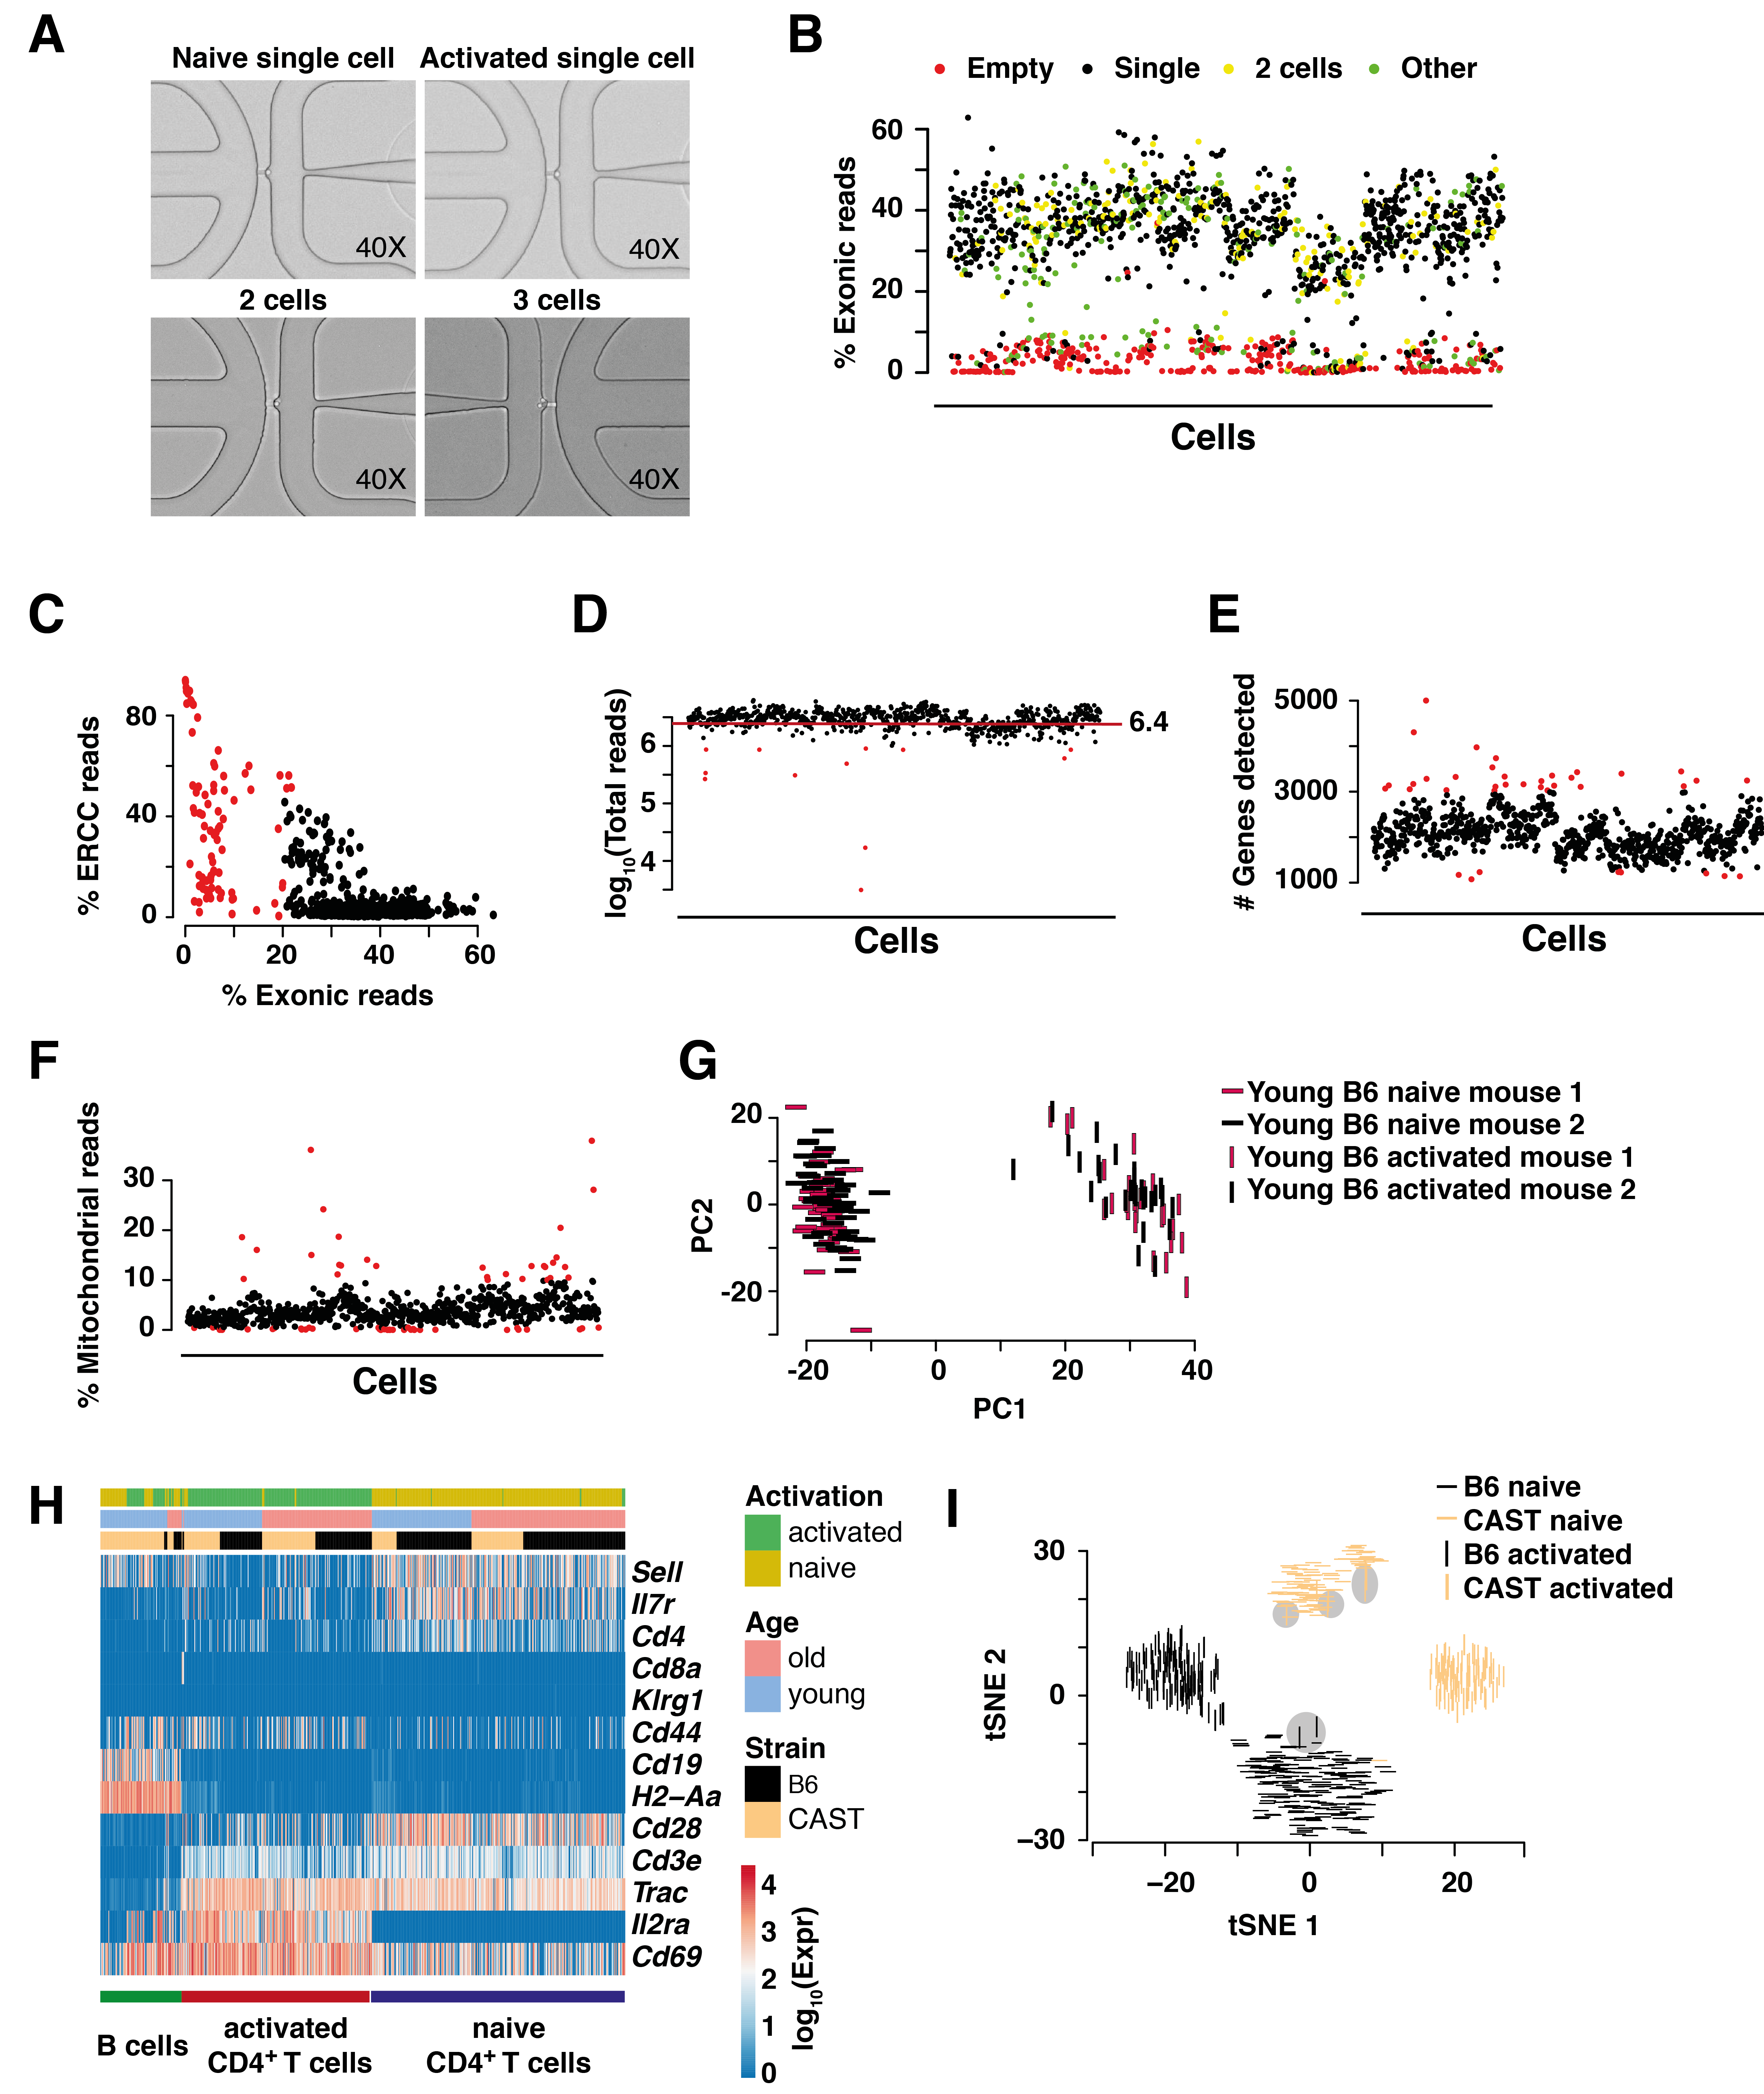
\includegraphics[width=0.8\textwidth]{Fig_3.png}
\caption[Droplet based scRNAseq of mouse spermatogenesis]{\textbf{Single-cell RNA-Seq captures a continuum of germ cell types during adult spermatogenesis.}\\
\textbf{(A)} tSNE representation of juvenile cells that were mapped to cells isolated from adult mice. Grey dots indicate all cells from adult animals that were used as a reference for cell mapping (see Methods). Coloured dots represent cells isolated at each sampled stage during the first wave of spermatogenesis. Clustering has been perfomed across all cells after cell mapping (see Methods). SG: Spermatogonia, M: Meiosis, IL: Imature Leydig, PTM: Peritubular Myoid Cells, EC: Endothelial Cells, tMg: testicular Marcophages. \textbf{(B)} tSNE representation of scRNA-Seq data from adult B6 mice with the colour gradient representing the expression of known marker genes for two somatic cell types and the main germ cell types. The x- and y-axis represent the first and second dimension of tSNE respectively. The colour legend shows log2-transformed, normalized expression counts. \textbf{(E)} Graph-based clustering (see Methods) identifies different sub-stages within major germ cell populations. 
}
\label{fig3:cell_types}
\end{figure}

\section{Developmental staging of mouse spermatogenesis}
\subsection*{Staged developmental mapping of the first wave of spermatogenesis defines germ cell identity}

Historically, sub-staging of the major cell types within the testis was based on changes in nuclear or cellular morphology \citep{Oakberg1956,  Oakberg1956a}. Previous attempts to complement morphology with molecular signatures have been limited to FACS-based and sedimentation assays, where the resolution was unable to differentiate between sub-cell-types \citep{Bastos2005, Gaysinskaya2014, Lam1970, Meistrich1977, Romrell1976, Soumillon2013}. While a mixture of all spermatogenic cell types co-exists in the adult, the first wave of spermatogenesis during juvenile development is more synchronised. Starting around mouse postnatal day P4, spermatogonia begin to differentiate, forming the first generation of spermatocytes as early as P10, round spermatids by P20, and completing the first wave of spermatogenesis with the production of mature spermatozoa between P30 and P35 \textbf{(Fig.~\ref{fig3:1st_wave}A)} \citep{Bellve1977, Janca1986, Nebel1961}.\\
 
We exploited this first spermatogenic wave to generate thousands of high-resolution single-cell transcriptional profiles of morphologically well-defined cell populations. For this, we sampled multiple time points during the first wave to identify the most mature (differentiated) cell types. Based on known sperm developmental transitions, we chose six time points between P10 and P35 from which to generate single-cell RNA-Seq libraries \textbf{(Fig.~\ref{fig3:1st_wave}A)}. For each juvenile experiment, we found that the population of developing germ cells was strongly enriched at the expected developmental stage, as quantified by the percentage of cells in each cell-type cluster \textbf{(Fig.~\ref{fig3:1st_wave}B and C)}. By associating these cell types with the corresponding cell types in the adult trajectory, we unambiguously assigned molecular and histological signatures to cells during adult spermatogenesis.\\

For instance, at P15 the majority of cells are spermatogonia and spermatocytes progressing through the mid-pachytene stage, in accord with the appearance of the sex body \citep{Turner2004}. Interestingly, less mature cell types are also present at this time point (and later time points), supporting recent reports that the first wave of spermatogenesis is less synchronized than previously anticipated \citep{Snyder2010}. At P20, we detect an enrichment for spermatocytes, cells undergoing meiotic cell division, and a small group of early round spermatids. This population structure is in line with matched histology, which shows a large number of tubules in late stages IX-XII and the first occurrence of early round spermatids \citep{Bellve1977}.\\
Spermatids first reach the elongating state between P24 and P26 \citep{Janca1986}. At P25, we observed cells matched to our first ten clusters of spermatids, which we then labelled according to morphologically-defined spermatid substages S1 – S10 \textbf{(Fig.~\ref{fig3:1st_wave}C)}. At P30 and P35, we observed a relatively even distribution of cells across all groups, closely resembling the adult distribution up to S14, indicating that the first wave of spermatogenesis is complete. 

\begin{figure}[!h]
\centering
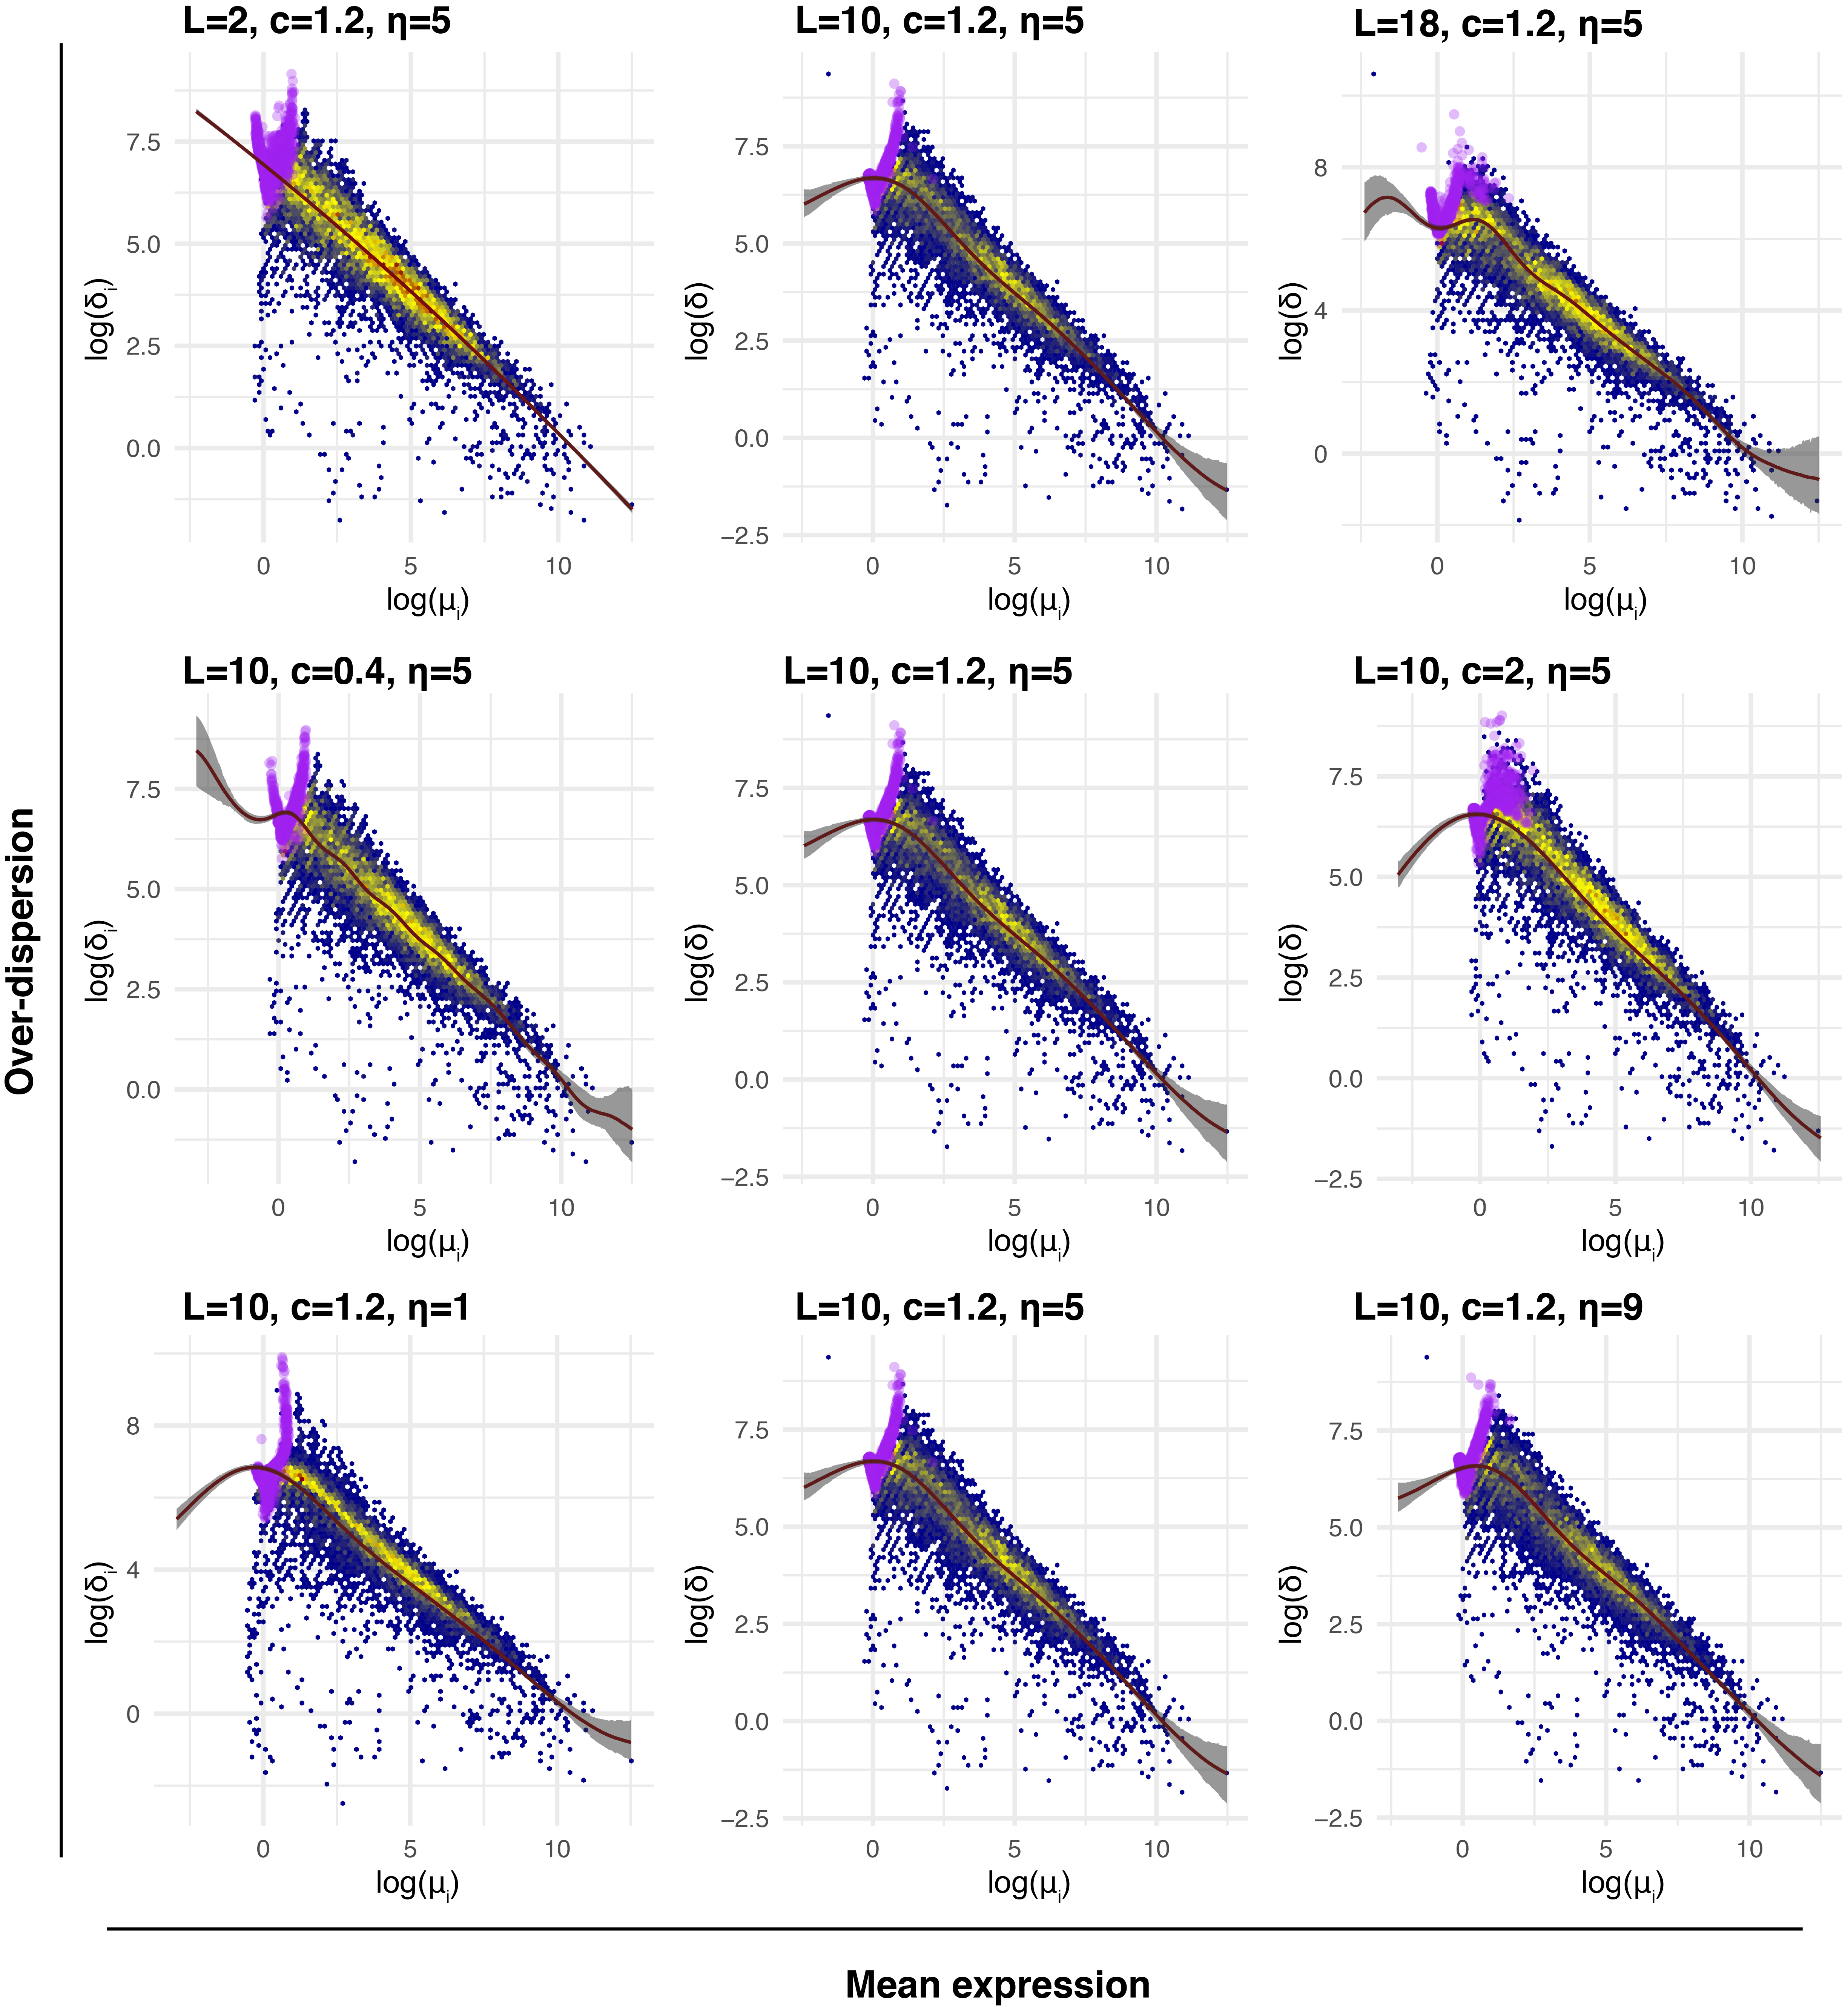
\includegraphics[width=0.85\textwidth]{Fig_4.png}
\caption[Staging of cell types during mouse spermatogenesis]{\textbf{Cell type classification by developmental mapping of time points during the first wave of spermatogenesis (full legend on next page).}}
\label{fig3:1st_wave}
\end{figure}

\newpage

\captionsetup[figure]{list=no}
\addtocounter{figure}{-1}   
\captionof{figure}{\textbf{Cell type classification by developmental mapping of time points during the first wave of spermatogenesis (continued).}\\
\textbf{(A)} Schematic representation of the major germ cell types and their corresponding developmental processes. Spermatogonia differentiate undergoing mitotic cell divisions before forming spermatocytes that divide by meiotic division. Spermatids differentiate throughout spermiogenesis to form mature sperm. The timeline in the lower panel indicates at which point during the first wave of spermatogenesis samples were harvested for the generation of scRNA-Seq (X) or bulk RNA-Seq (B) data. \textbf{(B)} Representative images of seminiferous tubules from PAS-stained tissue cross-sections from animals harvested at different postnatal (P) time points during the first wave of spermatogenesis. The approximate timing of the stage and cycle of the tubule is illustrated below in the form of a circle (see Fig.~\ref{fig3:cell_staging}B). \textbf{(C)} The percentage of cells allocated to each cell cluster for each juvenile and adult sample is represented by the size of squares with the colours corresponding to the clusters depicted in Fig. \ref{fig3:cell_types}C. tSNEs on the right-hand side of each panel (juvenile samples only) illustrate progress through spermatogenesis.  SG – spermatogonia, M – metaphase. \textbf{(D)} Probabilistic mapping of bulk RNA-Seq libraries to the cell clusters identified in the adult scRNA-Seq data using a random forest approach. The colour gradient indicates the probability with which a bulk sample can be assigned to the specific cell cluster.  \\}
\captionsetup[figure]{list=yes}

To further validate the identity of the cell clusters, we used bulk RNA-Seq from testis collected during the first wave of spermatogenesis every two days between P6 and P34 \textbf{(Fig.~\ref{fig3:1st_wave}A)}. We used a regression approach to link the bulk samples to the transcriptomic profiles of single cells. Using the top 50 cluster-specific marker genes for spermatogonia, all spermatocyte groups, all spermatid groups, sertoli and leydig cells, we trained a random forest classifier (implemented in the \emph{randomForest} R package \citep{Liaw2002}) on 2000 cells isolated from adult B6 testes. Model testing was performed on the remaining 1215 cells isolated from adult B6 testes. Prior to training and testing, log$_2$-transformed, normalized counts were scaled by computing the Z score for each gene. Probabilistic prediction was performed using the Z score of log$_2$-transformed, normalized bulk RNA-Seq reads of the input genes. This confirmed that between P6 – P14 spermatogonia and somatic cells show the highest contribution to the transcriptomic profile \textbf{(Fig.~\ref{fig3:1st_wave}D)}. Between P16 and P20 we observed the emergence of spermatocyte-specific gene expression signatures, after which spermatids become the transcriptionally dominant cell type. By P26, spermatids reach the elongating state where transcription is uniformly shut-down due to the beginning of the histone-to-protamine transition \citep{Steger1999}; following this, changes in RNA content are mostly due to degradation. Bulk transcriptional profiles can therefore only be classified up to S10, because transcription is largely inactive thereafter.\\

In sum, by combining transcriptional and histological analyses at specific stages during the first wave of spermatogenesis, we assigned transcriptional profiles to specific, morphologically defined germ cell types.

\section{Under-represented cell types in spermatogenesis}
\subsection*{Identification of under-represented and transcriptionally silent cell types in adolescent testes}

In addition to assigning the dominant cell types in germ cell development, we further exploited the juvenile samples to analyse the highly enriched cell types that are rare in adult testes, including somatic support cells, spermatogonia and the earliest spermatocytes.  Through the first wave of spermatogenesis, the ratio between germ cells and somatic cells increases; therefore, to study heterogeneity within the somatic cell population, we focused on the P10 stage, where somatic cells are relatively more frequent. As expected, we readily identified substantial numbers of Sertoli and Leydig cells, which are the main somatic cell types in adult \citep{Griswold1998, Haider2004}.  In addition, we newly identified a large population of immature Leydig cells, based on \textit{Dlk1} expression \citep{Lottrup2014}. Furthermore, we detected the cells that form the basal lamina such as peritubular myoid cells (PTM, \textit{Acta2}, \citep{Cool2008}), vascular endothelial cells (\textit{Tm4sf1}, \citep{Shih2009}), and testicular macrophages (\textit{Cd14}, \citep{Kitchens2000}) \textbf{(Fig.~\ref{fig3:somatic_cells}A and B)}. By performing differential expression analysis, we identified novel markers for these cell populations that are relatively under-represented in adult testes.\\

\begin{figure}[!h]
\centering
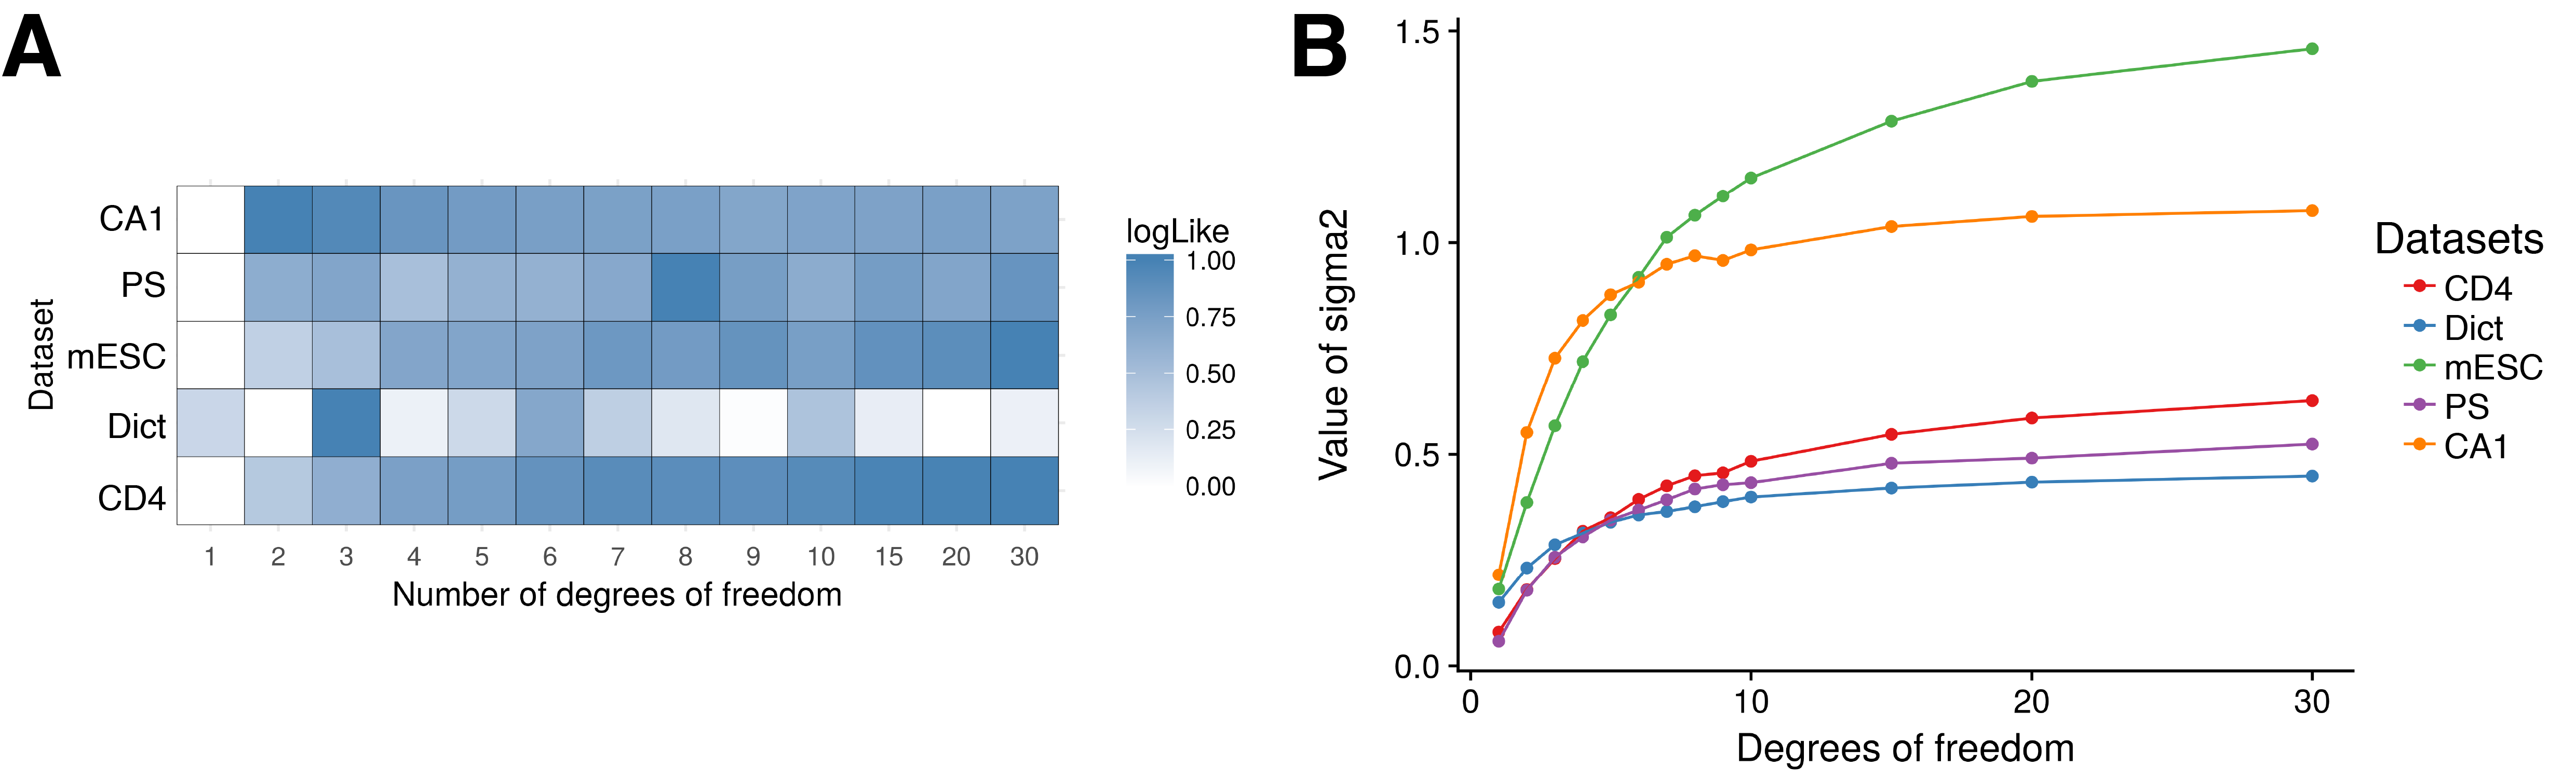
\includegraphics[width=\textwidth]{Fig_5.png}
\caption[Enrichment of under-represented somatic cell types in juvenile samples]{\textbf{Enrichment of underrepresented somatic cell types in juvenile samples.} \\
\textbf{(A)} tSNE representation of cells isolated from P10 animals that were mapped to cells from adult mice. Cell types were identified by unbiased, graph-based clustering and annotated after marker gene extraction. SG: Spermatogonia, SC: Spermatocytes, IL: Immature Leydig, PTM: Peritubular Myoid Cells, EC: Endothelial Cells, tMg: testicular Macrophages. \textbf{(B)} Heatmap representation of cell type-specifc marker genes. Bolded genes indicate previously described markers for the following cell types: Sertoli cells (\textit{Cst12}), early spermatocytes (\textit{Sycp1}), spermatogonia (\textit{Dmrt1}), immature leydig cells (\textit{Dlk1}), endothelial cells (\textit{Acta2}), peritubular myoid cells (\textit{Tm4sf1}), Leydig cells (Insl3), testicular macrophages (\textit{Cd14}). \textbf{(C)} PCA of spermatogonia (SG) and early spermatocytes (SC 1) from P10 and P15 animals. 
}
\label{fig3:somatic_cells}
\end{figure}

In the mouse, this differentiation process initiates with the division of a spermatogonial stem cell (SSC or A$_{\text{single}}$) to form first a pair, and then a connected chain, of undifferentiated spermatogonia (A$_{\text{paired}}$ and A$_{\text{aligned}}$) \citep{Oakberg1971, DeRooij1973}. These cells have competency to undergo spermatogonial differentiation, which involves six transit-amplifying mitotic divisions generating A$_{1-4}$, Intermediate, and B spermatogonia, which then give rise to pre-leptotene spermatocytes (pL) \citep{DeRooij2000}

Identifying spermatogonial sub-populations in adult testes is greatly complicated by their rarity relative to other germ cell types \citep{Lukassen2018}. However, during early juvenile development spermatogonia are relatively enriched, which we exploited to further characterize their heterogeneity \textbf{(Fig. \ref{fig3:spermatogonia}A)}. By combining cells from P10 and P15, we obtained 1,186 transcriptional profiles that capture sub-populations during spermatogonial differentiation \textbf{(Fig. \ref{fig3:spermatogonia}B)}. To analyse transcriptomes of P10 and P15 samples, we performed batch correction between these samples as described above. We detected two clusters corresponding to undifferentiated spermatogonia (A$_\textnormal{undiff}$) based on their expression of \textit{Nanos3} and \textit{Zbtb16} \textbf{(Fig. \ref{fig3:spermatogonia}B and C)} \citep{Buaas2004, Lolicato2008}). These cells comprise A$_\textnormal{s}$, A$_\textnormal{paired}$, and A$_\textnormal{aligned}$ spermatogonia that decrease in stemness as they divide and gain competency to differentiate \citep{Suzuki2012}. Additionally, these cells express a number of marker genes also detected in undifferentiated human spermatogonial stem cells, such as \textit{Gfra1}, \textit{Bcl6} and \textit{Id4} \citep{Guo2017}. Based on the expression of \textit{Stra8} (Stimulated by retinoic acid 8), we can map the point at which spermatogonial differentiation is induced (A$_\textnormal{aligned}$-to-A$_\textnormal{1}$ transition), thus marking the beginning of differentiating spermatogonia (A$_\textnormal{diff}$) \citep{Endo2015}. A$_\textnormal{diff}$ are marked by the expression of \textit{Sohlh1} \citep{Ballow2006} and are highly proliferative, generating A$_\textnormal{1-4}$, Intermediate and B spermatogonia. Late differentiating spermatocytes express \textit{Dmrtb1} (also referred to as \textit{Dmrt6}), which mediates the mitosis-to-meiosis transition and quickly disappears in preleptotene spermatocytes. This latter population shows a second increase in Stra8 expression levels, which is necessary for initiation of meiosis \textbf{(Fig. \ref{fig3:spermatogonia}B and C)} \citep{Anderson2008, Endo2015, Zhang2014}. 

\newpage

\begin{figure}[!h]
\centering
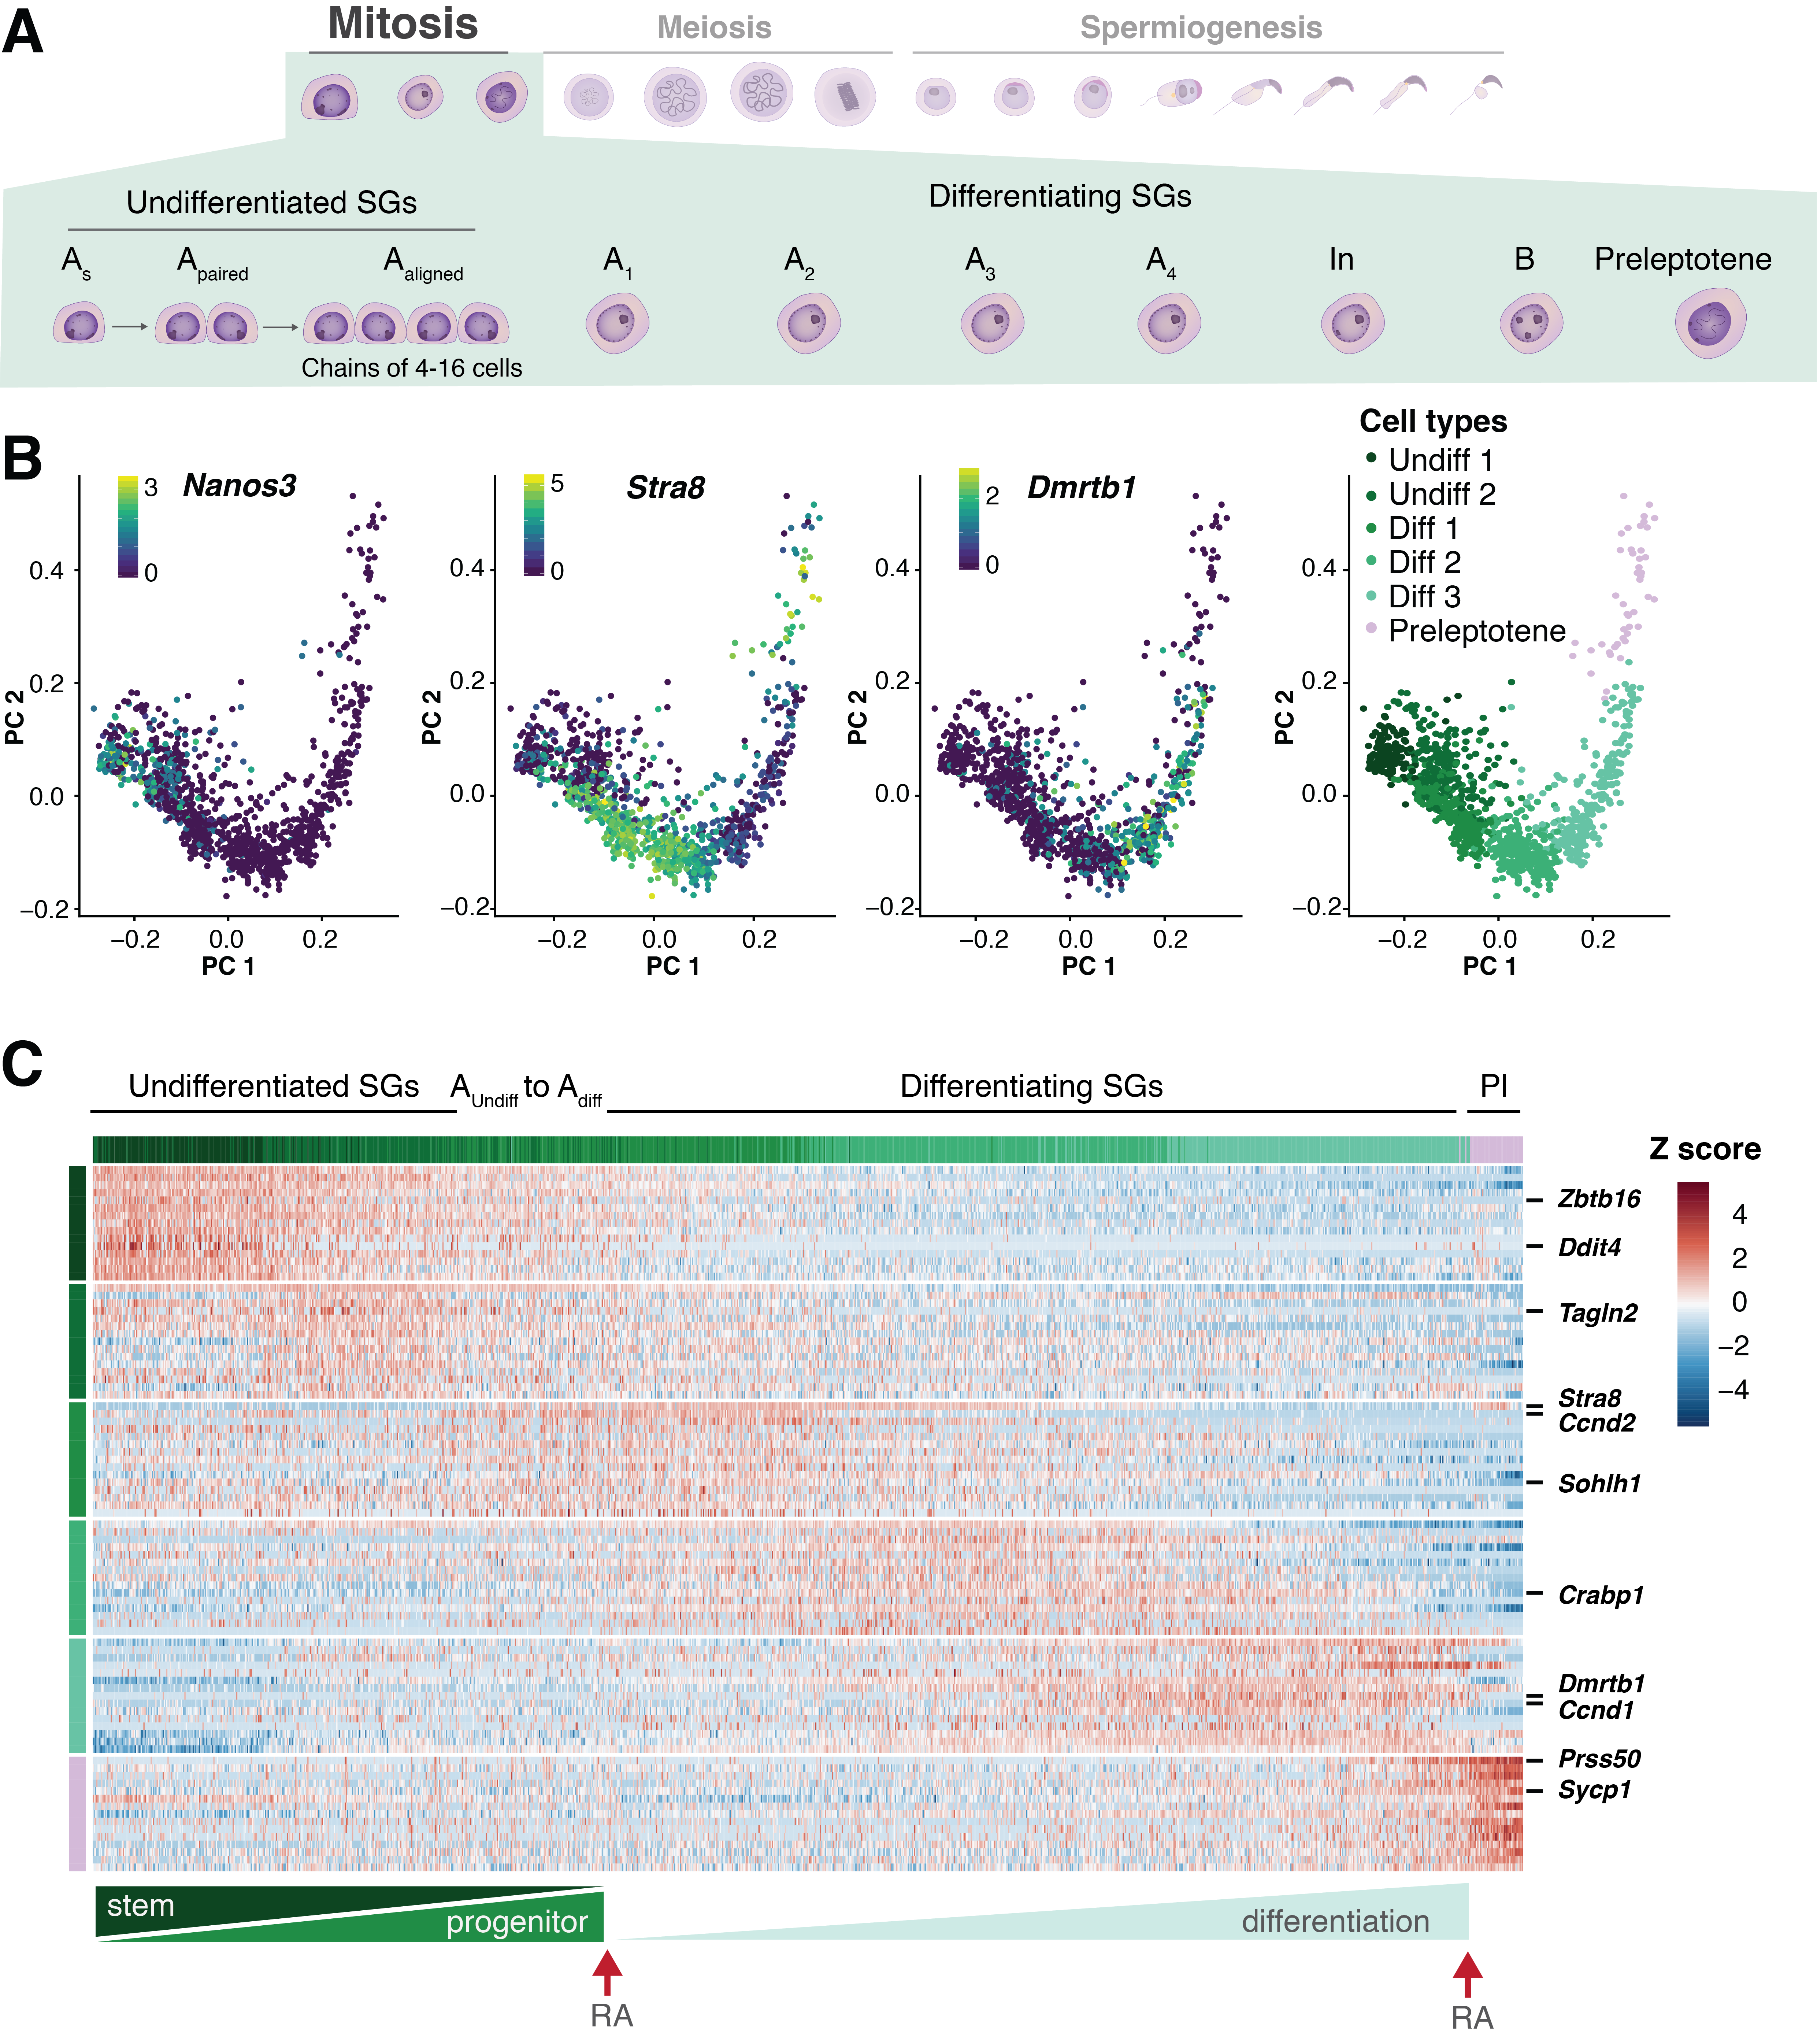
\includegraphics[width=0.85\textwidth]{Fig_6.png}
\caption[Cellular heterogeneity during spermatogonial differentiation]{\textbf{Cellular heterogeneity during spermatogonial differentiation.} \\
\textbf{(A)} Schematic representation of spermatogonial differentiation including sub-stages of undifferentiated (A$_\textnormal{s}$, A$_\textnormal{paired}$, A$_\textnormal{aligned}$) and differentiating spermatogonia (A$_\textnormal{1}$, A$_\textnormal{2}$, A$_\textnormal{3}$, A$_\textnormal{4}$, In, B) (SGs) as well as Preleptotene (Pl). \textbf{(B)} Sub-structure detection in spermatogonia isolated from P10 and P15 animals. PCA was computed on transcriptomes after batch correction between P10 and P15 samples. The first three panels represent expression of known marker genes for undifferentiated (Undiff, \textit{Nanos3}) and differentiating (Diff, \textit{Stra8} and \textit{Dmrtb1}) spermatogonia. The colour scale shows log$_2$-transformed, normalized counts. The last panel overlays cluster identity by sub-clustering batch-corrected transcriptomes of spermatogonia. \textbf{(C)} Scaled, normalized expression counts of the top 15 marker genes per cell cluster. Column and row labels represent the cell clusters identified in the last panel of (B). The lower bar indicates the gradual differentiation from undifferentiated spermatogonia to preleptotene cells driven by two retinoic acid (RA) signals. }
\label{fig3:spermatogonia}
\end{figure}

The transition between differentiating spermatogonia and spermatocytes is a gradual process that occurs in stage VIII tubules when B spermatogonia divide and form preleptotene spermatocytes \citep{Anderson2008, Baltus2006}. We were therefore surprised not to observe a continuous differentiation trajectory bridging spermatogonia to spermatocytes \textbf{(Fig. \ref{fig3:somatic_cells}C)}. One possible explanation is that leptotene and zygotene spermatocytes have decreased transcriptional activity \citep{Kierszenbaum1974, Monesi1965}, and are thus likely to be classified as empty droplets by the 10X CellRanger pipeline. 
To capture these transcriptionally quiescent cells, we applied a newly developed computational method that distinguishes between droplets capturing genuine cells containing small amounts of mRNA versus empty droplets containing only ambient mRNA \citep{Lun2018}. Applying this approach increased the number of early spermatocytes in all samples and, in particular, identified a population of cells connecting spermatogonia and spermatocytes at the predicted position in the cell trajectory \textbf{(Fig.~\ref{fig3:emptyDrops}A-C)}. As expected for leptotene and zygotene spermatocytes, these cells show high mRNA levels for genes involved in synaptonemal complex formation, chromosome synapsis and DNA double-strand break (DSB) formation such as \textit{Sycp1}, \textit{H2afx} and \textit{Hormad1} \textbf{(Fig.~\ref{fig3:emptyDrops}D)} \citep{Daniel2011, Mahadevaiah2001, Vries2005}.\\
In addition to early spermatocytes, droplets with lower transcriptional complexity also captured late condensing spermatids; as mentioned above, these late stages of spermiogenesis are characterized by continuous degradation of RNA after transcriptional shutdown at the round-to-elongating transition \citep{Steger1999} \textbf{(Fig.~\ref{fig3:emptyDrops}E)}.\\
 
By profiling carefully chosen developmental time points and applying new methods to incorporate single cells with lower transcriptional complexity, our results elucidate a more complete view of testicular cell type composition that includes previously under-represented cell types.

\newpage

\begin{figure}[!h]
\centering
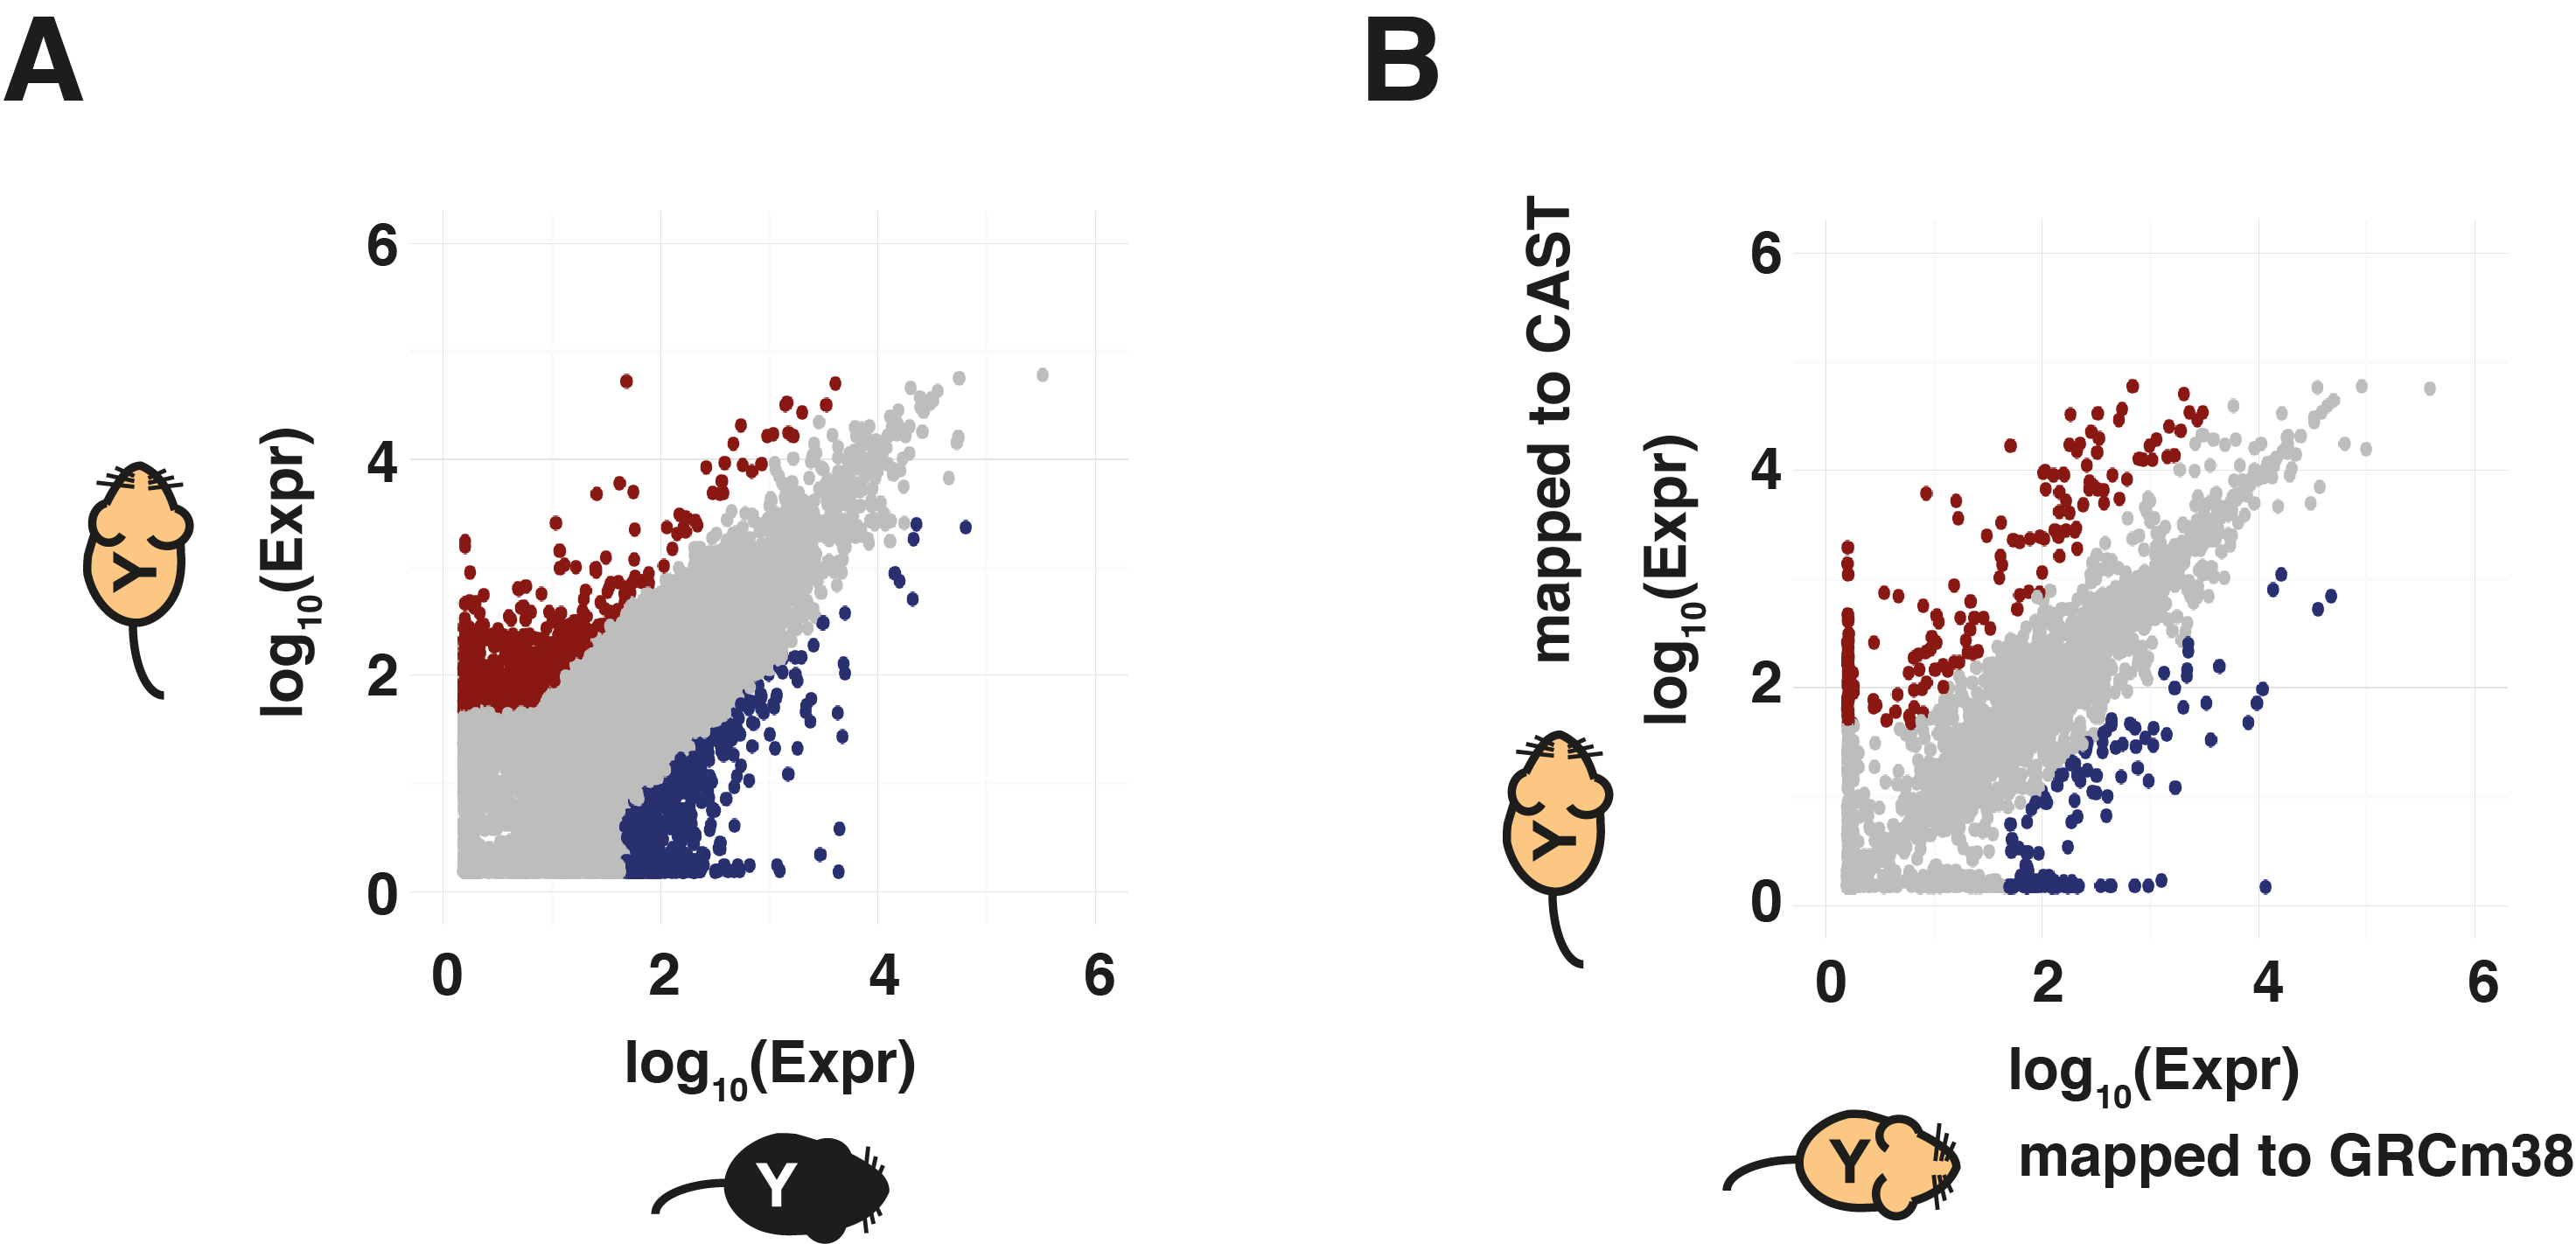
\includegraphics[width=0.8\textwidth]{Fig_7.png}
\caption[Transcriptionally silent cell types in spermatogenesis.]{\textbf{Detection of transcriptionally silent cell types in scRNA-Seq data.} \\
\textbf{(A)} tSNE representation of cells selected by the emptyDrops filtering strategy. Coloured dots represent annotated cell types detected using the default CellRanger filtering pipeline while black dots represent cells detected by the emptyDrops filtering. SG: Spermatogonia, SC: Spermatocytes, IL: Immature Leydig, PTM: Peritubular Myoid Cells, EC: Endothelial Cells, tMg: testicular Macrophages. \textbf{(B)} tSNE representation of emptyDrops filtered cells from the P15 sample. Cell colouring corresponds to clustering performed on this sample. Undiff SG: undifferentiated spermatogonia, Diff SG: differentiating spermatogonia. \textbf{(C)} PCA representation of spermatogonia and spermatocytes detected in the P15 sample after emptyDrops filtering. Labelling corresponds to the clusters shown in (B). \textbf{(D)} Leptotene and zygotene spermatocyte marker gene expression. The colour scale represents log$_2$-transformed, normalized counts. \textbf{(E)} Visualization of the number of genes expressed (> 0 counts) per cell.
}
\label{fig3:emptyDrops}
\end{figure}

\newpage


\section{Characterization of male meiosis}

In contrast to mitosis, meiosis includes programmed DNA double strand break (DSB) formation, homologous recombination, and chromosome synapsis \citep{Marston2004}

The mitotic expansion of spermatogonia produces large numbers of spermatocytes, which then undergo male meiosis where two consecutive cell divisions give rise to four haploid spermatids. In contrast to mitotic cell divisions, prophase of meiosis I is extremely prolonged, lasting up to 10 days in male mice \citep{Soh2017}. This process has been histologically described, but a full transcriptional characterization of spermatocytes undergoing meiosis is lacking. \\

To address this, we ordered spermatocytes along their differentiation trajectory. For this, we fitted a principal curve \citep{Hastie1989} to the first 3 principal components (computed on the top 1000 highly variable genes) using the \emph{principal.curve} function implemented in the \emph{princurve} R package. This approach allows us to order cells along the principal curve. The directionality of the curve was inferred using prior information based on the cluster annotation. Here, the differentiation trajectory starts at the first group of spermatocytes and ends at the meiotic cell divisions. \\
We first identified a strong increase in the number of genes expressed as spermatocytes progress through prophase, with the highest number being expressed immediately before the cells divide \textbf{(Fig.~\ref{fig3:meiosis}A)}. Using this as a proxy for active transcription, we identified diplotene spermatocytes, which are the latest cell type in prophase I in which RNA synthesis is occurring \citep{Monesi1965}. To profile increasing or decreasing transcription throughout meiotic prophase, we correlated each gene’s normalised expression level to the number of genes expressed. For this, we used the \emph{correlatedPairs} function implemented in \emph{scran} \citep{Lun2016}. We first constructed an empirical null distribution using the \emph{correlateNull} function implemented in scran. Next, we tested the observed Spearman’s $\rho$ for each gene against this null distribution.  We consider genes with $\rho$ < -0.3 and a Benjamini-Hochberg corrected empirical p-value < 0.1 as negatively correlated and genes with $\rho$ > 0.3 and a Benjamini-Hochberg corrected empirical p-value < 0.1 as positively correlated. As expected, previously known marker genes for early meiotic processes such as \textit{Hormad1} and \textit{Sycp3} decreased in expression during Prophase I, whereas \textit{Pou5f2} and \textit{Tcte2}, a male-meiosis specific gene \citep{Braidotti1997} increased in expression \textbf{(Fig.~\ref{fig3:meiosis}B)}. Supporting our identification of diplotene spermatocytes, \textit{Pou5f2} has previously been shown to be specifically expressed during a 36- to 48-hour period preceding the meiotic cell division \citep{Andersen1993}. \\

\newpage

\begin{figure}[!h]
\centering
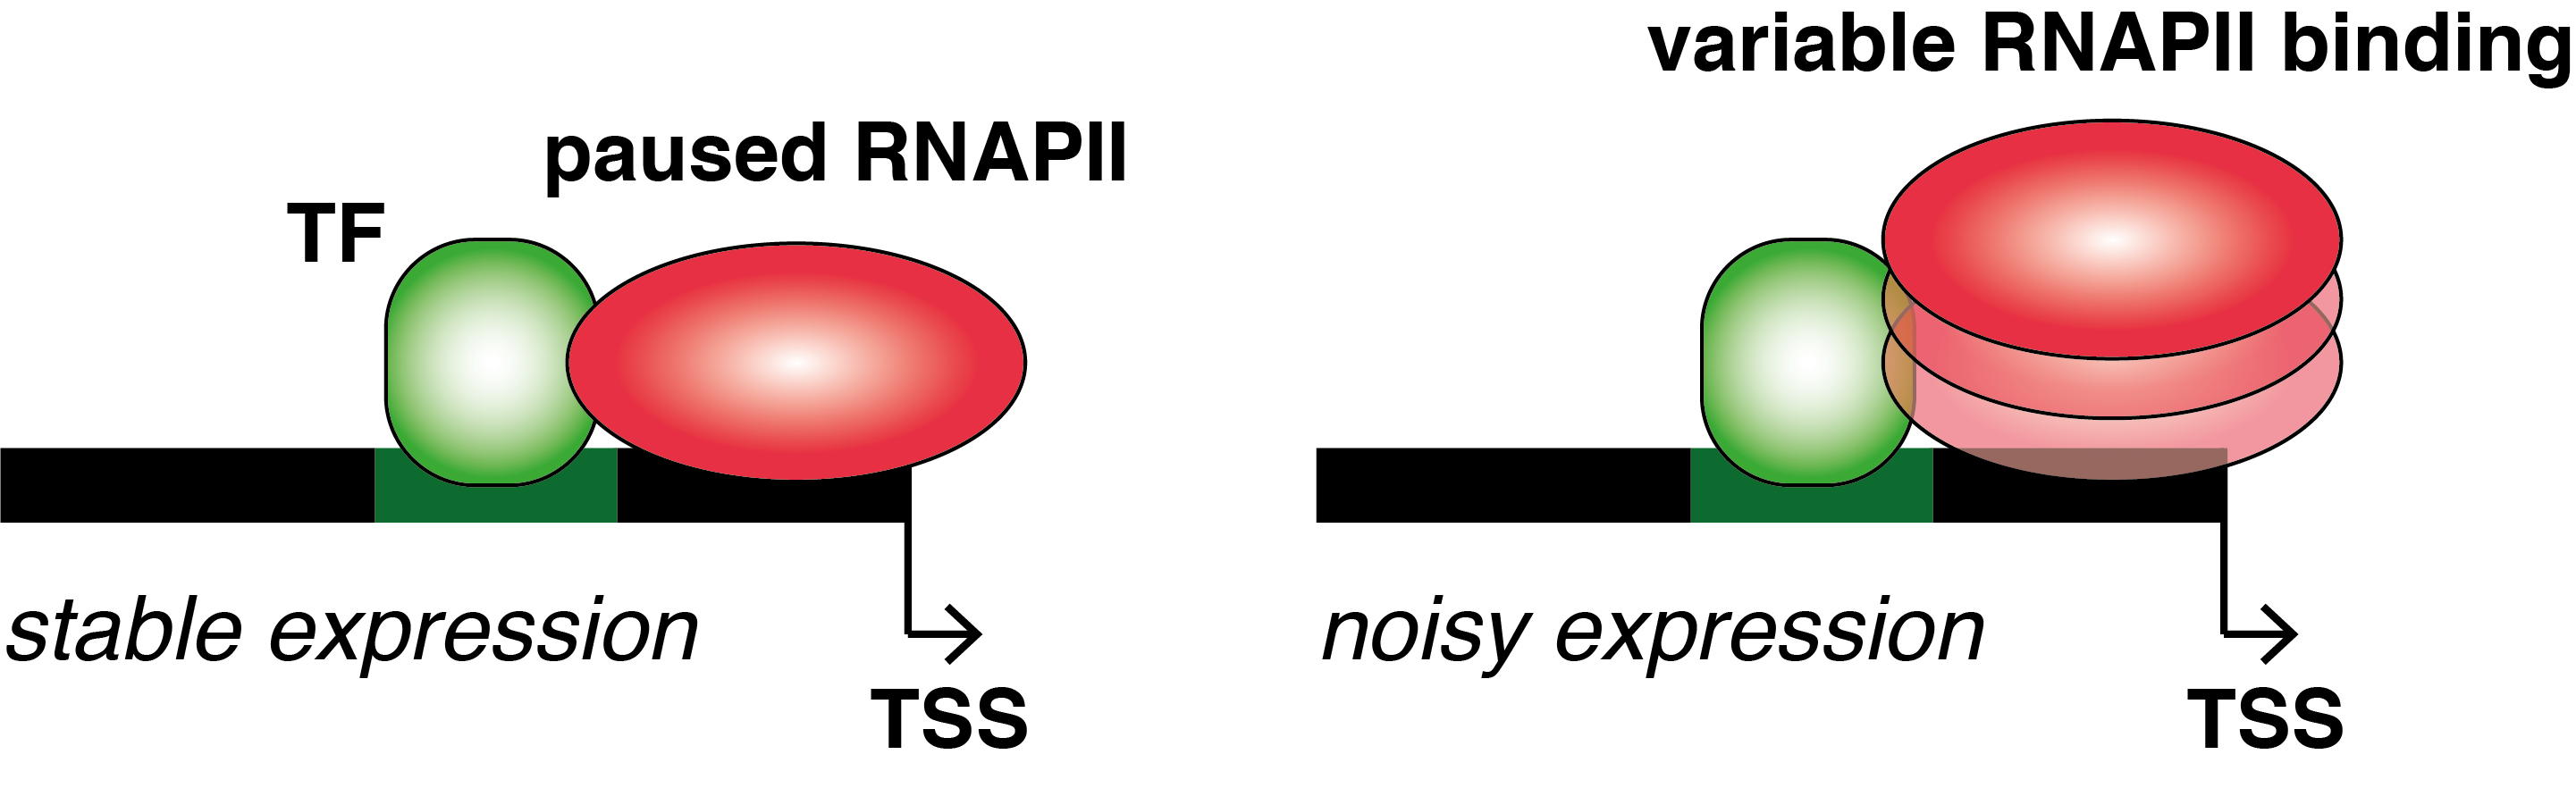
\includegraphics[width=0.9\textwidth]{Fig_8.png}
\caption[Gene expression dynamics during male meiosis]{\textbf{Gene expression dynamics during male meiosis.} \\
\textbf{(A)} Number of genes expressed per spermatocyte. Cells are ordered by their developmental progression during meiotic prophase until metaphase. \textbf{(B)} Expression of genes that are negatively or positively correlated with the number of genes expressed during meiotic prophase (negatively correlated: $\rho$ < -0.3, Benjamini-Hochberg corrected empirical p-value < 0.1; positively correlated: $\rho$ > 0.3, Benjamini-Hochberg corrected empirical p-value < 0.1). Per category, two genes are visualized. The colour gradient represents log$_2$-transformed, normalized counts. \textbf{(C)} Heatmap visualizing the scaled expression of the top 15 marker genes per cell type. Row and column labels correspond to the different populations of spermatocytes (SC). M: Metaphase. Genes are labelled based on their fertility phenotype: pink – infertile or sub-fertile in females, light blue - infertile or sub-fertile in males, dark green - infertile or sub-fertile in both males and females. The sterility phenotype was annotated using www.mousephenotype.org.}
\label{fig3:meiosis}
\end{figure}

Despite the overall increase in transcription, we observed distinct temporal expression patterns when visualizing specific marker genes for individual spermatocyte populations. Even within pachytene spermatocytes at different stages in their developmental progression, there exists substantial heterogeneity \textbf{(Fig.~\ref{fig3:meiosis}C)}. As expected, early spermatocyte markers (SC 1 and SC 2) were enriched for genes with known functions in male or female fertility, reflecting a history of intensive investigation \citep{Deng2002, Spruck2003, Vries2005}. In contrast, our datasets reveal genes present in previously-unknown transcriptional programs that functionally orchestrate the later stages of spermatocyte development.

\section{Transcriptional dynamics during spermiogenesis}
\label{sec3:spermiogenesis}

A key event during spermiogenesis is chromatin condensation, which is required to package the haploid genome into the confined space of the sperm nucleus. Our data allowed us to dissect at high-resolution the gradual chromatin remodelling during spermatid differentiation, involving the replacement of canonical histones by histone variants followed by transition proteins and eventually protamines \citep{Balhorn2007, Kennani2017}. \\

We first explored how expression of histone variants changed throughout early spermatid maturation \textbf{(Fig.~\ref{fig3:spermiogenesis}A)}. Multiple variants of H3 and H2A are expressed in spermatocytes \citep{Greaves2006, Mahadevaiah2001, Tang2015}, and our data showed that many of these histones are highly expressed in early round spermatids. For instance, Histone H3.3 is a histone variant consisting of two genomic copies (\textit{H3f3a} and \textit{H3f3b}). Across spermatogenesis, we observed distinct expression patterns for the two genes, with \textit{H3f3a} being consistently high until the transcriptional shut-down. In contrast, \textit{H3f3b} showed a much more dynamic expression profile, starting high in spermatocytes, dropping throughout meiotic prophase, followed by upregulation in round spermatids \textbf{(Fig.~\ref{fig3:spermiogenesis}B)}. Although both genes have been implicated in male fertility, the phenotypes associated with perturbations of the more dynamically regulated paralog \textit{H3f3b} are much more severe \citep{Tang2015, Yuen2014}.\\

We detected increased expression for particular canonical histones, of which \textit{Hist1h2bp} and \textit{Hist1h4a} showed a distinct up-regulation during early and mid-spermiogenesis \textbf{(Fig.~\ref{fig3:spermiogenesis}C)}. Canonical histones are typically transcribed in a replication-dependent manner during S phase \citep{Marzluff2002}, thus the atypical expression during spermiogenesis could suggest important roles as replacement histones during chromatin remodelling.

\newpage

\begin{figure}[!h]
\centering
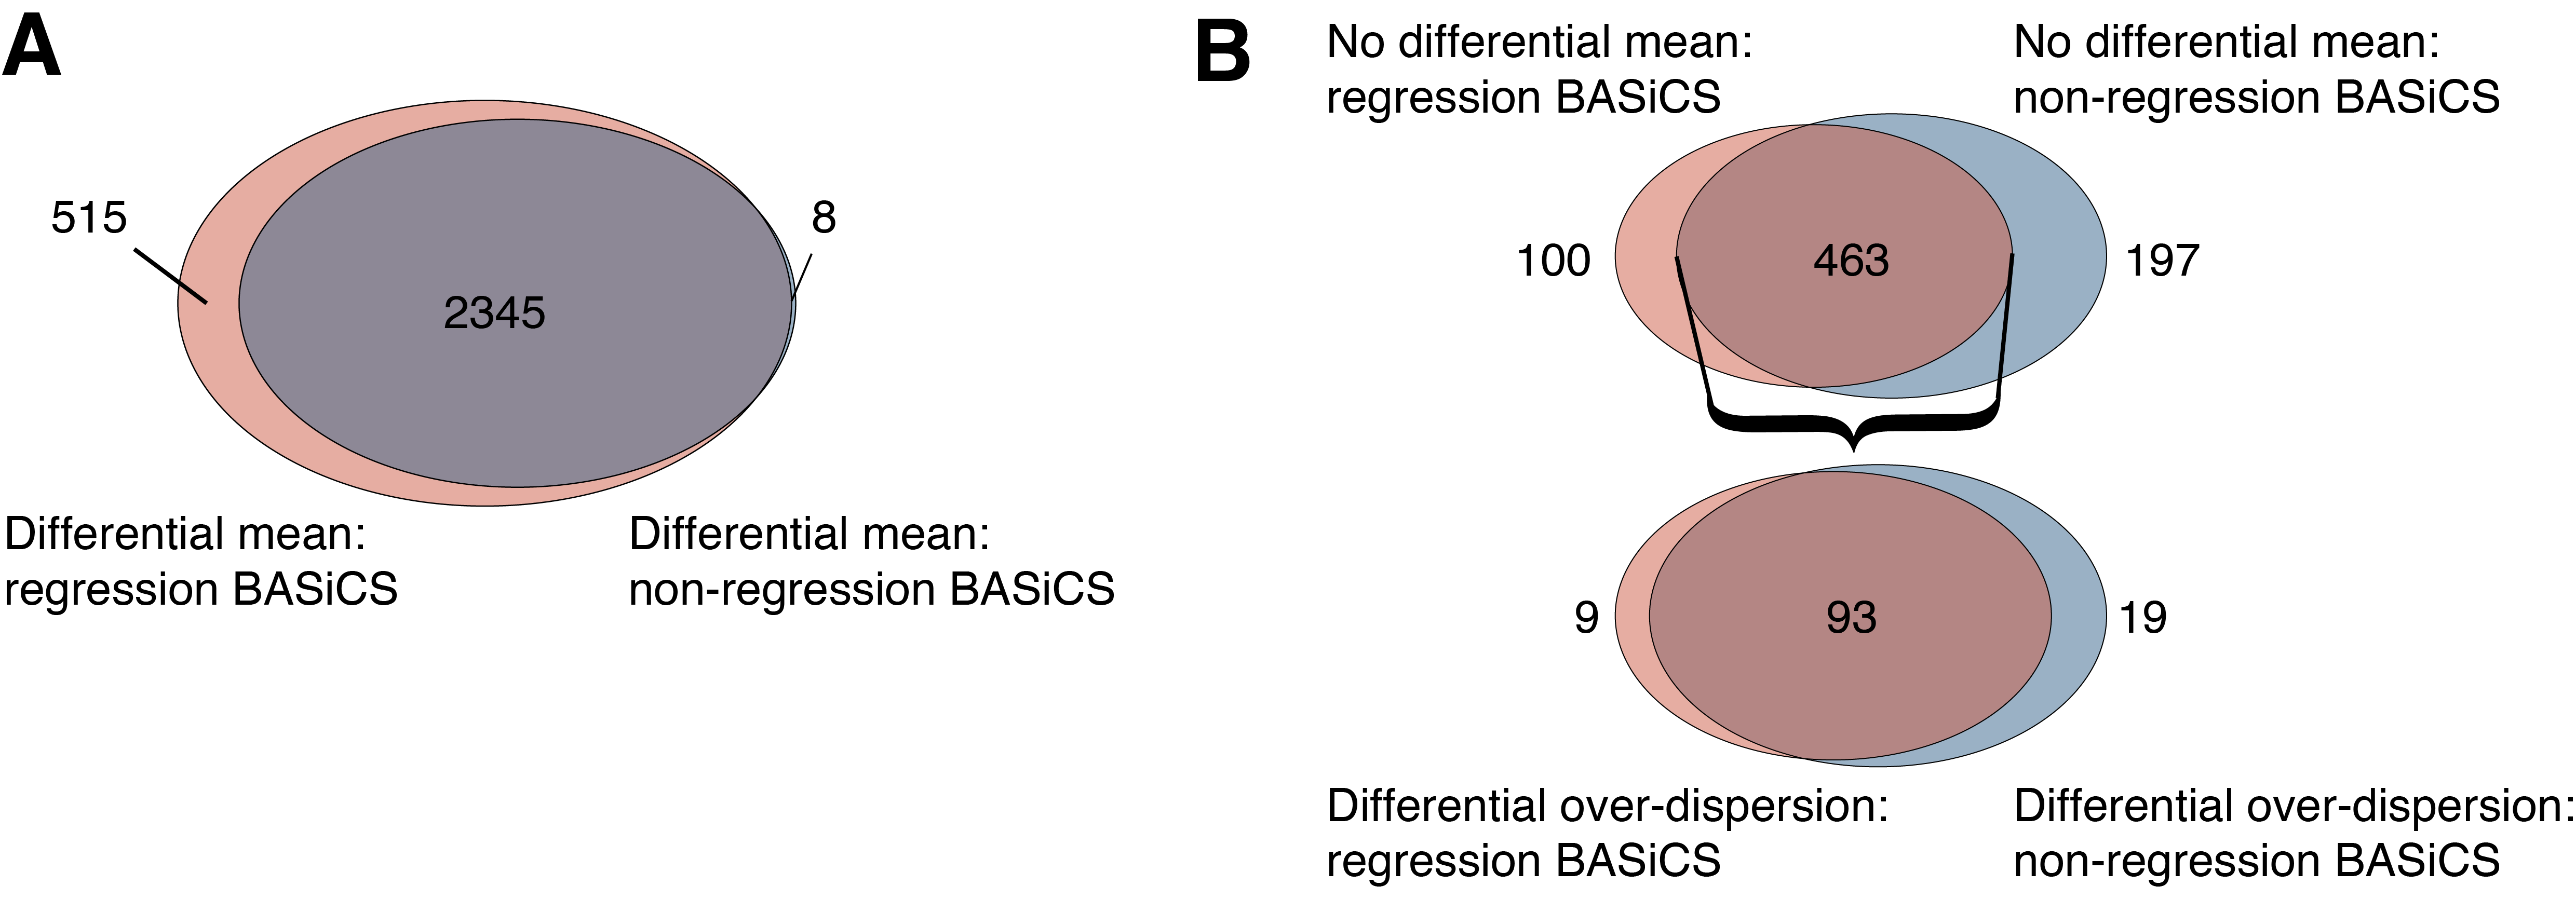
\includegraphics[width=\textwidth]{Fig_9.png}
\caption[Transcriptional dynamics and chromatin remodelling during spermiogenesis]{\textbf{Transcriptional dynamics coupled to chromatin remodelling during spermiogenesis (full legend on next page).}}
\label{fig3:spermiogenesis}
\end{figure}

\newpage

\captionsetup[figure]{list=no}
\addtocounter{figure}{-1}   
\captionof{figure}{\textbf{Transcriptional dynamics coupled to chromatin remodelling during spermiogenesis (continued).}\\
\textbf{(A)} Scaled normalized expression of histone variants (H1, H2A, H2B, H3), canonical histones, transition proteins (Tnp) and protamines (Prm) during spermiogenesis. Cells were ordered based on their developmental trajectory ranging from round spermatids (S1-S8) to elongating spermatids (S9-S14). \textbf{(B)} Expression of \textit{H3f3a} (middle panel) and \textit{H3f3b} (right panel) across the different germ cell populations. The panels show the expression of these genes in form of boxplots. \textbf{(C)} Similar visualization as in (A) of \textit{Hist1h4a} expression across germ cells. \\}
\captionsetup[figure]{list=yes}

For testis-specific histone variants, we observed highest expression in elongating spermatids, with most variants increasing strongly in expression from S5 onwards. While some variants had a consistently high expression level, \textit{Hils1} and \textit{H1fnt} decreased in expression towards the late stages, similarly to \textit{Tnp1} and \textit{Tnp2} \citep{Zhao2004}. Both histone variants are important for male fertility, and \textit{Hils1} has previously been shown to interact with \textit{Tnp1} \citep{Tanaka2005}. In contrast, three testis-specific histone variants \textit{Hypm}, \textit{H2afb1} and \textit{H2bl1} (\textit{1700024p04rik}) showed consistently high expression until the end of differentiation similar to protamines, suggesting these variants contribute to the final genome condensation.\\

As a consequence of chromatin condensation, transcription ceases in spermatids at the round to elongating switch, consistent with the lack of active RNA Pol II at S10 and later stages \citep{Dottermusch‐Heidel2014}. Our data clearly reflect this transcriptional shut-down since the number of expressed genes is stable until approximately S9 before gradually declining \textbf{(Fig. \ref{fig3:transcriptional_shutdown}A)}.
In the 8 days following transcriptional shut-down, spermatids still need to undergo drastic morphological changes, including the assembly of sperm-specific structures such as the flagellum, before mature testicular sperm can be released into the lumen \citep{ODonnell2014}. To achieve this in the absence of active transcription, spermatids store large amounts of mRNAs in a perinuclear RNA granule termed the chromatoid body or \emph{nuage} \citep{Kotaja2007}. RNA stored in the chromatoid body is then released for translation, suggesting that these molecules may play vital roles during late stages of spermiogenesis. However, identifying the RNAs that are stored has been hindered by difficulties in purifying late spermatids. \\

By correlating normalized gene expression against the number of genes expressed, we identified a large number of genes that gradually decrease in relative expression after transcriptional shut-down, the timing of which could be indicative of RNA degradation rates. We reasoned that transcripts where the relative expression after transcriptional shut-down appeared to increase are likely protected from degradation \textbf{(Fig. \ref{fig3:transcriptional_shutdown}B)}. This included genes with well-known spermiogenesis-specific functions; indeed, transition proteins and protamines are involved in chromatin condensation, as well as genes involved in sperm motility such as \textit{Akap4} and \textit{Cabs1} \citep{Kawashima2009, Miki2002}. This gene set is therefore a resource for identification of novel spermiogenesis-related proteins with potential roles in fertility.

\begin{figure}[!h]
\centering
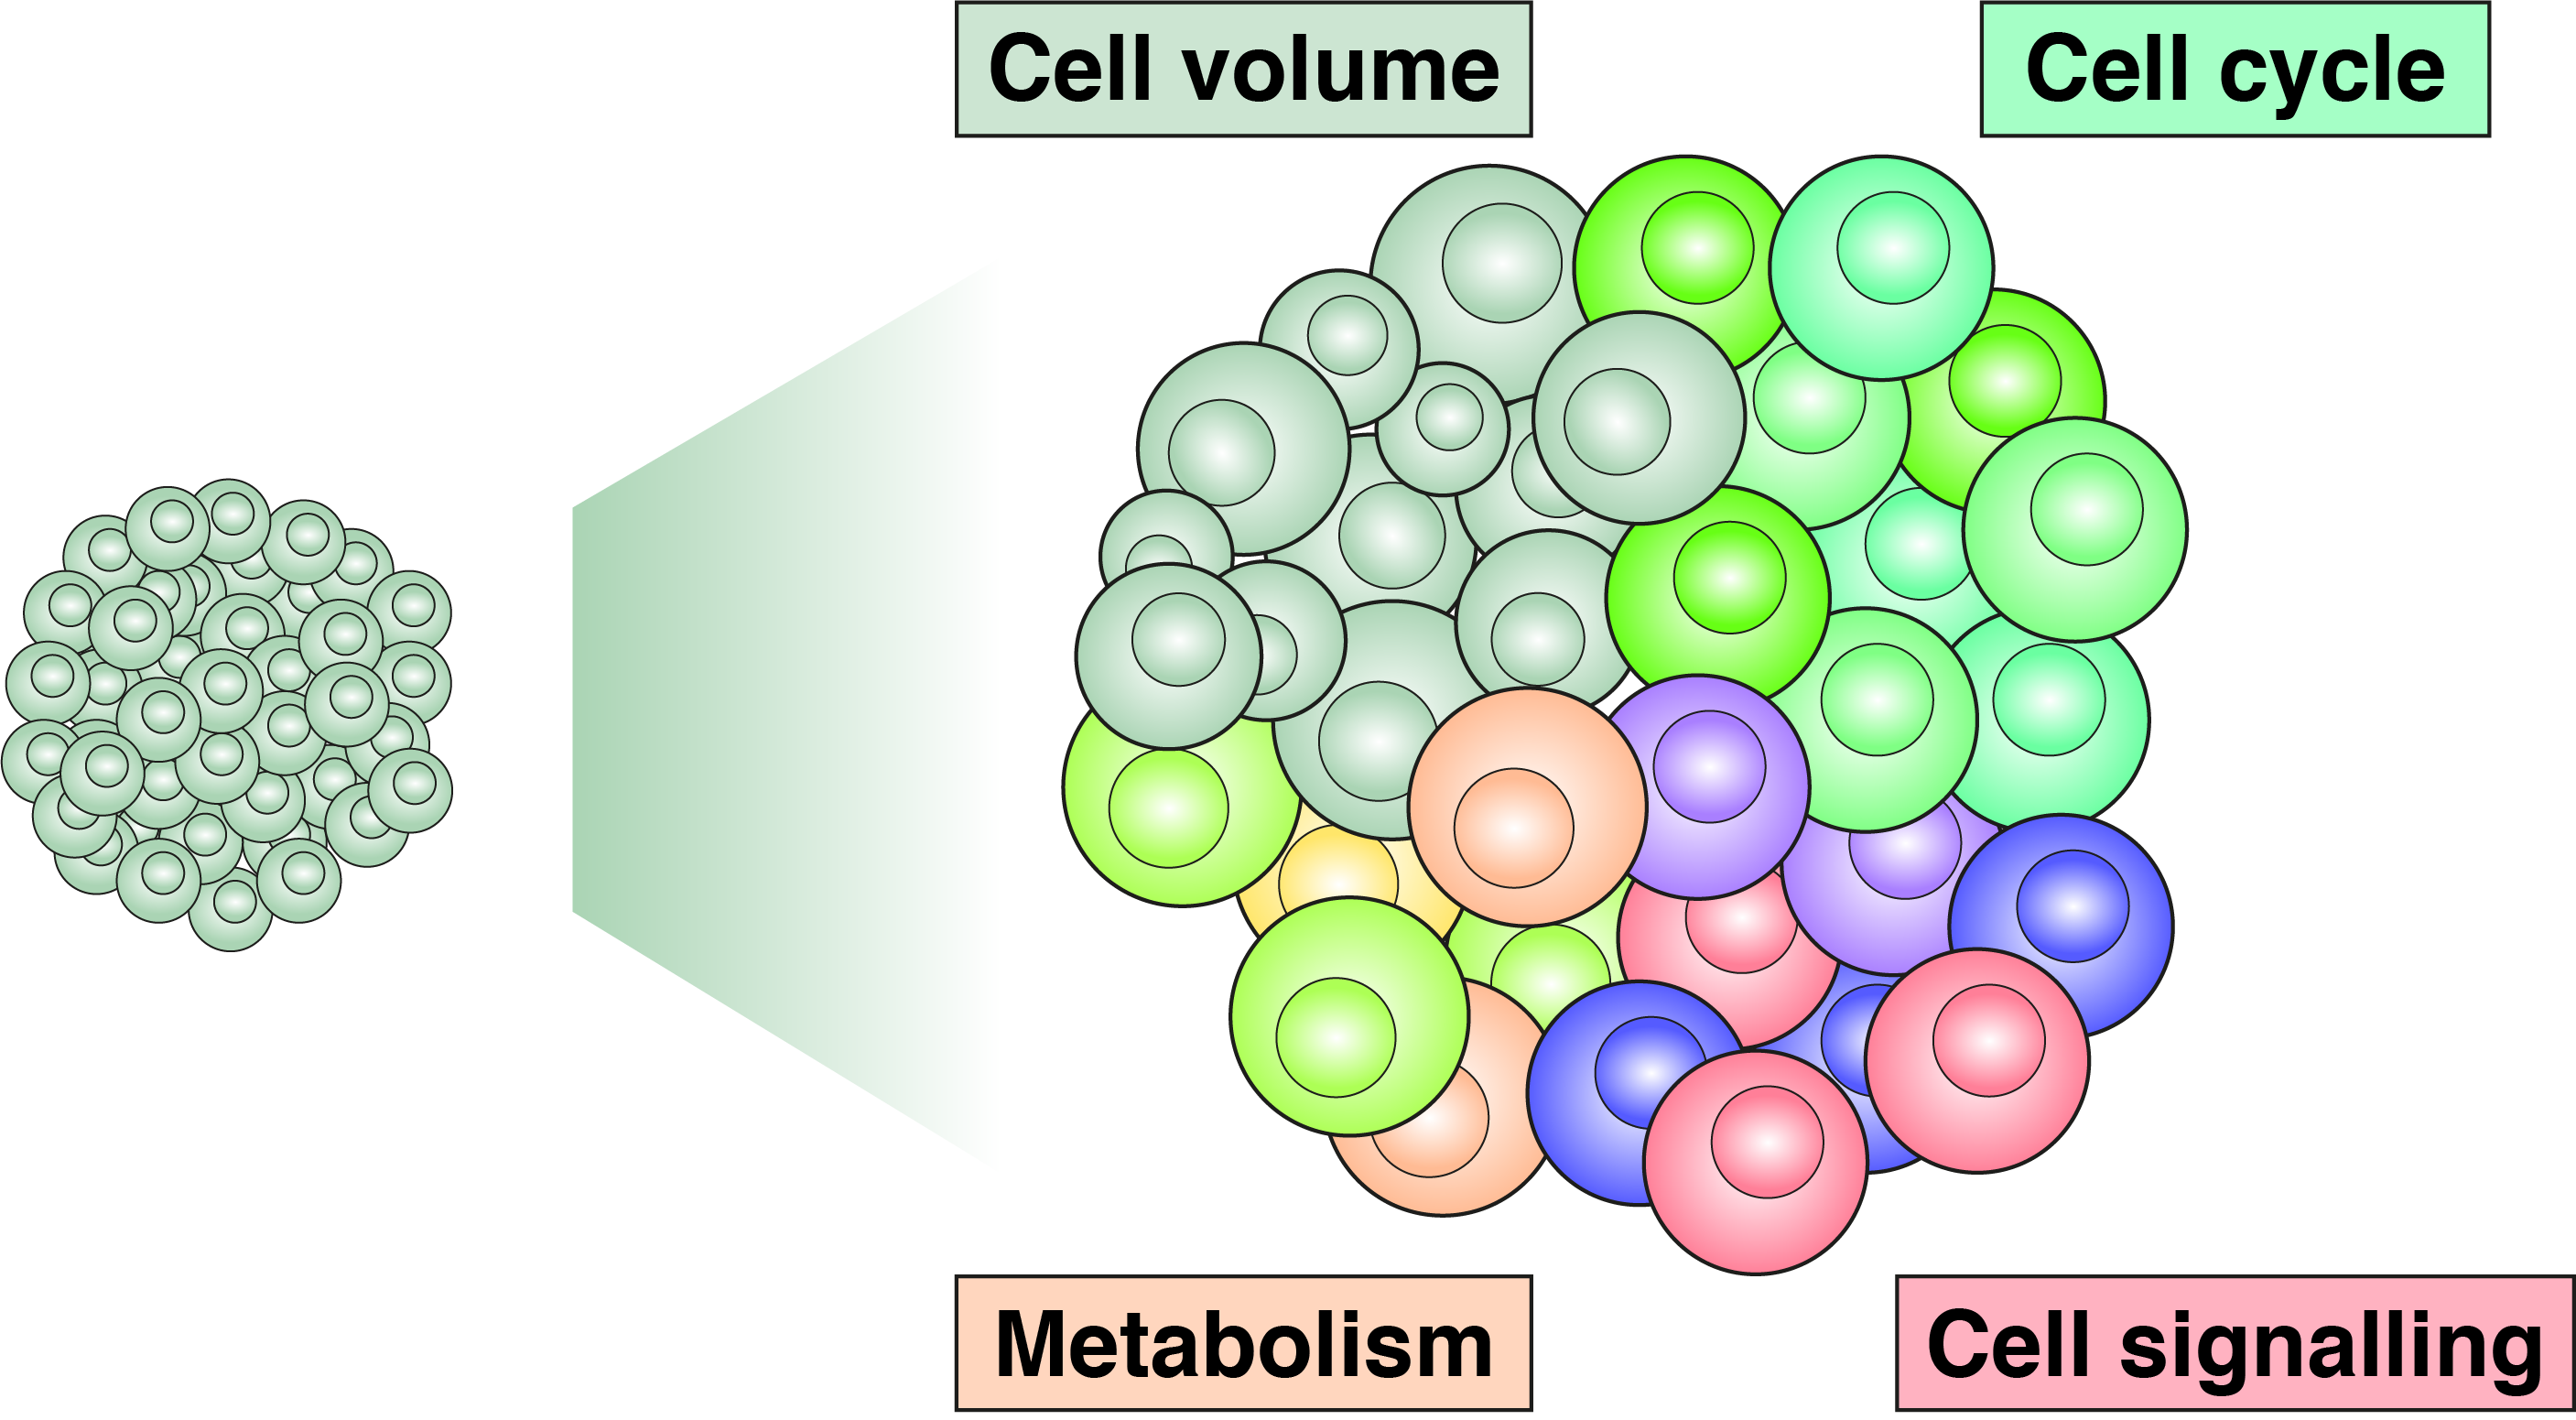
\includegraphics[width=\textwidth]{Fig_10.png}
\caption[Transcriptional shut-down during spermiogenesis]{\textbf{Transcriptional shut-down during spermiogenesis.} \\
\textbf{(A)} Number of genes expressed per spermatid. Cells were ordered based on their developmental trajectory. Red line indicates a smooth regression (loess) fit. \textbf{(B)} For each gene, its normalised expression per cell was correlated with the number of genes expressed per cell. Genes were ordered based on the correlation coefficient and grouped into 9 sets. Scaled expression was averaged across genes within each gene set. Vertical dashed line indicates transcriptional shut-down between S9 and S10.}
\label{fig3:transcriptional_shutdown}
\end{figure}

\section{Meiotic silencing dynamics of sex chromosomes}

A male-specific feature of meiosis is the transcriptional silencing of sex chromosomes, followed by partial reactivation in post-meiotic spermatids. This process is termed meiotic sex chromosome inactivation (MSCI), and is caused by asynapsis of the sex chromosomes, leading to accumulation of phosphorylated H2AFX and the formation of the sex body \citep{Hamer2003} \textbf{(Fig. \ref{fig3:X_reactivation}A)}. 

\newpage

\begin{figure}[!h]
\centering
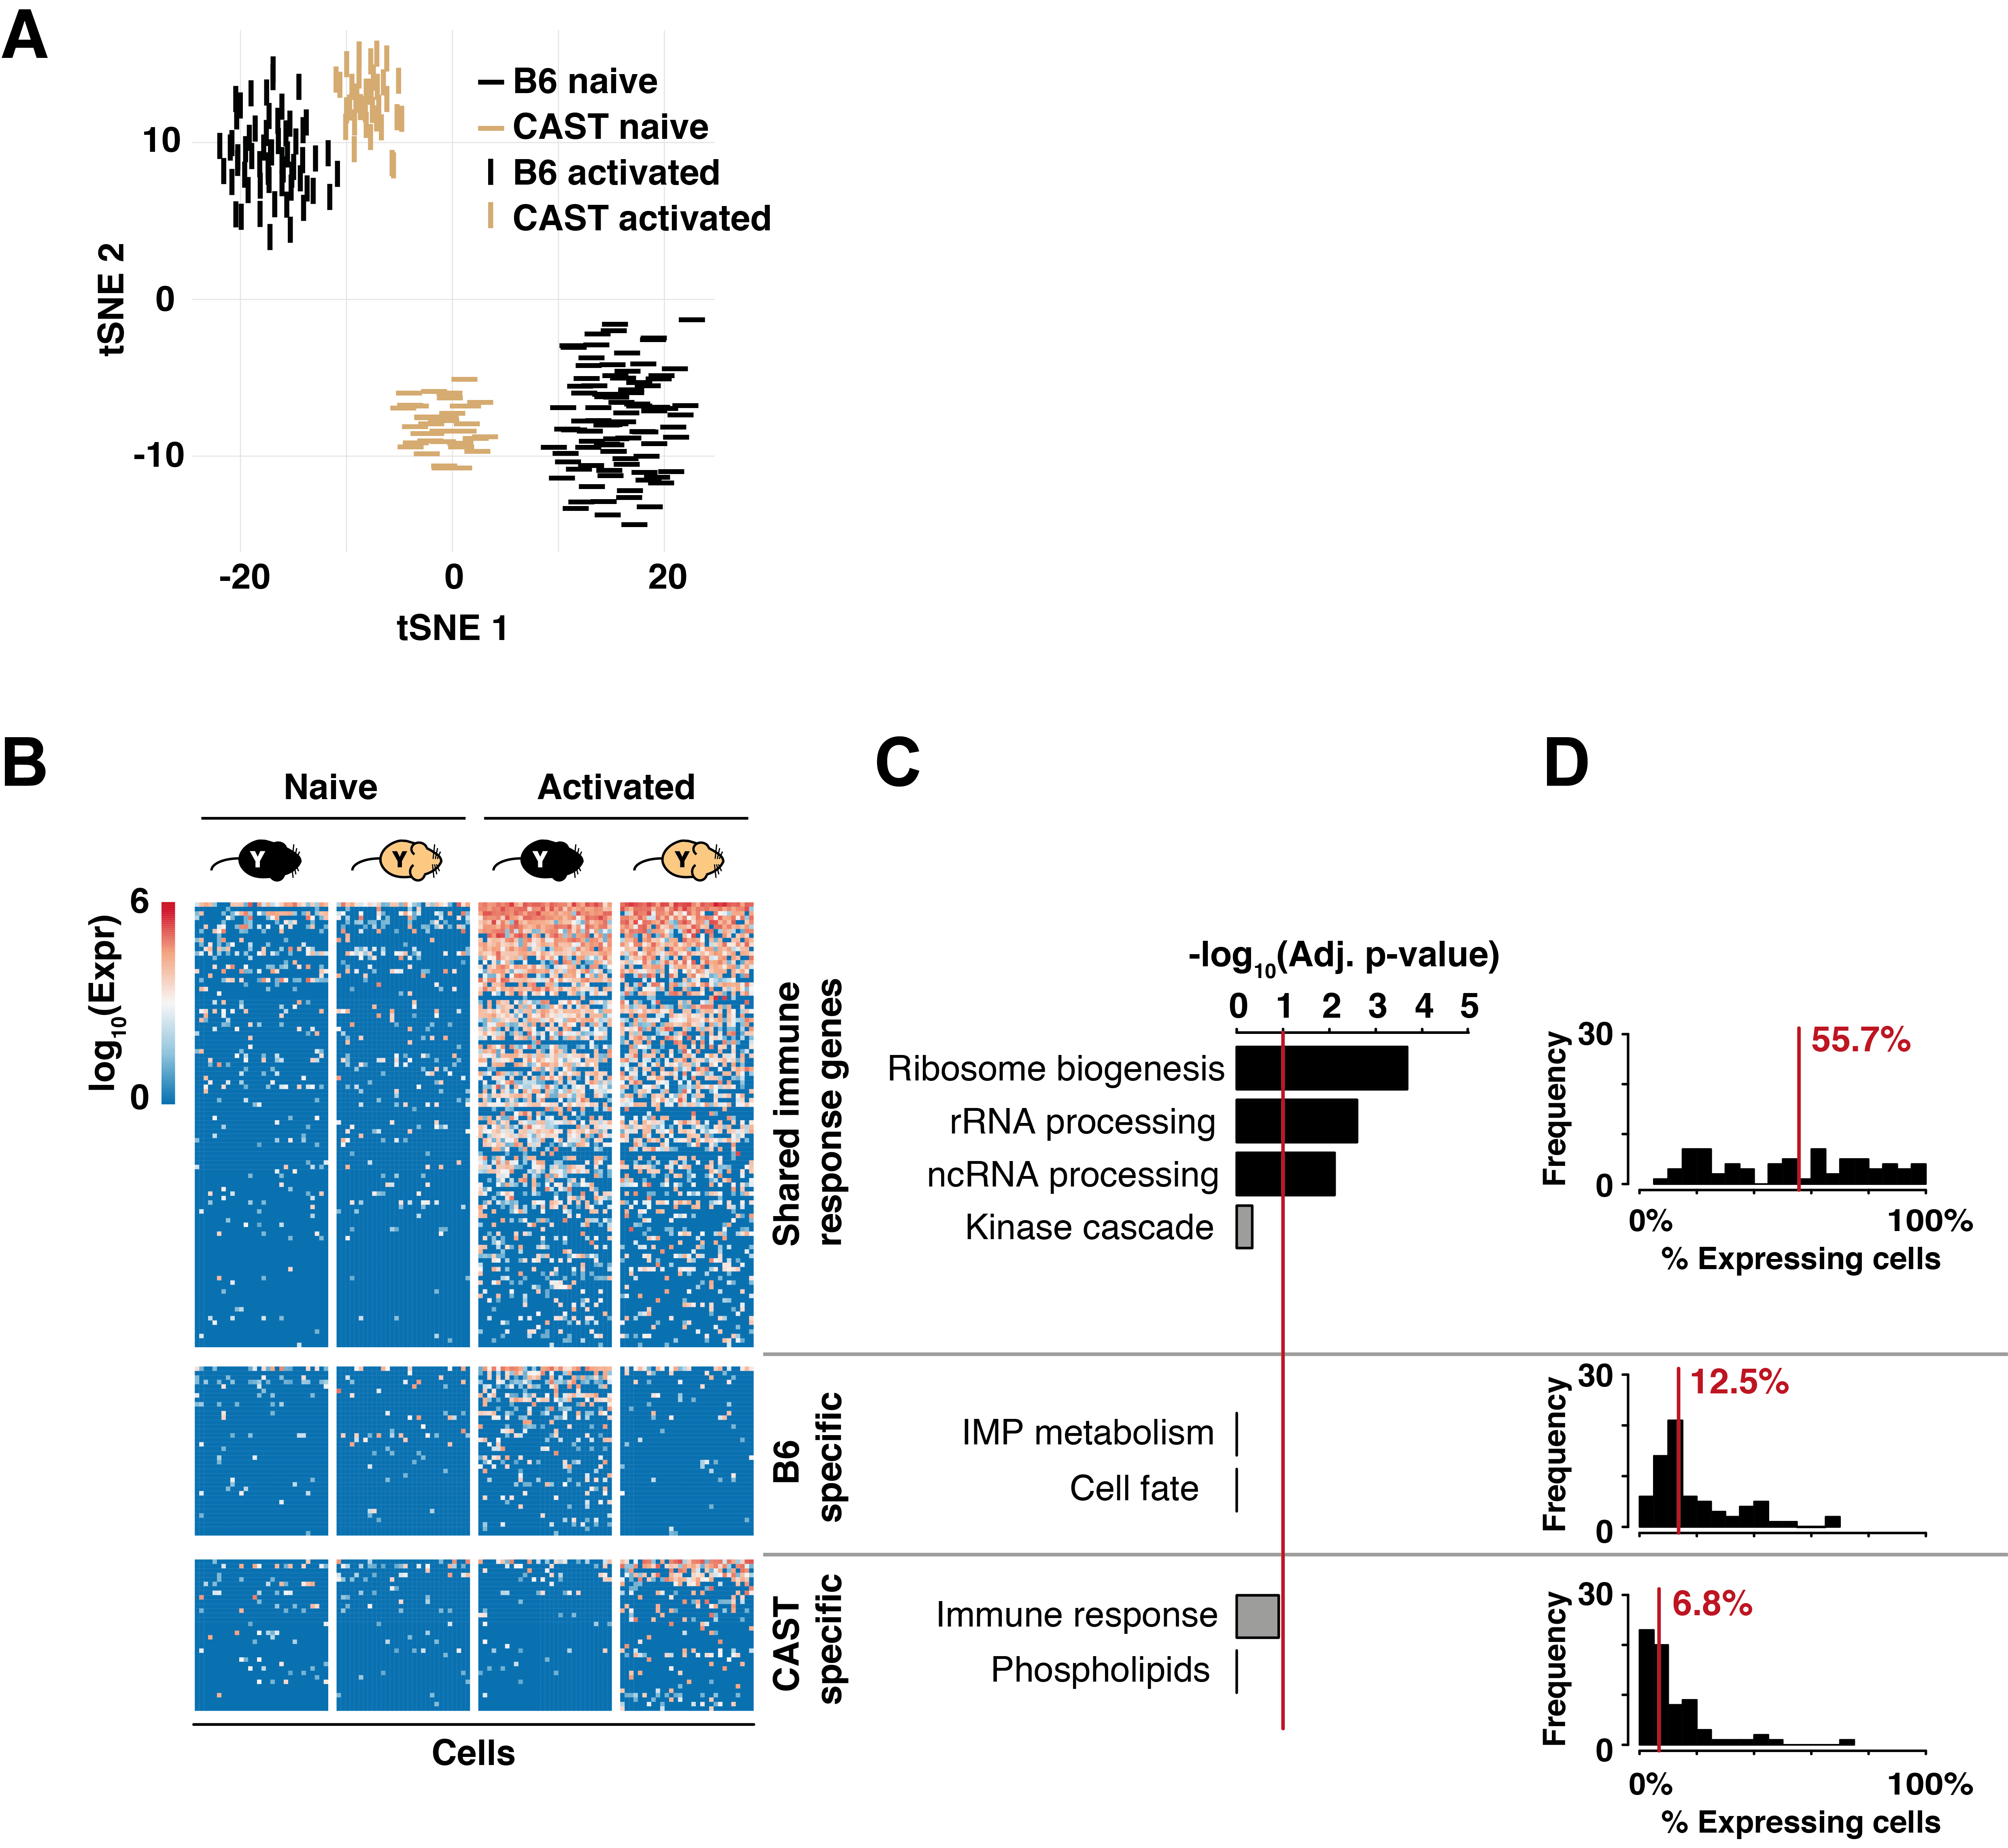
\includegraphics[width=\textwidth]{Fig_11.png}
\caption[X chromosome dynamics during spermatogenesis]{\textbf{X chromosome dynamics during spermatogenesis.} \\
\textbf{(A)} Schematic of sex chromosome sub-nuclear localisation through spermatogenesis. \textbf{(B)} For each cell, the ratio of mean expression of genes on Chr 9, Chr X and Chr Y to the mean expression of genes across all autosomes is represented as a boxplot for cells allocated to each developmental stage. SG – spermatogonia, M – metaphase. \textbf{(C)} Expression of all X chromosome genes (> 10 average counts) in bulk RNA-Seq data across the juvenile time course. Columns correspond to developmental stage and rows are ordered by the log$_2$ fold change between spermatocytes (stages before postnatal day (P) 20) and spermatids (stages after and including P20). Horizontal dashes indicate genes that are targets of \textit{Rnf8} (green) and \textit{Scml2} (blue) \citep{Adams2018}. \textbf{(D)} Average expression of spermatid specific genes (panel (C)) per germ cell type. Columns are ordered by developmental stage and rows are ordered by peak gene expression through development. Multi-copy genes are highlighted in bold.}
\label{fig3:X_reactivation}
\end{figure}

\newpage

We computed the ratio of expression from the X, Y chromosome and chromosome 9 to all autosomes. For this, we selected genes that were expressed in more than 30\% of spermatogonia or 30\% of spermatids, the cell types with detectable sex chromosome expression. For each cell, the mean expression across these genes per chromosome was calculated. Mean expression of the chromosomes of interest (9, X and Y) was divided by mean expression of the autosomes. By plotting the ratio of gene expression from the X or Y chromosomes compared to all autosomes, the inactivation and re-activation status of the sex chromosomes can be deduced \textbf{(Fig. \ref{fig3:X_reactivation}B)}. The X chromosome is partially upregulated in spermatogonia as described by Sangrithi \emph{et al.} (X:A ratio < 1) \citep{Sangrithi2017}, followed by transcriptional silencing in spermatocytes. Throughout spermiogenesis, expression from the X gradually increases, reaching X:A ratios comparable to spermatogonia, therefore suggesting a substantial reactivation of the X chromosome in post-meiotic spermatids. \\

Transcriptional silencing was originally thought to persist throughout post-meiotic development \citep{Greaves2006, Turner2006}; however, several genes have been shown to be re- or \emph{de novo} activated in spermatids, some of which are dependent on \textit{Rnf8} (Ring finger protein 8) and/or \textit{Scml2} (Sex comb on midleg-like 2) \citep{Hasegawa2015, Sin2012, Sin2015}. However, the precise timing and order of the transcriptional reactivation of \emph{de novo} escape genes during spermiogenesis has not been explored. \\
Profiling whole-testis transcriptomes of juvenile mice sampled every two days during the first wave of spermatogenesis allowed the sensitive detection of spermatid-specific escape genes \textbf{(Fig. \ref{fig3:cell_staging}A)}. Due to the gradual emergence of germ cell types during the first spermatogenic wave, differential expression analysis between early (< P20) and late (> P20) time points revealed genes exclusively expressed in spermatids and which are thus \emph{de novo} activated escape genes (n = 128) \textbf{(Fig. \ref{fig3:X_reactivation}C)}. These include many of the previously annotated escape genes such as \textit{Cypt1}, \textit{Cycl1}, and \textit{Akap4}, and show an enrichment for genes dependent on \textit{Rnf8} or \textit{Scml2} for reactivation in spermatids (Fisher's Exact Test: \textit{Rnf8}-targets, p-value < 5x10-12; \textit{Scml2}-targets, p-value < 2x10-9) \textbf{(Fig. \ref{fig3:X_reactivation}C)} \citep{Adams2018}. 

\newpage

\section{Epigenetic mechanisms underlying \emph{de novo} escape gene activation}

To gain insight into the mechanisms underlying de novo activation of spermatid-specific escape genes on the X chromosome, we profiled the chromatin landscape in spermatocytes and spermatids using the newly developed CUT\&{}RUN protocol for low cell numbers \textbf{(Fig.~\ref{fig3:K9_global}A and Appendix \ref{appA.2})} \citep{Skene2018}. \\

\textbf{CUT\&{}RUN computational analysis}
Reads were aligned to the Mus musculus genome (GRCm38) using \textit{Bowtie2} with the following settings: --local --very-sensitive-local --no-unal -q --phred33. Paired end reads were counted in specified regions using the \textit{regionCounts} function implemented in the \textit{csaw} Bioconductor package \citep{Lun2015}. For this, duplicated reads, reads mapped more than 1000 bp apart and reads mapping to blacklisted regions (available at: http://mitra.stanford.edu/kundaje/akundaje/release/blacklists/mm10-mouse/mm10.blacklist.bed.gz) were removed. Regions of interests were: promoters (obtained using the \textit{promoters} function of the \textit{GenomicFeatures} package), 1000 bp windows across the chromosome (using the \textit{windowCounts} function of \textit{csaw}) and whole chromosomes. Counts per region were normalized based on library size (counts per million, CPM) for promoter regions and 1000 bp windows; additionally, when considering entire chromosomes, the length of the chromosome was accounted for by computing the Fragments per Kilobase per Million mapped reads (FPKMs). 

We assayed trimethylation of histone H3 on lysine 4 (H3K4me3) as a proxy for promoter activity, as well as repressive trimethylation of lysine 9 (H3K9me3), which is associated with the sex body in early and late spermatocytes and enriched in post-meiotic sex chromatin (PMSC) \citep{Greaves2006, Tachibana2007}. By profiling the enrichment of H3K9me3 across all chromosomes, we confirmed that the X chromosome has high levels of H3K9me3 in spermatids \citep{Moretti2016}. In addition, we now show that H3K9me3 accumulation begins earlier in meiosis, and indeed spermatocytes show enrichment of this repressive mark \textbf{(Fig.~\ref{fig3:K9_global}B)}. 

\begin{figure}[!h]
\centering
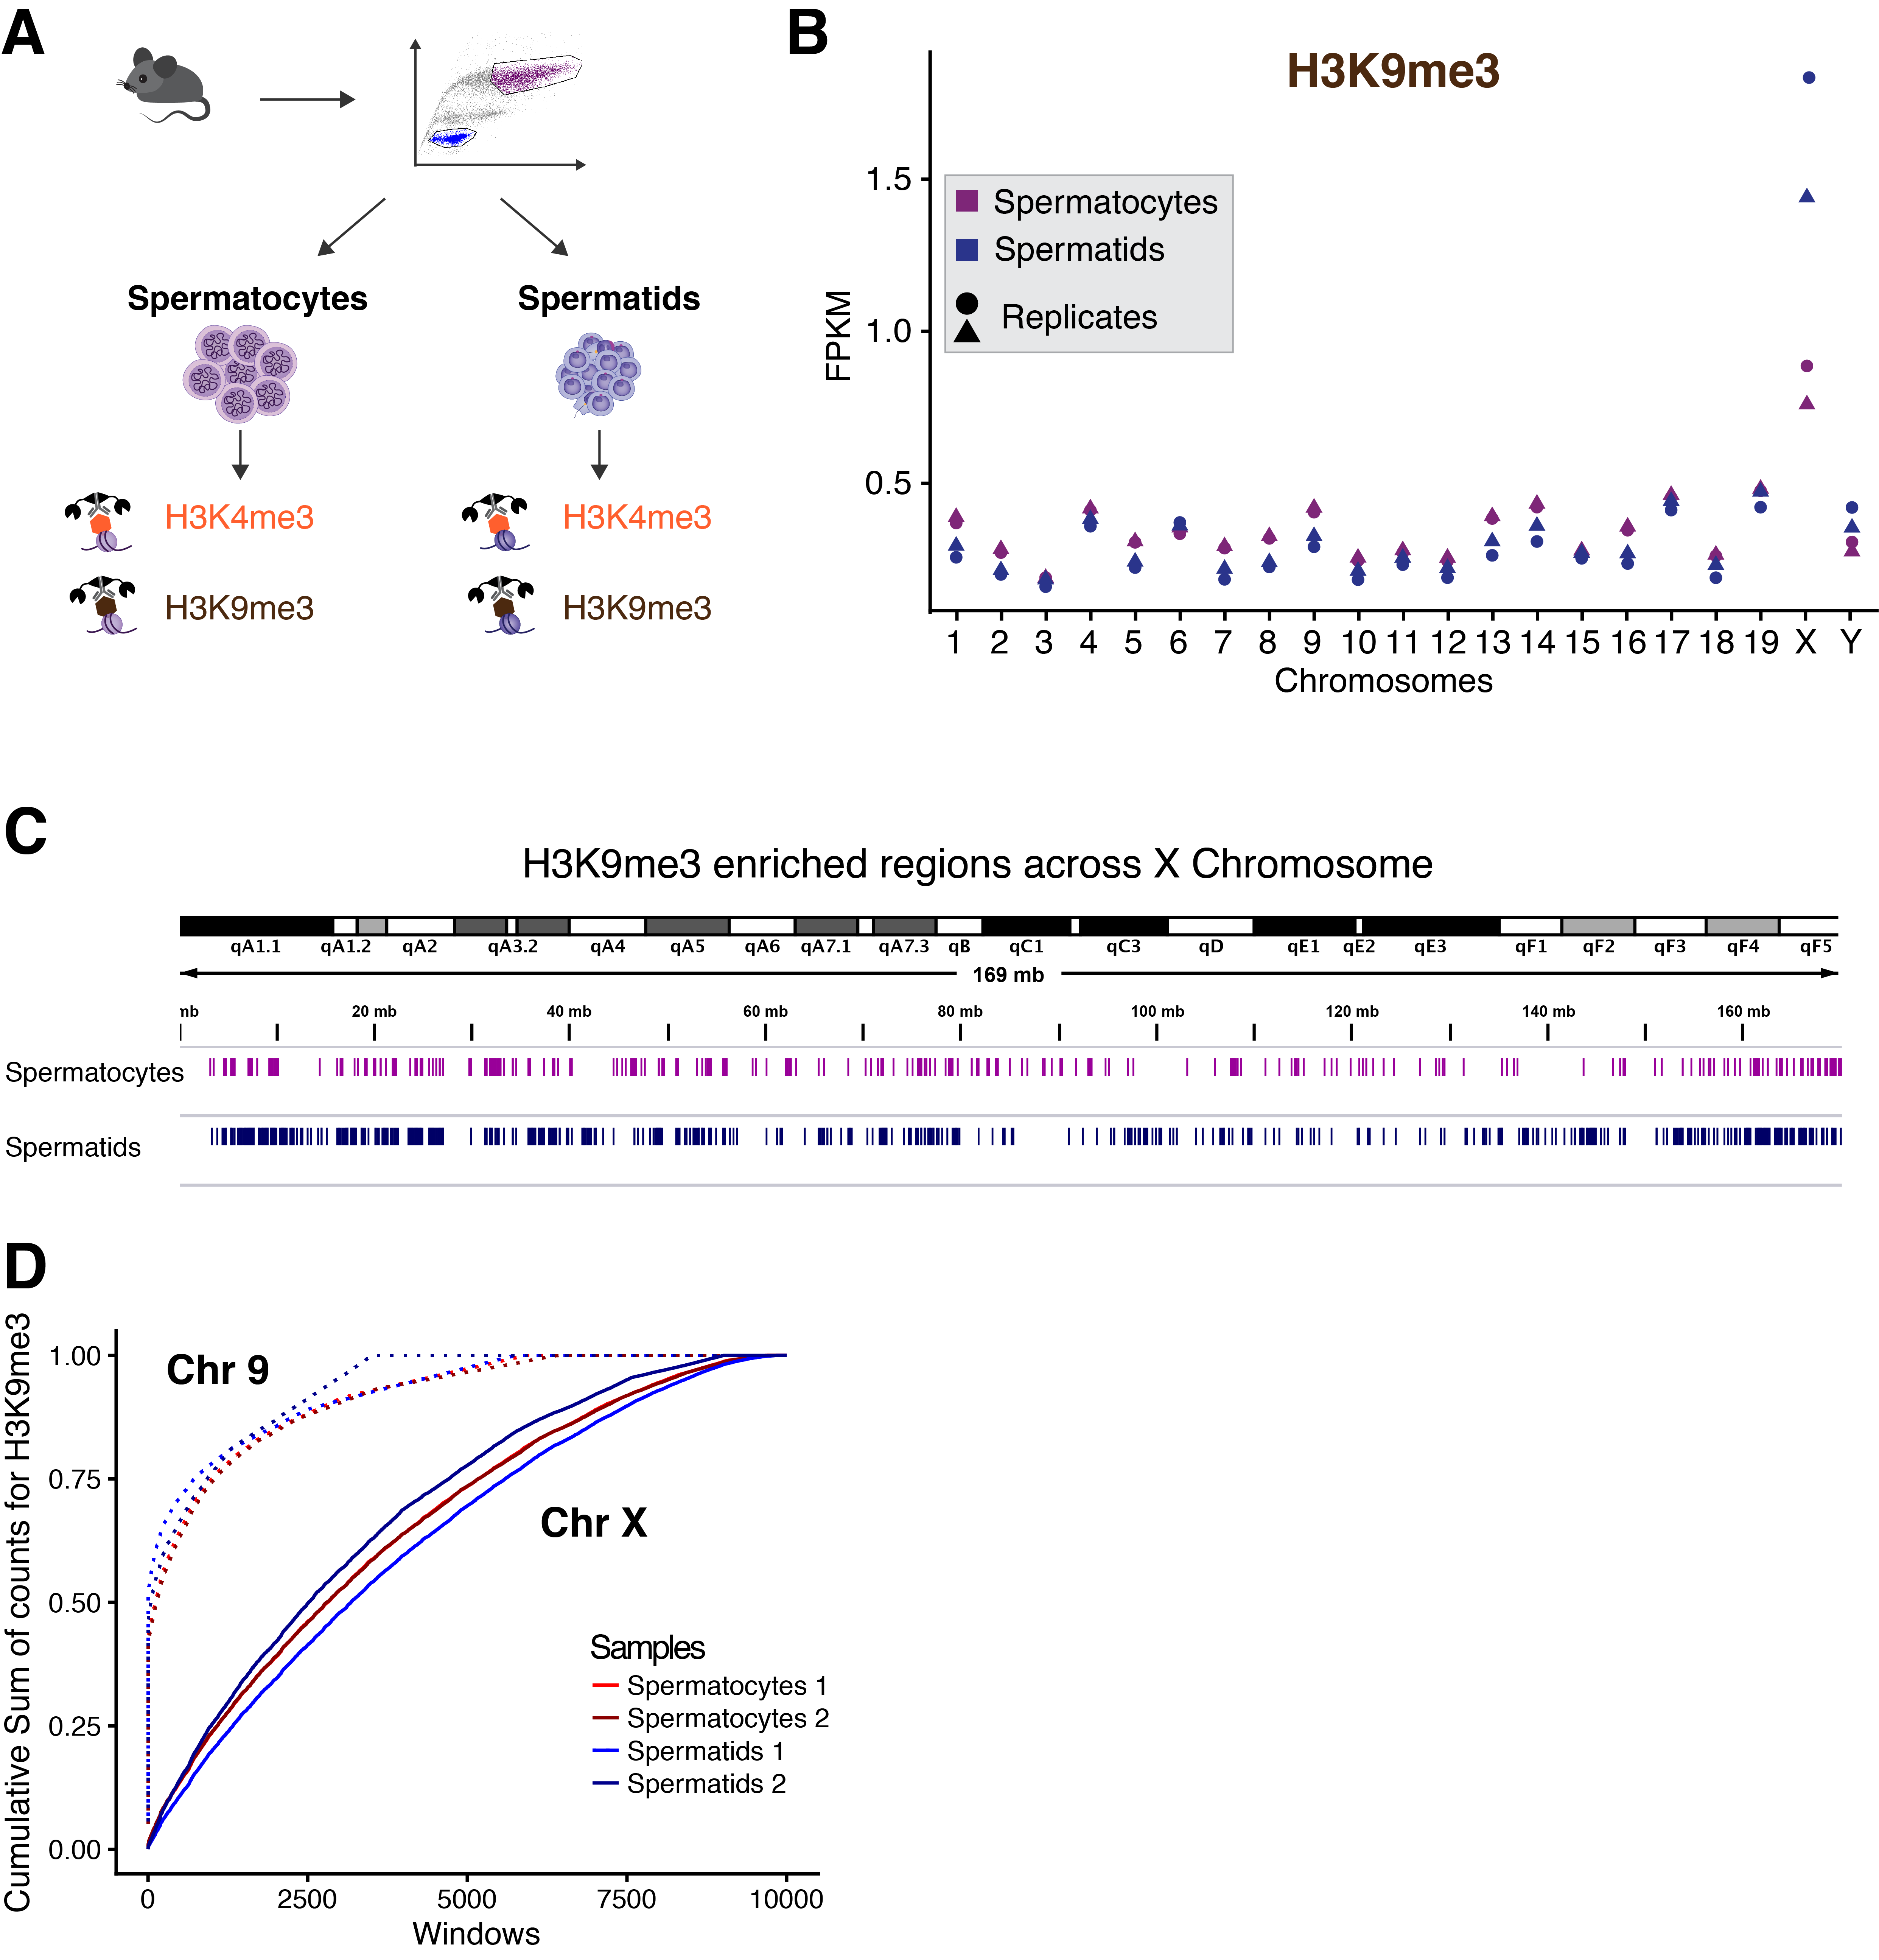
\includegraphics[width=0.8\textwidth]{Fig_12.png}
\caption[Chromatin profiling in spermatocytes and spermatids]{\textbf{Profiling of repressive and active chromatin marks in spermatocytes and spermatids.} \\
\textbf{(A)} Spermatocytes and spermatids were isolated from the same individual using FACS and profiled using H3K4me3 (active mark) and H3K9me3 (repressive mark) using CUT\&{}RUN. \textbf{(B)} Number of H3K9me3 Fragments Per Kilobase per Million (FPKM) for each chromosome. Pink (spermatocytes); Blue (spermatids). Shape corresponds to biological replicate. \textbf{(C)} The top 1000 windows with highest H3K9me3 signal (1000 bp width, CPM) were merged using a tolerance of 1500 bp. Representative tracks of one replicate in spermatocytes and one replicate in spermatids are shown. \textbf{(D)} Cumulative summed counts per million across 10000 randomly sampled windows (1000 bp width) visualizing the distribution of the H3K9me3 signal across chromosome 9 (dashed line) and chromosome X (solid line). 
}
\label{fig3:K9_global}
\end{figure}

On autosomes, H3K9me3 is enriched in pericentromeric regions of constitutive heterochromatin \citep{Peters2001}; in sharp contrast, this repressive histone mark is more evenly distributed across the X chromosome in spermatocytes  \textbf{(Fig.~\ref{fig3:K9_global}D)}. Nevertheless, we detected broad regions showing particularly high levels of H3K9me3 scattered across the X chromosome  \textbf{(Fig.~\ref{fig3:K9_global}C)}, including the promoter of \textit{Akap4}, a well-known escape gene. This discovery prompted us to profile the chromatin dynamics of active and repressive marks at promoters of \emph{de novo} escape genes (\emph{spermatid-specific genes}) versus the promoters of all other expressed X-chromosome genes (\emph{non-spermatid specific genes}) \textbf{(Fig.~\ref{fig3:X_reactivation}C)}.

\begin{figure}[!h]
\centering
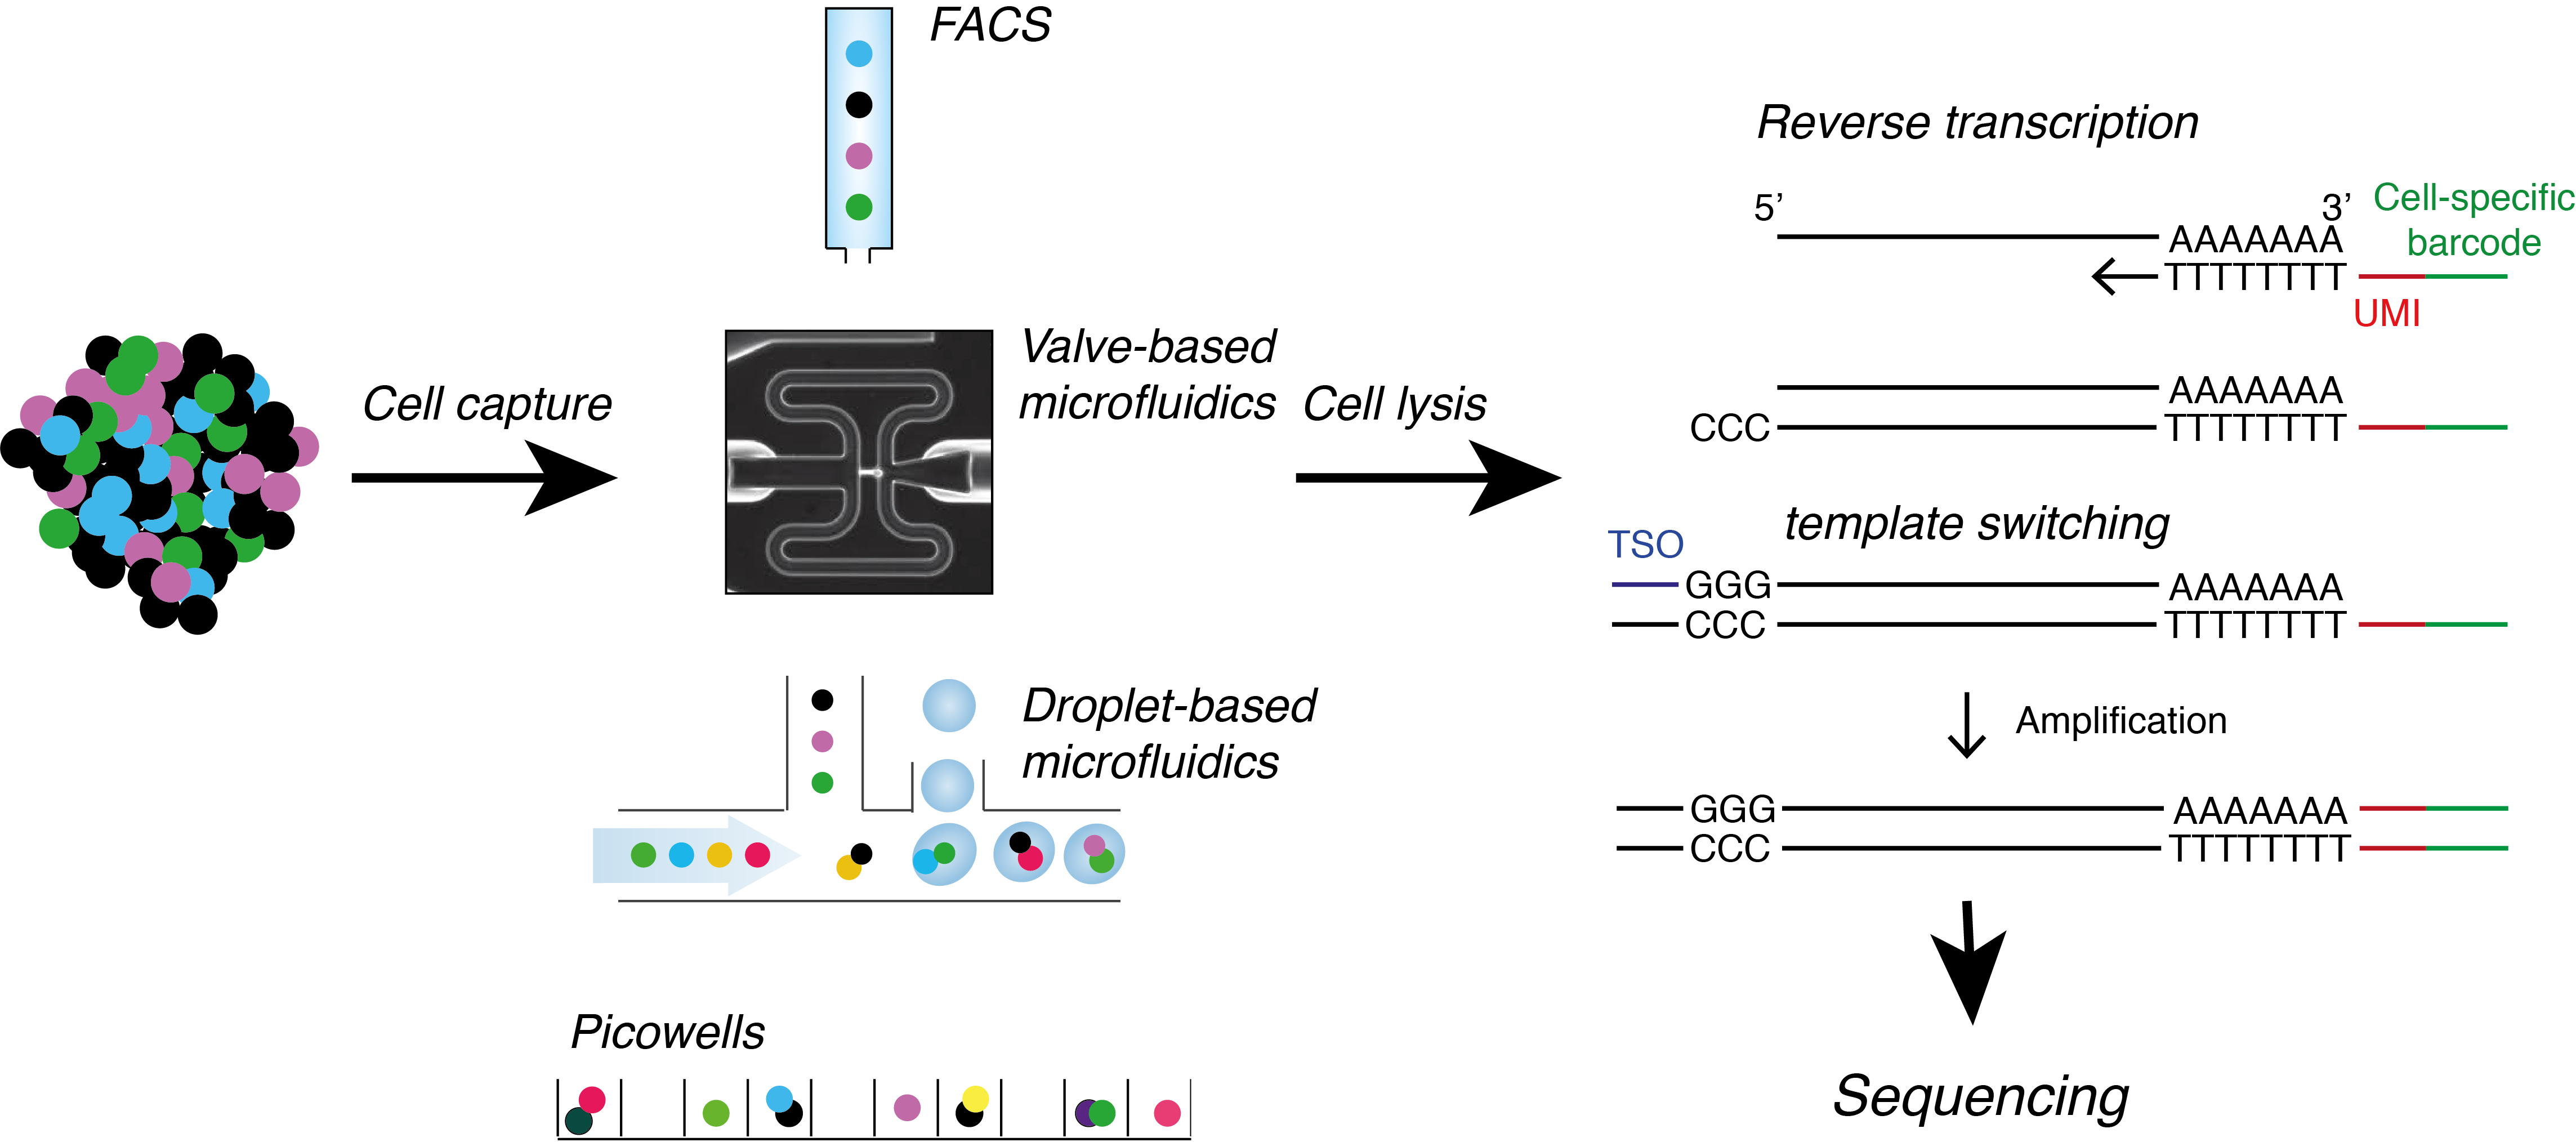
\includegraphics[width=\textwidth]{Fig_13.png}
\caption[Targeted repression of spermatid-specifc escape genes in spermatocytes]{\textbf{Targeted repression of spermatid-specifc escape genes in spermatocytes.} \\
\textbf{(A)} and \textbf{(B)} Boxplot of H3K4me3 (A) and H3K9me3 (B) Counts Per Million (CPM) in promoter regions of spermatid specific (n=127) and non-spermatid specific (n=617) genes for spermatocytes (left) and spermatids (right).  \# indicates statistical significance (Wilcoxon-Mann-Whitney: p-value < 1x10$^{-10}$), n.s. – not significant. 
(E) Genome tracks of H3K4me3 and H3K9me3 for two representative spermatid-specific genes (\textit{Akap4} and \textit{Cypt1}) for spermatocytes (left) and spermatids (right). Reads were scaled by library size.}
\label{fig3:K9_K4_targeted}
\end{figure}

In spermatocytes, spermatid-specific genes showed lower enrichment in H3K4me3 than non-spermatid specific genes (Wilcoxon-Mann-Whitney: p-value < 2.2x10$^{-16}$) \textbf{(Fig.~\ref{fig3:K9_K4_targeted}A, left panel)}. In contrast, spermatid-specific genes have on average elevated H3K4me3 in spermatids, as expected based on their increased expression level compared to spermatocytes \textbf{(Fig.~\ref{fig3:K9_K4_targeted}A, right panel)}. When examining the deposition of H3K9me3 on the promoters of X-linked genes, we detected a strong enrichment in spermatid-specific escape genes in spermatocytes (Wilcoxon-Mann-Whitney: p-value < 3.7x10$^{-11}$) \textbf{(Fig.~\ref{fig3:K9_K4_targeted}B)}. This pattern indicates that spermatid-specific genes are more strongly repressed in spermatocytes. \\

Our results describe for the first time, the precise epigenetic changes associated with escape gene activation in post-meiotic cells. These dynamics are exemplified by the chromatin remodelling that occurs around \textit{Akap4} and \textit{Cypt1}, both of which are well-studied spermatid-specific genes \textbf{(Fig.~\ref{fig3:K9_K4_targeted}C)}. The promoters of these genes have high levels of H3K9me3 in spermatocytes, which decreases in spermatids, while H3K4me3 levels are strongly increased. 

\section{Measuring changes in variability over pseudo-time}

As described above, spermatogenesis is a unidirectional and continuous differentiation process coupled to a complex system of developmental steps. In this section, I will apply the regression BASiCS model developed in the previous chapter to study changes in transcriptional variability over the time-course of spermatogenesis. In mouse hematopoietic cell differentiation,  cell-to-cell diversity increases at critical state transitions where cell fate decisions are made \citep{Mojtahedi2016}. A similar effect was seen in chicken erythroid progenitor cells where the Shannon entropy is highest directly at the point of fate commitment and declines during the irreversible commitment to differentiation \cite{Richard2016}. In the previous chapter, we have demonstrated that transcriptional variability shows dynamic changes during CD4\plus{} T cell differentiation with high variability being observed at a possible early commitment point and a decrease in variability upon proliferation. Here, I profile changes in variability for individual genes during spermiogenesis, the differentiation process that directly follows meiosis (see \textbf{Section \ref{sec3:spermiogenesis}}). As described above, spermiogenesis is a differentiation process that involves an extensive remodelling of the chromatin with transcriptional shut-down occurring at around spermatid stage S10. I therefore selected spermatids from stages S1 to S9 for analysis where transcriptional regulation is needed for sperm maturation. Transcriptional changes after S10 are only due to degradation of mRNA. 

\subsection{Using BASiCS on continuous data}

Modelling changes in mean expression over a differentiation time-course is done by ordering transcriptional profiles of individual cell along their so called \emph{pseudo-time}. Different methods have been proposed to perform this ordering based on minimum spanning trees \citep{Trapnell2014} and nearest-neighbour graphs \cite{Setty2016}, Gaussian Processes \citep{Reid2016a, Campbell2016b} and diffusion maps \citep{Haghverdi2016}. Once the pseudo-temporal ordering is determined, genes which change in expression over pseudo-time can be found by fitting a generalized linear model to the expression counts and performing a likelihood ratio test against a null model with no pseudo-time dependence \citep{Trapnell2014}. Profiling changes in variability is more complicated as no single-cell measures of variability are available. Here, I use BASiCS to estimate residual over-dispersion parameters for homogeneous cell populations along the differentiation time-course. Different ways of identifying those homogeneous populations exists. First, ordered cells can be split into populations of equal size (e.g.~200 cells per group). This approach produces heterogeneous cell populations when quick cell state transitions occur which leads to abrupt changes in expression. I therefore rely on the clustering performed in \textbf{Section \ref{sec3:clustering}} which splits the full cell population along the differentiation trajectory. For each cluster from S1 to S9, the regression BASiCS model was run for 40,000 iterations with 20,000 iterations burn-in and a thinning value of 20. \\

For each gene in each of the nine spermatid populations, BASiCS generates a posterior distribution estimating the residual over-dispersion parameter in form of an MCMC chain \textbf{(Fig.~\ref{fig3:variability_schematic}A)}. These measures are independent of mean expression (see previous chapter) and can therefore be used to study changes in variability which are not confounded by changes in mean expression throughout the differentiation of sperm. To profile and test temporal changes of transcriptional variability during the early part of spermiogenesis, I choose two approaches. \\

First, for each MCMC iteration, I fit a linear regression between the current samples of $\epsilon_i$ against the cluster label \textbf{(Fig.~\ref{fig3:variability_schematic}B)}. This fitting is performed for each gene individually. This approach generates a \emph{post hoc} distribution of the intercept and the slope regression coefficient that captures uncertainty in the regression fit. Focusing on the slope coefficient, I can compute the posterior tail probability of the slope coefficient being different from 0. If the posterior tail probability is larger than a threshold (e.g.~80\%), I consider the transcriptional variability of this gene to be either positively or negatively associated with temporal ordering. Similar to differential testing described in the previous chapter, the probability threshold is determined by fixing the expected false discovery rate to 10\%. A similar testing can be done for the slope coefficient when fitting a linear model between the group wise mean expression parameter $\log(\mu_i)$ and the group labels.\\

Secondly, to detect non-linear patterns of changes in transcriptional variability, I perform clustering on the gene-specific variability profiles. Similar approaches have been chosen to find patterns of genes expression across pseudo-time. Common patterns for changes in expression levels include immediate, transient and gradual up- or down-regulation \citep{Trapnell2014}. When profiling changes in variability over the time-course of differentiation these clustered profiles can indicate similarly strong or weak transcriptional regulation or similar expression rates \textbf{(Fig.~\ref{fig3:variability_schematic}C)}.

\newpage

\begin{figure}[!h]
\centering
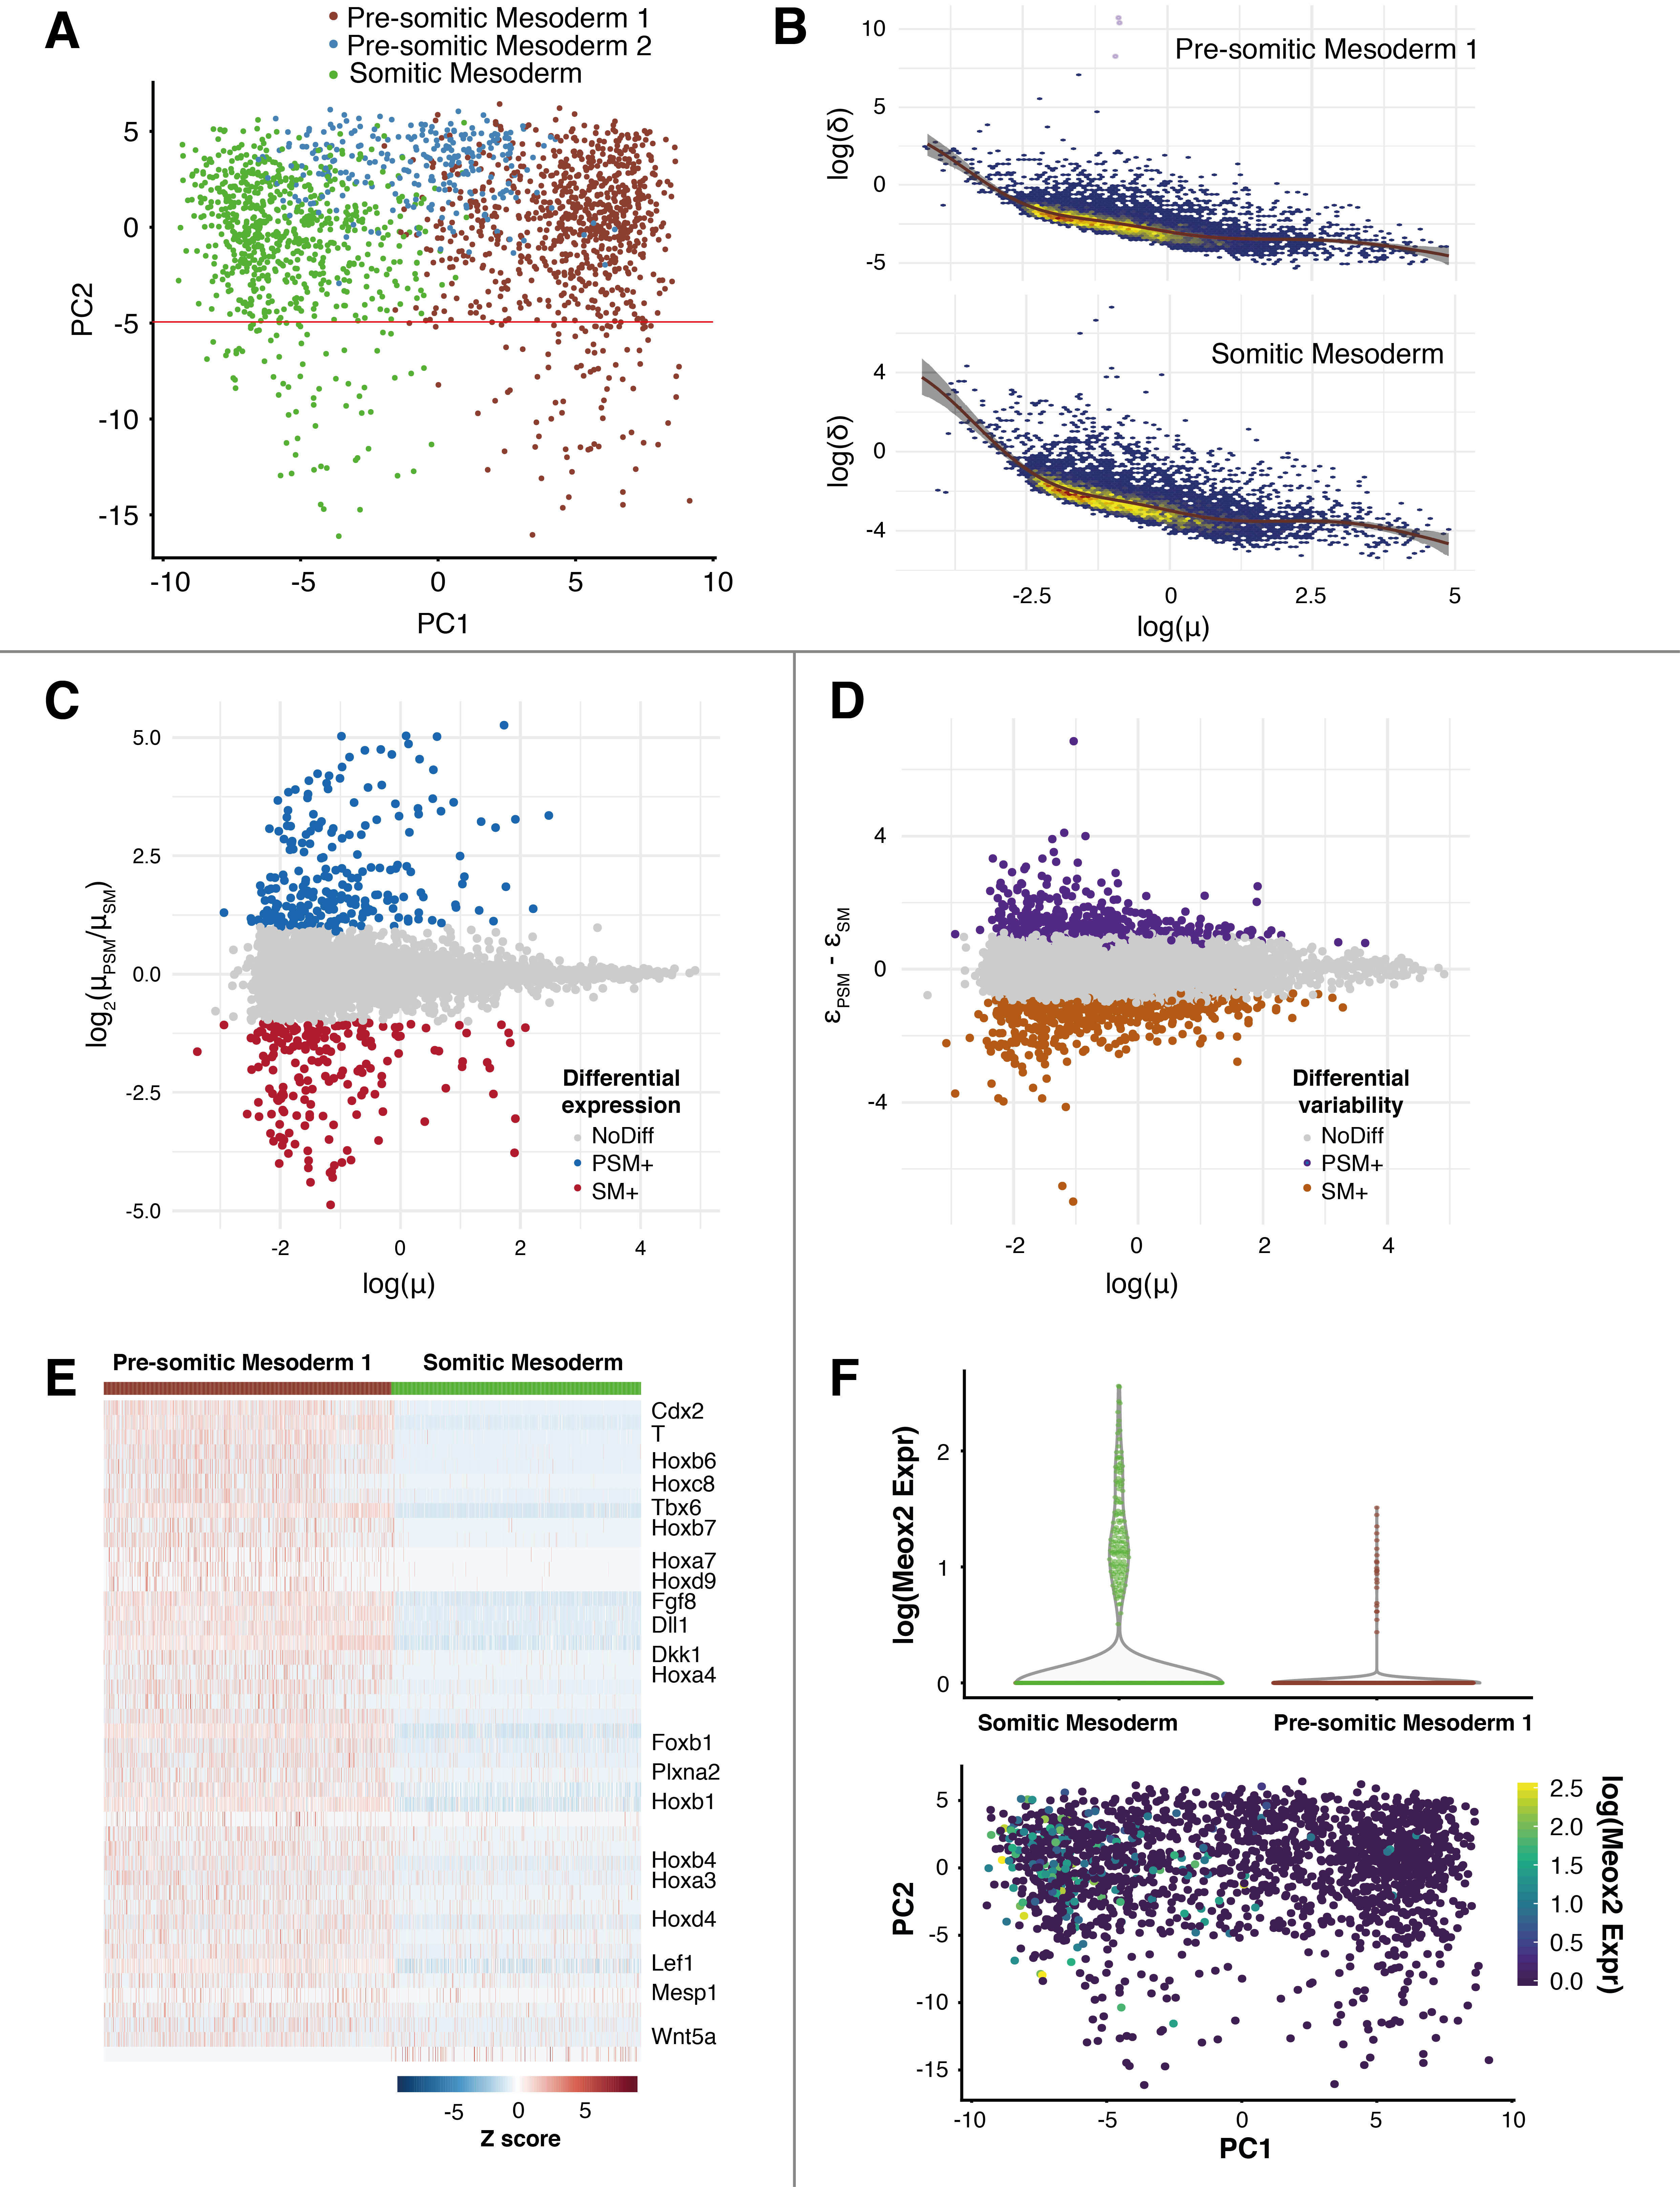
\includegraphics[width=0.8\textwidth]{Fig_14.png}
\caption[Quantification of expression dynamics form droplet-based scRNA-Seq data]{\textbf{Quantification of expression dynamics form droplet-based scRNA-Seq data (Full legend on next page).}}
\label{fig3:variability_schematic}
\end{figure}

\newpage

\captionsetup[figure]{list=no}
\addtocounter{figure}{-1}   
\captionof{figure}{\textbf{Quantification of expression dynamics form droplet-based scRNA-Seq data (continued).}\\
\textbf{(A)} Somitic (SM) and pre-somitic mesoderm (PSM) cells from droplet-based scRNA-Seq data \citep{Ibarra-Soria2018} were selected and visualized in form of a PCA. Colour labelling was done based on the cluster annotation taken from the original publication. For down-stream analysis cells with $\text{PC2}{}<{}-5$ and marked as 'presomiticmesoderm.b'/Pre-somitic mesoderm 2 were removed, \textbf{(B)} For each condition, over-dispersion estimates $\delta_i$ were plotted against mean expression estimates $\mu_i$. The regression trend is indicated as red line, \textbf{(C)} Posterior estimates for the log$_2$ fold change in mean expression between PSM and SM were plotted against mean expression averaged across the two populations. Differentially expressed genes are coloured based on their regulation: blue: PSM-specific (PSM+), red: SM-specific (SM+), \textbf{(D)} Posterior estimates for difference in residual over-dispersion between PSM and SM were plotted against mean expression averaged across the two populations. Differentially variable genes are coloured based on their regulation: purple: PSM-specific (PSM+), brown: SM-specific (SM+), \textbf{(E)} Heatmap showing the Z factor scaled gene expression of pre-somitic mesoderm specific genes of the GO category GO:0009952: anterior/posterior pattern specification. Genes were ordered based on their log$_2$ fold change in expression from highest to lowest, \textbf{(F)} Gene expression of \textit{Meox2} in PSM and SM. This gene was detected to be heterogeneously up-regulated in SM. Upper panel: violin plots showing distribution of log-normalized expression counts. Lower panel: \textit{Meox2} expression across the PCA from \textbf{(A)}.\\}
\captionsetup[figure]{list=yes}

\subsection{Finding continuous changes in variability by linear model fitting}

To detect single genes that continuously increase of decrease in variability, I fit a linear regression to each iteration of the MCMCs sampling $\epsilon_i$ or $\mu_i$ \emph{versus} the group labels \textbf{(Fig.~\ref{fig3:variability_schematic}B)}. The posterior distributions of the slope coefficient were used to categorise genes based on their transcription dynamics along the differentiation time-course (middle panel in \textbf{Fig.~\ref{fig3:linear_variability}}). These categories include: 

\begin{itemize}
\itemsep0em 
\item Increase in mean expression, no change in variability
\item Increase in mean expression, increase in variability
\item Increase in mean expression, decrease in variability
\item Decrease in mean expression, no change in variability
\item Decrease in mean expression, increase in variability
\item Decrease in mean expression, decrease in variability
\item No change in mean expression, no change in variability
\item No change in mean expression, increase in variability
\item No change in mean expression, decrease in variability
\end{itemize}

\newpage

\begin{figure}[!h]
\centering
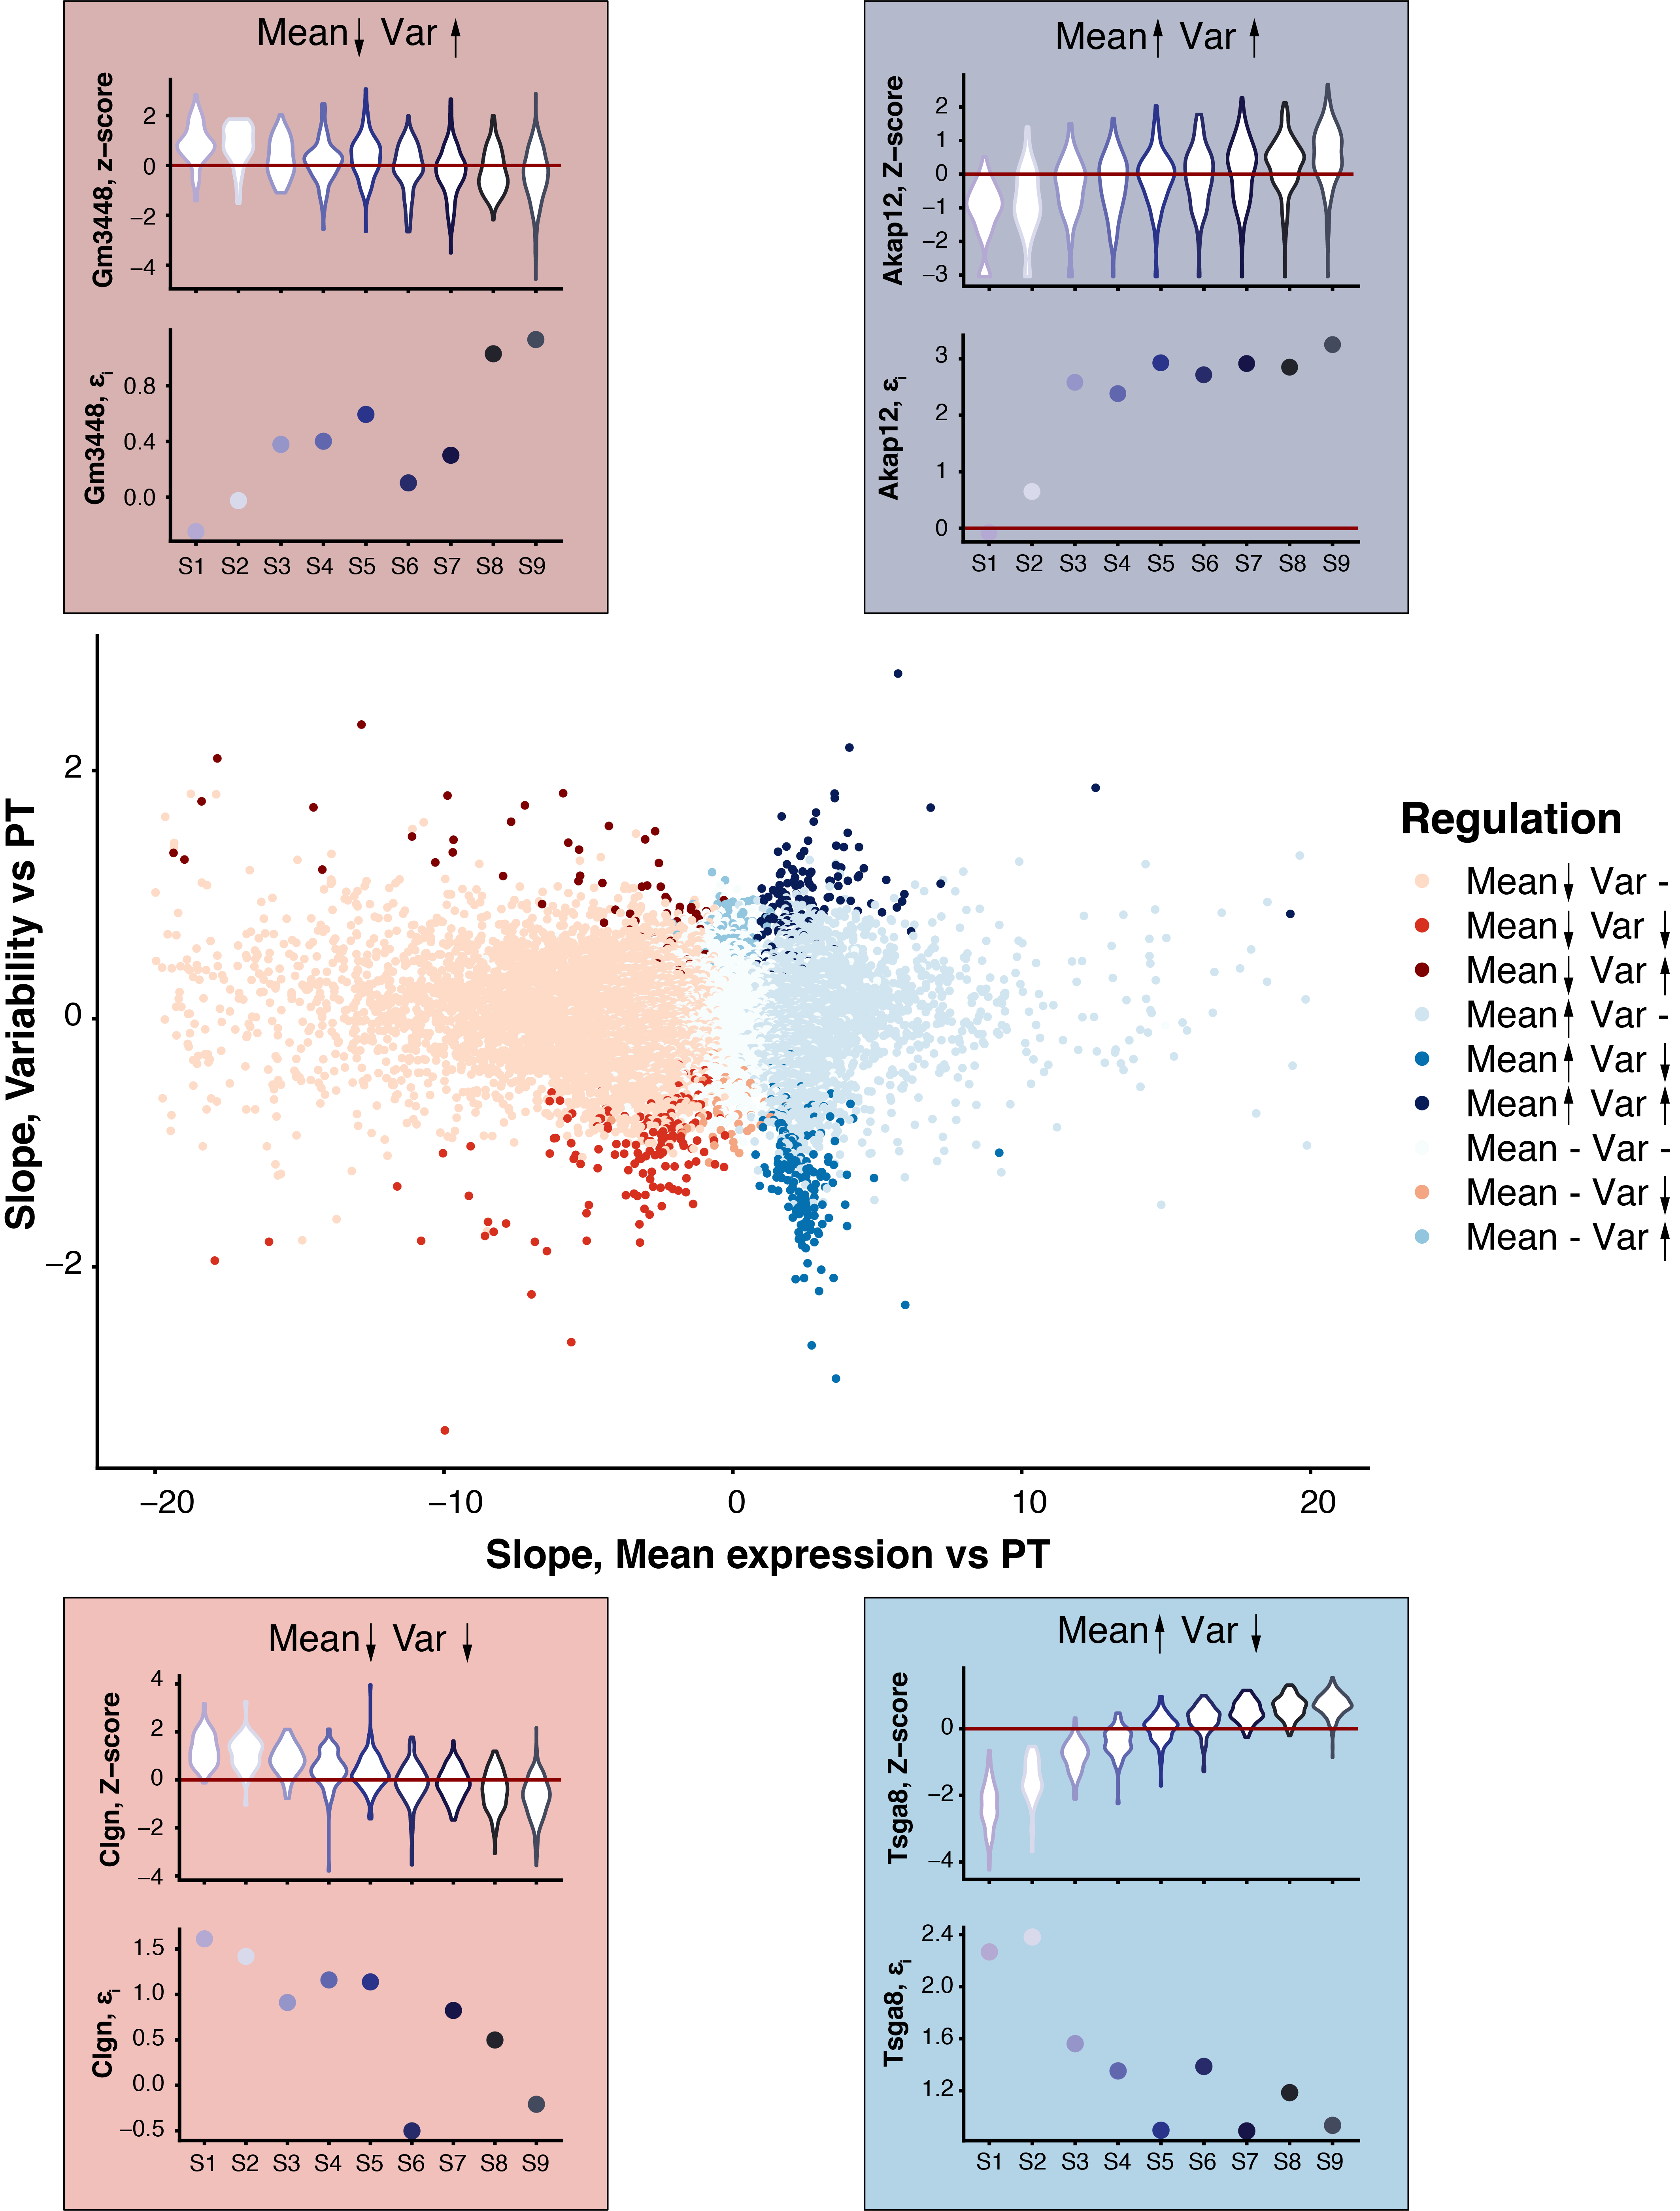
\includegraphics[width=0.8\textwidth]{Fig_15.png}
\caption[Quantification of expression dynamics form droplet-based scRNA-Seq data]{\textbf{Quantification of expression dynamics form droplet-based scRNA-Seq data (Full legend on next page).}}
\label{fig3:linear_variability}
\end{figure}

\newpage

This approach leads to the detection of only few genes that significantly change in variability over the differentiation time-course while the majority of genes change only in mean expression. This can be interpreted as a tight regulation of transcriptional steps during spermiogenesis sperm maturation progresses. Such a process contrasts other differentiation programmes such as hematopoiesis where branching events occur and the whole cell population expands in transcriptional variability to find new attractor states \citep{Mojtahedi2016}. To visualize changes in transcriptional variability, I selected representative genes from four categories: (i) Increase in mean expression, increase in variability, (ii) Increase in mean expression, decrease in variability (iii) Decrease in mean expression, increase in variability, (iv) Decrease in mean expression, decrease in variability (see inlets in \textbf{Fig.~\ref{fig3:linear_variability}}). Interestingly, \textit{Tsga8}, one of the most rapidly evolving X-linked genes, shows a strong increase in expression and a clear decrease in transcriptional variability. \emph{Tsga8} has been reported to be involved in hybrid sterility where F$_1$ crosses of mice form different strains are unable to reproduce. This effect might be due to the strong divergence of the \emph{Tsga8} sequence between species \citep{Good2011}. A tight regulation of its expression during spermiogenesis can therefore further control the phenotypic effect in F$_1$ animals.

\subsection{Clustering of variability profiles}


\newpage

\begin{figure}[!h]
\centering
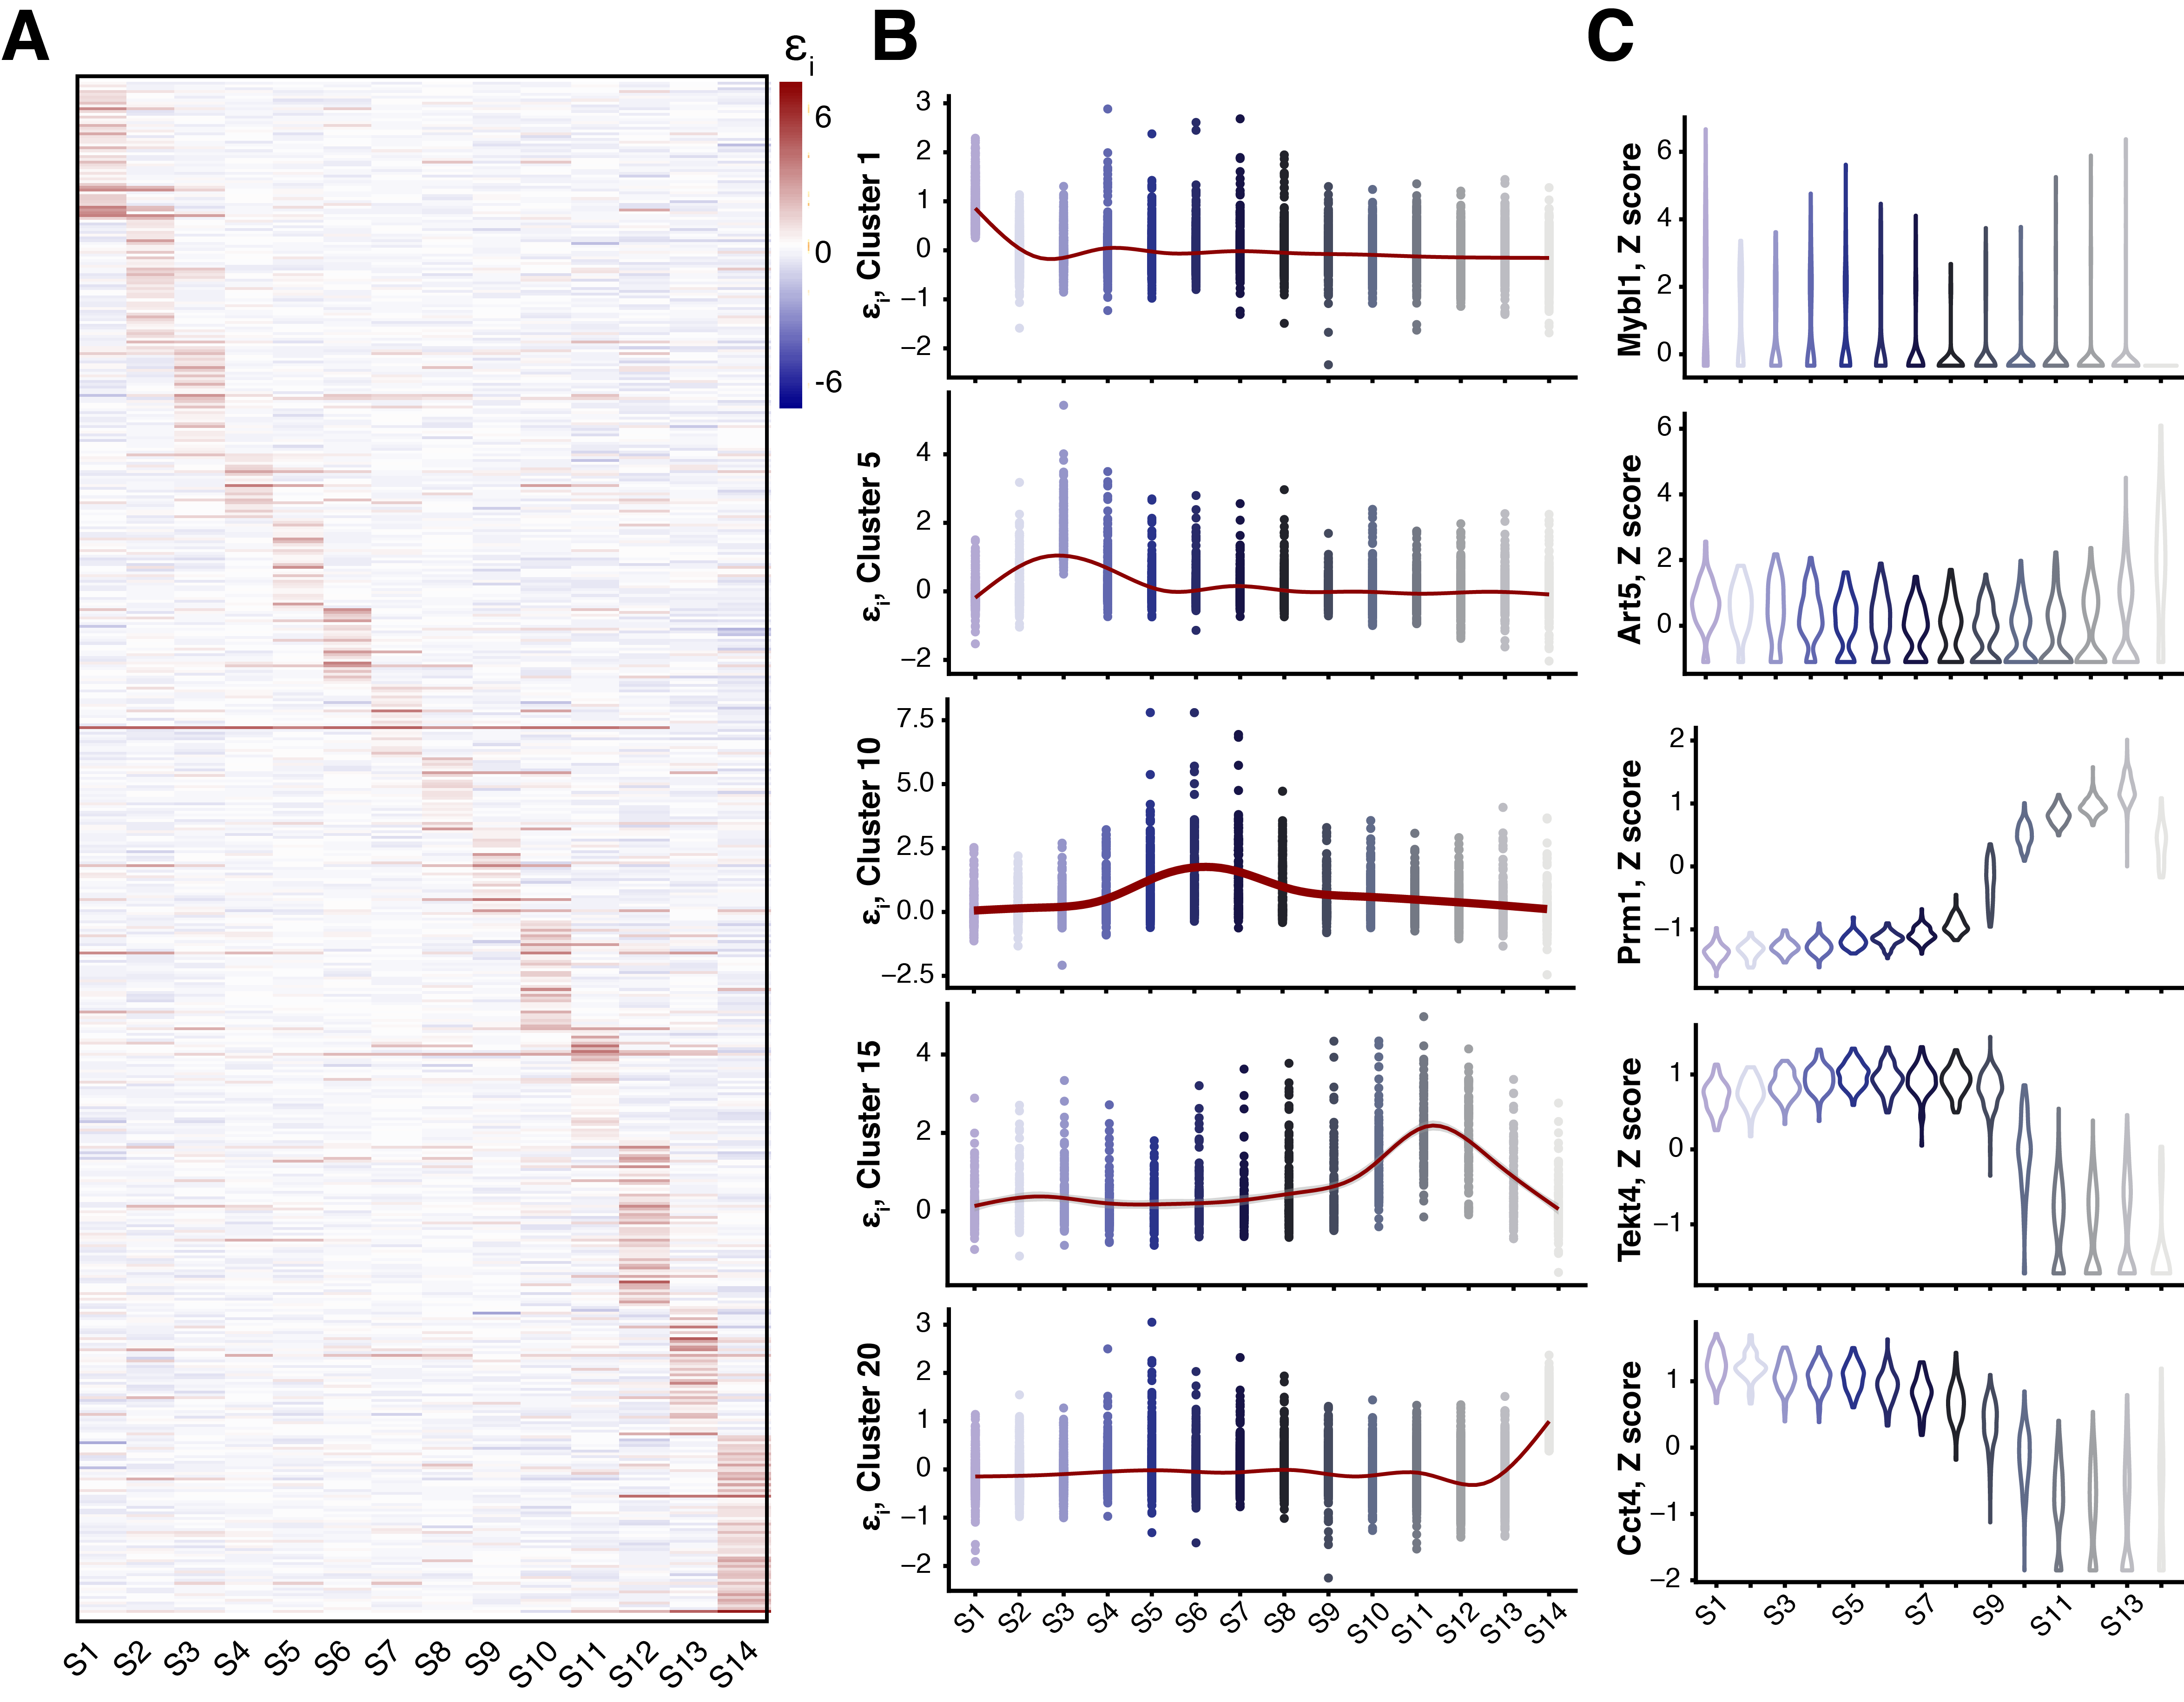
\includegraphics[width=\textwidth]{Fig_16.png}
\caption[Quantification of expression dynamics form droplet-based scRNA-Seq data]{\textbf{Quantification of expression dynamics form droplet-based scRNA-Seq data (Full legend on next page).}}
\label{fig3:linear_variability}
\end{figure}

\newpage



\section{Discussion}

The testes are among the most proliferative tissues in the adult body and ensure fertility via the continuous production of millions of sperm per day. In contrast to most developmental differentiation processes which require the profiling of cellular populations at several time points \citep{Kernfeld2018, Scialdone2016, Wagner2018}, spermatogenesis occurs in continuous waves throughout the reproductive life span, with all intermediate cell types that arise across the ~35 day differentiation program present in adult testes. This provided a powerful opportunity to capture and profile an entire differentiation process by profiling the transcriptomes of thousands of single-cells at a single time point. \\

We identified key developmental transitions within the differentiation trajectory by profiling the first wave of spermatogenesis. Because germ cells have only progressed to a defined developmental point, the differentiation trajectory was truncated, facilitating identification of the most mature cell type. Profiling spermatogenesis in juvenile animals also naturally enriched for rare cell-types that are under-represented in adults. Among these, spermatogonia are of particular interest as these cells not only sustain male fertility, but are also the origin of the vast majority of testicular neoplasms \citep{Bosl1997}. We obtained more than 1100 transcriptional profiles for spermatogonia, allowing the identification of specific cell clusters within this heterogeneous cell population thus greatly improving the resolution over previous studies that only studied adult testes \citep{Lukassen2018}. Furthermore, our approach also enriched for and facilitated characterisation of the complexity within testicular somatic cell types, thus providing a valuable resource for understanding tissue homeostasis.\\

Droplet-based scRNA-Seq can profile large number of cells simultaneously \citep{Klein2015, Macosko2015, Zheng2017}, but often captures cells with a wide range of transcriptional complexity. Consequently, droplet-based assays present a major computational challenge in distinguishing between (i) droplets contain transcriptionally inactive cells versus (ii) empty droplets that contain (background) ambient RNA. By using a stringent default threshold, we identified the majority of somatic and germ cell types in testes, similar to recent single-cell expression studies in mouse and human \citep{Lukassen2018, Xia2018}. In addition, we applied a new statistical method to identify cells from droplet-based data by comparing the ambient RNA profiles \citep{Lun2018}, and were able to identify transcriptionally inactive leptotene/zygotene spermatocytes. This allowed us to bridge the developmental transition between spermatogonia and spermatocytes, thus providing a more complete view of the continuum of germ cell differentiation.\\

Perturbations of the gene expression programme during spermatogenesis frequently result in male sterility by causing a maturation arrest \citep{Cooke2002}. It is therefore of great interest to identify genes with novel spermatogenesis-related functions. To this end, we further characterized the dynamic gene expression patterns underlying meiosis and spermiogenesis. Although transcription broadly increases during meiotic prophase, we detected a diverse set of regulatory behaviours, particularly among spermatocyte-specific genes. In the late stages of spermiogenesis, transcription ceases due to the histone-to-protamine transition. Remarkably, the transcripts from a large set of genes remain highly abundant even after transcriptional shut-down in elongating spermatids. Many of these genes are known to be essential for reproductive success and therefore our analysis likely reveals novel genes with roles in sperm maturation.\\

The transcriptional silencing of the sex chromosomes during meiosis and their subsequent partial re-activation post-meiosis is essential for male fertility \citep{Mahadevaiah2008}. Failure of meiotic sex chromosome inactivation (MSCI) results in the expression of spermatocyte-lethal genes, as demonstrated for two Y chromosome encoded genes zinc finger protein Y-linked (\textit{Zfy}) 1 and 2 \citep{Royo2010}. Our discovery that H3K9me3 is enriched during meiosis at spermatid-specific genes suggests a stronger, targeted repression in spermatocytes for a key subset of X-linked genes. The deposition of H3K9me3 is specific to MSCI in males, and is not observed during general meiotic silencing of unpaired chromosomes (MSUC) \citep{Cloutier2016, Taketo2013, Turner2004a}. Interestingly, when comparing the levels of meiotic silencing for the X chromosome in spermatocytes with the unpaired X chromosome in XO oocytes, the transcriptional silencing was stronger in males compared to females \citep{Cloutier2016}. The deposition of H3K9me3 is linked to more robust silencing of X-chromosomal genes; our finding that spermatid-specific genes are particularly enriched for H3K9me3 in spermatocytes suggests that their repression may be necessary for male fertility. \\

Such a requirement could arise from the opposing evolutionary forces acting on the X chromosome \citep{Rice1992}. Due to its hemizygosity in males, the X chromosome has been predicted to be enriched for male-specific genes. In contrast, meiotic silencing allows pachytene-lethal genes to survive on the X chromosome, since their deleterious effect will be masked by MSCI, similarly to \textit{Zfy1/2} on the Y chromosome \citep{Royo2010}. Our study thus raises interesting questions about how H3K9me3 is targeted to specific genes on the X chromosome in spermatocytes, and how transcription is reactivated in post-meiotic spermatids.


